% honours thesis, main .tex file
% initial comments are from Rose Ahlefeldt

\documentclass[onecolumn,12pt,a4paper,openany,oneside]{book}
\usepackage{anuthesis} % Style file for thesis formatting
\usepackage{fullpage}
\usepackage{layouts}
% Global formatting packages 
\usepackage[T1]{fontenc} % For fonts. Fixes some pdf bugs
\usepackage{lmodern} % fixes some font scaling problem
\usepackage[nottoc]{tocbibind} %Add bibliography/index/contents to Table of Contents
\usepackage{appendix} % To label appendix chapters as "Appendix A, B, C..." instead of "Chapters 7, 8 ,9"
\usepackage{fancyhdr} % To allow more control of headers/footers
\usepackage{hyperref} % hyperlinks for \ref and \cite commands, super useful.
% Maths packages
\usepackage{amsmath,amssymb, amsfonts} % General maths
% Some optional packages
\usepackage{mathtools} % Builds on amsmath, more formatting options
\usepackage{siunitx} %Offers consistent formatting of in-text numbers and units
\usepackage{physics} % bunch of handy physics things, like bra-ket notation

% Tables
\usepackage{booktabs} % Nice table formatting
\usepackage[table,xcdraw]{xcolor}

% Figures
\usepackage{graphicx} % Required for figures
\graphicspath{{./figs/}}

% Bibliography
\usepackage[numbers]{natbib} %Offers more sophisticated bibliographic options
% \bibliographystyle{unsrtnat} % bibliography in order of appearance

% Markup
%\usepackage{showkeys} %Turn this on to list citation keys, reference keys in text
\usepackage[mathlines,pagewise]{lineno} % line numbers

% \usepackage[usenames,dvipsnames]{xcolor}
\newcommand{\jam}{\textcolor{magenta}}

\usepackage{comment}

% If you never plan to print and bind your thesis as a book, you can make the margins even (setlength commands below) you will also need to add the option "openany" to your documentclass
%\setlength\oddsidemargin{\dimexpr(\paperwidth-\textwidth)/2 - 1in\relax}
%\setlength\evensidemargin{\oddsidemargin}

\setlength{\parindent}{0pt}
% Here are the parameters for the page layout. If you modify the template, do not decrease: the font size, the line spacing (1.5), the margin size.\\
% \printinunitsof{mm}{\pagevalues}
% \verb|\marginparwidth|: \printinunitsof{mm}\prntlen{\marginparwidth}
% \pagediagram



%%%%%%%%%%%%%%%%%%%%%%%%%%%%%%%%%%%%%%%%%%
\begin{document}

\pagenumbering{roman} 

\begin{titlepage}
\title{ \textbf{Advanced quantum-mechanical techniques for future gravitational-wave detectors}\\[2cm]}
% title is too similar to: https://link.springer.com/article/10.1007/s41114-019-0018-y ?
\author{\textbf{James W. Gardner}\\[6cm]
\textbf{A thesis submitted for the degree of}\\
\textbf{Bachelor of Philosophy (Honours) with Honours in Physics at} \\
\textbf{The Australian National University}\\[1cm]}
\date{\textbf{\thismonth}}
\maketitle
\end{titlepage}
 
\sloppy


\chapter*{Declaration}
\addcontentsline{toc}{chapter}{Declaration}

This thesis is an account of research undertaken between February 2021 and October 2021 at the Centre for Gravitational Astrophysics, Research School of Physics and Research School of Astronomy and Astrophysics, The Australian National University, Canberra, Australia.

Except where acknowledged in the customary manner, the material presented in this thesis is, to the best of my knowledge, original and has not been submitted in whole or part for a degree at any other university.

The research presented in this thesis was completed on the lands of the Ngunnawal and Ngambri people, the traditional owners of the land of The Australian National University's Canberra campus. I acknowledge that this land was stolen and sovereignty was never ceded, and pay my respects to the elders past and present.

\vspace{20mm}
\hspace{80mm}\rule{40mm}{.15mm}\par
\hspace{80mm} James W. Gardner\par
\hspace{80mm} \thismonth


% include statements effectively insert the contents of the named file. they always start a new page.
\newpage % to fix numbering in ToC
\addcontentsline{toc}{chapter}{Acknowledgements} 
\chapter*{Acknowledgements}
\chaptermark{Acknowledgements}

% supervisors

% squeezer research group for general discussion and support


% collaboration: Xiang Li and Carl Bender


% editorial: dad


% component library for pictures


% friends and family


 

\addcontentsline{toc}{chapter}{Abstract} 
\chapter*{Abstract}
\chaptermark{Abstract}
% self-contained and less than 1 pg!
% no references

% GW, motivation
Gravitational waves are ``ripples'' in spacetime created by massive astrophysical events that carry information about their sources. Within the last decade, interferometric detectors like the Advanced~Laser~Interferometric~Gravitational-Wave~Observatory have used detections of gravitational waves with frequency around 100~Hz from the late inspiral of binary mergers of black holes and neutron stars to learn about such systems.
Gravitational waves around 1~kHz are yet to be detected but could contain other valuable information, e.g.\ 1--4~kHz gravitational waves from the post-merger remnant of binary neutron star systems could be used to further constrain the neutron star equation-of-state and better understand the exotic states of matter within.
% However, gravitational waves are predicted to be emitted from other sources but are yet to be detected because they are outside the sensitive frequency range, and therefore there is valuable astrophysical information that is currently going uncollected. For example, 1--4~kHz gravitational waves from the merger and post-merger remnant of binary neutron star systems are predicted to contain information that could be used to further constrain the neutron star equation-of-state and better understand the exotic states of matter within.
% The ability to detect kilohertz (around 1~kHz) gravitational waves could also lead to better understanding of the origin of low-mass black holes, the post-bounce dynamics of core-collapse supernovae, and the discovery of exotic or primordial sources in the stochastic gravitational-wave background.
% why they can't be seen
% existing proposals for kHz sensitivity
Current interferometric gravitational-wave detectors are not sensitive at kilohertz because of a classical limit on their quantum noise--limited sensitivity and their use of optical cavities, where the quantum noise in the measurement comes from the fundamental quantum uncertainty in the state of the laser light. Existing proposals to improve kilohertz sensitivity use quantum squeezing inside the detector to improve the quantum noise, e.g.\ degenerate internal squeezing, or counter the cavity resonance to improve the response to the gravitational-wave signal, e.g.\ stable optomechanical filtering. However, these two proposals require low optical and mechanical loss, respectively.

In this thesis, I investigate nondegenerate internal squeezing that combines these two existing proposals and has not been fully examined before.
% conclusions
I use an analytic, Hamiltonian model to characterise this configuration's quantum noise--limited sensitivity, stability, squeezing threshold, tolerance to optical loss, and different readout schemes. For a realistic future gravitational-wave detector, I find that nondegenerate internal squeezing is more loss-resistant than degenerate internal squeezing and is a viable, all-optical alternative to stable optomechanical filtering. I also find that it could feasibly improve kilohertz gravitational-wave detection and that using a different readout scheme makes it instead promising for broadband 100--4000~Hz detection. 




\tableofcontents

%\cleardoublepage % Make sure next section starts on a right hand page if using uneven margins

%\linenumbers % This will add linenumbers, which are useful for people proofreading.

% how to remove the "chapter 1" headings on the first page of a chapter: In your chapter itself, instead of "\chapter{First Chapter} use:  \chapter*{First Chapter} \chaptermark{First Chapter} 
% then here, uncomment the below line (which must be before your include statement)
%\addcontentsline{toc}{chapter}{First chapter} 

%%%%%%%%%%%%%%%%%%%%%%%%%%%%%%%%%%%%%%%%%%
% (background chapters)

\chapter{Introduction} %Background: gravitational waves and their detection
\label{chp:introduction}

% introduction: motivation, overview of problem, and what thesis contributes
% written to a general physics audience
% can merge with backgroup chapter/s if appropriate (background chapters are to detail the problem sufficiently and specifically)

%%%%%%%%%%%%%%%%%%%%%%%%%%%%%%%%%%%%%%%%%%
% chapter introduction

% ... (write this later)

	% The detection of gravitational waves from the late inspiral of binary black-hole~\cite{GW150914} and neutron-star~\cite{GW170817} mergers is a landmark achievement of 21st-century physics and engineering that opened up a new field of astronomy dedicated to using gravitational waves to better understand the universe. % might be better in the Abstract?

In this chapter, I motivate the detection of kilohertz gravitational waves, describe what currently prevents us from detecting them, and outline what this thesis contributes to detecting them in the future.

\section{Gravitational waves}
\label{sec:gravWaves}

Gravitational waves are propagating perturbations in spacetime~\cite{}. These perturbations change the proper distance and time between events in spacetime, e.g.\ the proper separation between two massive objects. Since they can move massive objects around, therefore gravitational waves carry energy~\cite{}. %\jam{(``Move'' is problematic, look at choice of frame)}
% Just as they are able to move objects, 
Gravitational waves are emitted by the acceleration of massive objects under certain asymmetry conditions~\cite{}, and since they carry energy the objects that emit them must lose energy by doing so. 
% tense?
Gravitational waves have been detected from the late inspiral of compact binary systems~\cite{} -- meaning that two massive, compact objects, such as two black holes~\cite{}, two neutron stars~\cite{}, or a black hole and a neutron star~\cite{}, were closely orbiting each other. Then, as the binary system lost energy by emitting gravitational waves, the objects got closer together, the orbital frequency increased, and correspondingly the frequency of the emitted gravitational waves increased. Eventually, the objects collided and merged, leaving behind some other object, possibly a black hole or neutron star~\cite{}. The late inspiral of such systems refers to the last moments before the objects collide and merge and therefore to the highest frequency gravitational waves emitted pre-coalescence -- measured at around $100$~Hz~\cite{}. % check this?
Despite being emitted by some of the most massive objects in the universe, the effects of gravitational waves are extremely small -- by the time they reach Earth, even the loudest gravitational waves will only move two objects separated by a kilometre by less than a thousandth the width of a proton~\cite{}. %wordchoice: loudest
This poses a great challenge to detection.

\begin{figure}
	\centering
	% \includegraphics[width=\textwidth]{}
	\caption{Gravitational wave incident on a ring of test particles, evolution over time.}
	\label{fig:GW_ring_of_test_particles}
\end{figure}

Gravitational waves are described by radiative, transverse-traceless solutions to the Einstein field equations of General Relativity~\cite{}. % will need to mention transverse-traceless, quadrupole moment?
The initial amplitude of these waves is described by the quadrupole moment of the source -- a quantity that depends on its distribution of mass which explains why only the most massive astrophysical sources can be detected. % sources closer to the detector can be less massive
% ...
The effect of these waves is to alternately stretch and squash spacetime along the two axes perpendicular to the direction of propagation. That is, a gravitational wave incident normally on a ring of test particles will, over time, stretch and squash one semi-axis of the ring while conversely squashing and stretching the other semi-axis -- as shown in Fig.~\ref{fig:GW_ring_of_test_particles}. \jam{(Clarify expansion of spacetime not change in proper distances)}
By the time the gravitational wave reaches the ring (or detector), however, its amplitude has fallen by the inverse of the distance from the source~\cite{} which is why astrophysical sources with large quadrupole moments only produce small length changes at Earth. % 8.34 in Karl's notes
The unitless gravitational-wave strain at the detector, $h(t)$, gives the change in length $\Delta L$ of a detector's initial length $L$ as $\Delta L(t) = L \;h(t)$. The goal of gravitational wave detection is to measure $h(t)$ as accurately and precisely as possible as it encodes astrophysical information about the source~\cite{}. Henceforth, $h(t)$ is referred to as the gravitational-wave signal, or just: the signal.


	% The orbital period of binary black-hole or neutron-star systems decays as the system radiates away energy in the form of low-amplitude waves in spacetime; these gravitational waves, correspondingly, increase in frequency over time. Current interferometric detectors are most sensitive to gravitational waves in a low-frequency window around 100~Hz that are emitted in the late inspiral of such mergers~\cite{AdvancedLIGO:2015}.

\subsection{Kilohertz gravitational-wave astrophysics} %i.e. sources

% motivate HF limit
All detections of gravitational waves so far have been around $100$~Hz~\cite{}, but there is believed to be varied and interesting astrophysics encoded in higher frequency, kilohertz gravitational waves yet to be detected~\cite{}.
For example, in the merger and post-merger signals from binary neutron-star mergers, which are kilohertz gravitational waves predicted to be emitted during the coalescence and from the remnant object (possibly another neutron star) of the merger. 
Due to the violent nature of the merger, these signals are predicted to contain information otherwise unavailable about the exotic states of matter within neutron stars~\cite{}. Information that could better constrain the possible equations-of-state and improve our understanding of matter under extreme conditions~\cite{miaoDesignGravitationalWaveDetectors2018,}. %this is a bold claim, need another reference? % due to the violent nature, really?
Other astrophysical applications of kilohertz gravitational-wave detection could include determining the origin of low-mass black holes by detecting the merger and ringdown of binary black hole-neutron star mergers~\cite{}, understanding the post-bounce dynamics of core-collapse supernovae~\cite{}, improving measurements of the Hubble constant independently of electromagnetic observations, and searching the stochastic gravitational-wave background for exotic or primordial sources~\cite{miaoDesignGravitationalWaveDetectors2018}.
This possible wealth of new astrophysics motivates developing the ability to detect kilohertz gravitational waves.

% Non-astrophysical sources of gravitational waves?

	% However, the frequency of the emitted gravitational waves then increases beyond this window and so the merger can no longer be observed. In particular, predicted high-frequency gravitational waves around 1--4~kHz from the merger and post-merger remnant of binary neutron-star mergers are yet to be detected. These signals are predicted to contain valuable information that could be used to better constrain the possible equations-of-state of the exotic states of matter within neutron stars~\cite{miaoDesignGravitationalWaveDetectors2018}.
	% Potential astrophysical applications of high-frequency (kilohertz) gravitational-wave detection also include determining the origin of low-mass black holes by detecting binary black hole-neutron star mergers, improving measurements of the Hubble constant independently of electromagnetic observations, and searching the stochastic gravitational-wave background for exotic or primordial sources~\cite{miaoDesignGravitationalWaveDetectors2018}. 

\subsubsection{Sensitivity target for enabling new astrophysics}
\label{sec:GW_kilohertz_target}

% this awkward here, should it be mentioned after Sh is explained? or in the science case?
\jam{(is this necessary here?)}
% this will be the goal of my optimisation
To quantise this goal, consider the case example of the post-merger signal from a binary neutron-star merger. The estimated sensitivity required to reliably detect this signal from a typical source~\footnote{Using current understanding which is conditioned on the very equations-of-state that are to be constrained by these measurements.} is $5\times10^{-25} \mathrm{Hz}^{-1/2}$ from 1--4~kHz~\cite{miaoDesignGravitationalWaveDetectors2018}. This value is for the amplitude spectral density of the noise-to-signal ratio of a detector which will be explained in Chapter~\ref{chp:background_theory}. Other kilohertz astrophysical sources are predicted to require similar or greater sensitivity~\cite{}. For now, all that matters is that I have a target sensitivity for determining whether a given detector will be useful to kilohertz gravitational-wave detection.


%%%%%%%%%%%%%%%%%%%%%%%%%%%%%%%%%%%%%%%%%%
\section{Interferometric gravitational-wave detectors}
\label{sec:intro_IFO}

\begin{figure}
	\centering
	% \includegraphics[width=\textwidth]{}
	\caption{Gravitational wave incident on a Michelson interferometric detector. All configurations in this thesis are simplified for modelling. The gravitational wave moves the end test masses back and forth which changes the interference pattern detected.}
	\label{fig:GW_incident_Michelson}
\end{figure}

% explain what a GWD is 
Current gravitational-wave detectors are based on the Michelson interferometer as shown in Fig.~\ref{fig:GW_incident_Michelson}. An optical Michelson interferometer involves a laser beam being split down two perpendicular arms before returning and interfering at the beamsplitter to produce an interference pattern on a photodetector at the output~\cite{}. 
An incident gravitational wave, imagined as coming into the page in Fig.~\ref{fig:GW_incident_Michelson}, stretches and squashes the lengths of the arms oppositely and changes the path difference between them -- albeit by a relative length change of less than $10^{-21}$~\cite{}~\footnote{Corresponding to $\sim10^{-18}$~m which is far smaller than the wavelength of the carrier laser $\lambda_0\sim10^{-6}$~m and therefore it is not a concern that the interferometer is sensitive to changes only modulo the wavelength of the carrier.}. The resulting change in the interference pattern, known as fluctuations in the interferometer's differential mode, is detected by a photodetector. I assume that the interferometer is tuned such that the light from the arms destructively interferes at the output of the beamsplitter and constructively interferes at the input of the beamsplitter (this ``common'' mode then travels back towards the laser source).
A more complete explanation would explain that \jam{(fix wording)} the gravitational wave can be considered to only move the end mirrors, whose motion phase modulates the light in each arm, which appears as amplitude modulation after the beamsplitter and can be detected, e.g.\ by a photodiode, but the simple explanation above will suffice until a formal model is introduced in Chapter~\ref{chp:proposals}.  

	%Interferometric gravitational-wave detectors are based on the Michelson interferometer as shown in the left panel of Fig.~\ref{fig:coupled_cavities}. A gravitational wave perturbs the path difference between the two arms of the interferometer by stretching and squashing spacetime and the resulting change in the interference of the light at the beamsplitter produces a signal on a photodetector. This change in the interference is known as fluctuations in the differential mode of the interferometer.

% (recall: the effect of a gravitational wave on a ring of test particles in Sect.~\ref{sec:gravWaves})
A problem for interferometric detectors is that the perpendicular axes of deformation are determined by the polarisation of the gravitational wave~\cite{} and so, if the wave is not aligned to the arms, then the response will be less than usual or might vanish. Throughout this thesis, I will ignore this subtlety and assume the maximum detector response: from a gravitational wave exactly aligned to the arms, as this problem can be solved by a global network of detectors with different alignments~\cite{}. % -- like we currently have.

% Michelson signal response function
% unrelated but Another problem for interferometers is that they are only sensitive to phase differences between the arms modulo $2\pi$. %unrelated
Another problem for Michelson interferometers is that the phase accumulated by the light can cancel between going from the beamsplitter to the end mirror and returning from the end mirror back to the beamsplitter.
Therefore the signal transfer function of a Michelson interferometer, $T(\Omega)$, where the spectrum of the measurement of some quantity $\hat{X}(t)$ at the photodetector is $\tilde{\hat{X}}(\Omega) = T(\Omega) \tilde{h}(\Omega) + \text{noise terms}$ , will vanish for periods $2\pi/\Omega$ that are a multiple of the round-trip time of the light in the arms $2L/c$ where $L$ is the length of the arm and $c$ is the speed of light~\cite{}. %($\Omega$ is the angular frequency offset from the carrier frequency, explained further in Chapter~\ref{}) 
I will ignore this complication because the corresponding frequencies $f=\Omega/(2\pi)=c/(2L)=38\mathrm{kHz}$ for the arm length $L=4\mathrm{km}$ of LIGO~\cite{} are far above the kilohertz frequencies of interest (e.g.\ 1--4~kHz for a neutron-star post-merger signal).

\subsection{The role of optical cavities}
% why are there optical cavities

\begin{figure}
	\centering
	% \includegraphics[width=\textwidth]{}
	\caption{Dual-recycled Fabry-Perot Michelson interferometer, the various optical cavities are labelled. Abbreviations: ITM: input test mass, ETM: end test mass, PRM: power-recycling mirror, SRM: signal-recycling mirror.}
	\label{fig:DRFPMI}
\end{figure}

To the base Michelson interferometer, optical cavities are introduced to improve the sensitivity of the detector~\cite{}, principally around $100$~Hz. Three types of cavities are introduced: (1) arm cavities, (2) a power-recycling cavity, and (3) a signal-recycling cavity. 
Firstly, arm cavities (shown in Fig.~\ref{fig:DRFPMI}) are introduced via the placement of an input test mass (labelled as ITM in Fig.~\ref{fig:DRFPMI}) mirror after the beamsplitter, for each arm, forming a Fabry-Perot Michelson interferometer~\cite{}. These cavities significantly~\cite{} increase the circulating power in the arms which broadly improves the interferometer's sensitivity -- which will be shown in Chapter~\ref{chp:proposals}. 
Secondly, to further increase the power, a power-recycling cavity is introduced via a power-recycling mirror (labelled as PRM in Fig.~\ref{fig:DRFPMI}) before the beamsplitter, which reflects some of the otherwise wasted power in the common output mode back into the arms. 
Finally, a signal-recycling cavity is introduced via a signal-recycling mirror (labelled as SRM in Fig.~\ref{fig:DRFPMI}) at the output of the beamsplitter, which enhances the signal response by reflecting the output light back into the arms to be exposed to the gravitational wave for longer. Although the role of the signal-recycling cavity is more complicated than this, it changes the overall resonance behaviour of the interferometer and can be tuned to achieve a variety of outcomes from broadband to narrow-band enhancement~\cite{}, it will suffice until a formal model is introduced in Chapter~\ref{chp:proposals}. 
With these cavities the detector is called a Dual-Recycled Fabry-Perot Michelson interferometer, henceforth referred to as an interferometer. Without the improved circulating power and signal enhancement of these cavities, the detection of gravitational waves at around $100$~Hz would not have been possible~\cite{}, and therefore their inclusion is not optional~\cite{}. 

However, the resonance behaviour of these cavities limits the interferometer's kilohertz signal response. Optical cavities display resonance behaviour due to the different phases acquired by the light at different frequencies on each round-trip of the cavity~\footnote{Note that I will ignore all spatial behaviour of the light throughout this thesis.}. In the steady-state, the light entering a cavity interferes with the light that has undergone one round-trip, two round-trips, and so on. When the cavity is on-resonance for a particular frequency, this interference is constructive and the circulating power in the cavity can increase dramatically beyond the power of the incident light~\cite{}. And when the cavity is off-resonance, the converse is true and the circulating power is low. 
For an interferometer with the arm cavities on resonance at a carrier frequency, for frequency below kilohertz the sensitivity is improved by the power amplification from the arm cavities and the signal response is flat. However, at kilohertz, the arm cavities start going off-resonance and the signal response is far lower (by around an order for Advanced~LIGO~\cite{}) than at $100$~Hz -- although the arm cavities still improve the sensitivity. The other cavities in the interferometer also display resonance behaviour, but the arm cavities are the longest and therefore move off-resonance at the lowest frequency (they have the shortest bandwidth).
%longer arm cavities have shorter bandwidth and therefore matter at lower frequencies, such as kilohertz, as opposed to $10$~kHz etc.. 
Due to the phase interference being modulo $2\pi$, the arm cavity resonance is periodic with frequency $\frac{\omega_\text{FSR}}{2\pi}=\frac{c}{2L_\text{arm}}$, known as one free spectral range (FSR) of the cavity (approximately $37.5$~kHz for 4~km arms), meaning that the cavities will eventually become resonant again. However, I will make a single-mode approximation to the arms that will only be valid for frequencies below the first free spectral range, and so I only discuss the interferometer's response near the first resonance -- which covers the 1--4~kHz range of interest.

	% Arm cavities (circled in green in Fig.~\ref{fig:coupled_cavities}) and a power-recycling cavity are introduced to increase the power within the arms since this increases the sensitivity of an interferometric detector~\cite{1995AuJPh..48..953M}. A signal-recycling cavity (circled in blue in Fig.~\ref{fig:coupled_cavities}) is introduced to further enhance the signal by changing the overall resonance behaviour of the interferometer to increase the time that the light spends coupled to the gravitational wave. Optical cavities display resonance behaviour due to the interference condition on the phase acquired by the light on each round-trip of the cavity. These cavities increase low-frequency sensitivity around 100~Hz and without them, detection would not be possible. However, their resonance behaviour significantly decreases the finite bandwidth of the interferometer and therefore reduces high-frequency (1--4~kHz) sensitivity~\footnote{Only the first resonance of the cavities is considered here because the second resonance is far above (around 37~kHz) the frequency band of astrophysical interest (here, around 1--4~kHz). Moreover, the signal response of the Michelson interferometer falls off at higher frequencies which makes the detector less sensitive at each successive resonance.}. This project considers interferometer configurations that modify the signal-recycling cavity to improve high-frequency sensitivity.

\subsubsection{Simplification to pair of coupled cavities}
% does this need to be in the introduction or can it wait until Chapter 3?
% single mode approximation
\label{sec:coupled_cavity_approximation}

\begin{figure}
	\centering
	% \includegraphics[width=\textwidth]{}
	\caption{Coupled cavity approximation to the interferometer in Fig.~\ref{fig:DRFPMI}. The approximation is only valid when it is below one free spectral range of the arms.}
	\label{fig:coupled_cavity_approx}
\end{figure}


To conceptually simplify the interferometer to make it easier to understand and model, I make a single-mode approximation to the light: (1) in the differential mode of the arm cavities and (2) in the signal-recycling cavity. %Meaning what? Only the light at the carrier frequency is studied? Rather, only the light at one of the sidebands of the carrier frequency?
The motivation for this simplification is that the actual mode in each of the arms is less important than the differential mode of the interferometer which can be approximated as coming from a single ``arm'' cavity~\cite{}, coupled to the signal-recycling cavity, as shown in Fig.~\ref{fig:coupled_cavity_approx}. This is not the same as removing an arm from a Michelson interferometer, the new arm cavity mode is the differential mode of the original interferometer. 
This simplification is common in the literature~\cite{korobkoQuantumExpanderGravitationalwave2019,adyaQuantumEnhancedKHz2020} and, although a more complete understanding requires more modes, is accurate below one free spectral range of the arm cavities~\cite{miaoEnhancingBandwidthGravitationalWave2015,}. In this approximation to the interferometer, the laser source and the power-recycling cavity are abstracted away into the circulating power in the arm cavity which is fixed as an input to the model.
% This simplification allows the interferometer to be understood as a pair of coupled cavities, a two-mode system, and makes clear why certain quantities, like the sloshing frequency of the two modes, should matter to the interferometer -- which is less clear when the interferometer is directly modelled.


\subsection{Factors limiting kilohertz sensitivity}
\label{sec:intro_factors_limiting_kHz}
% explain why current GWD are not sensitive at kilohertz
% what currently prevents us detecting them

Gravitational-wave detectors are not sensitive at kilohertz because: (1) the signal response drops off due to the arm cavity resonance, (2) the noise response is dominated by quantum shot noise that is flat in frequency, (3) the integrated sensitivity (the ratio of the signal response to the noise response) cannot improve by classical means without increasing the circulating power, and (4) the circulating power cannot increase without further technological progress.
The first factor limiting kilohertz sensitivity, the resonance response of the arm cavities, has been addressed above; I address the latter three factors in turn below.

\subsubsection{Noise at kilohertz is shot noise--dominated}
% at kilohertz, going by Buikema et al, 2020: laser intensity and frequency, photodetector dark (electronic) noise, thermal (is falling off)
% It also bears mentioning the other noise sources that affect intereferometers at frequencies below kilohertz: control sensor noise, beam jitter, thermal, seismic, newtonian, gas. But I will not consider any of these in the rest of the thesis.

\begin{figure}
	\centering
	% \includegraphics[width=\textwidth]{}
	\caption{Noise budget of Advanced LIGO from Ref.~\cite{buikemaSensitivityPerformanceAdvanced2020} \jam{(Used without permission? Can I do this?)}. At kilohertz, shot noise dominates and therefore I do not consider other noise sources than quantum noise.}
	\label{fig:Buikemeetal2020_LIGO_noise_budget}
\end{figure}


A real interferometer in subject to noise from many sources, at kilohertz these include, in approximate order of magnitude: quantum shot noise, laser intensity noise, photodetector dark noise, laser frequency noise, and thermal noise~\cite{buikemaSensitivityPerformanceAdvanced2020}~\footnote{Below kilohertz, there are many additional noise sources, such as noise from control systems, beam jitter, seismic noise, Newtonian noise, and gas noise, but I will not consider any of these in this thesis.}. However, at kilohertz, the noise response is dominated by shot noise, with the sum of contributions from all other noise sources making up less than half the total noise~\cite{}, as shown in Fig.~\ref{fig:Buikemeetal2020_LIGO_noise_budget} taken from Ref.~\cite{buikemaSensitivityPerformanceAdvanced2020}. As such, I consider quantum noise as the only noise source throughout this thesis. \jam{(what about thermal noise in sWLC?)}

\begin{figure}
	\centering
	% \includegraphics[width=\textwidth]{}
	\caption{Quantum noise transfer function (top panel), signal transfer function (middle panel), and quantum noise--limited sensitivity shown as noise-to-signal ratio (bottom panel) of a gravitational-wave interferometer. At kilohertz, the sensitivity is limited by shot noise and the decreasing signal due to the arm cavity going off-resonance.}
	\label{fig:simplified_sensitivity}
\end{figure}

To explain briefly, shot noise arises from the fundamental, quantum uncertainty in the phase of a state of light~\cite{} \jam{(check this, the models have noise in every quadrature)}. The vacuum fluctuations of virtual photons at a particular frequency mean that even the vacuum will have some uncertainty, a measurable variance, in its phase, distributed about zero. %phase is not a real thing, mention quadratures
Shot noise is flat in, i.e.\ independent of, frequency which leads it to currently dominate at kilohertz simply because all other noise sources have been reduced below it by decades of research and innovation~\cite{}. For sensitivity, approximated henceforth as quantum noise--limited sensitivity, the ratio of the signal response to the quantum noise response of the interferometer, because the signal is decreasing and the shot noise is constant, the sensitivity decreases at kilohertz, as shown in Fig.~\ref{fig:simplified_sensitivity}. It is conventional to show sensitivity as the noise-to-signal ratio (also known as signal-normalised noise) in the gravitational-wave literature, so lower values indicate better sensitivity in the bottom panel of Fig.~\ref{fig:simplified_sensitivity}.
A detailed explanation of quantum noise will be given in Section~\ref{sec:qnoise}.


\subsubsection{Limit on integrated sensitivity}
%limit on the quantum noise--limited sensitivity
% mizuno limit (due to QCRB) on the integrated sensitivity, i.e. on the bandwidth-peak sensitivity product --> can be beaten by squeezing

The Mizuno limit states that the circulating power within the arms limits an interferometer's integrated sensitivity, i.e.\ the product of its bandwidth and peak sensitivity~\cite{miaoFundamentalQuantumLimit2017}.
This limit comes ultimately from the Quantum Cramer-Rao Bound where the circulating power quantifies the total energy of the detector~\cite{} \jam{(explain the physics?)}.
For a fixed circulating power, this limit means that improving bandwidth to include kilohertz sensitivity would sacrifice peak sensitivity across the band, compromising existing low-frequency ($\sim100$~Hz) sensitivity. % beyond the point of being useful for detection. %justify this?
While this thesis is motivated by kilohertz detection, this low-frequency sensitivity should be maintained. For the case example of observing binary neutron-star mergers, maintaining low-frequency sensitivity would allow for the pre-merger inspiral to be seen, hopefully along with the merger and post-merger remnant at kilohertz, necessary to construct the full description of the merger~\cite{}.
Therefore, this limit poses a problem to improving sensitivity at kilohertz to that required for detection.


\subsubsection{Technological limitation: circulating power}
\label{sec:circulating_power}
% Why can circulating power not increase?
% constraints for future detectors
% I assume that we can't increase power by a factor of 2, unlike Miao et al 2018

The Mizuno limit on improving kilohertz sensitivity could be alleviated if the circulating power could be increased, however, this is not currently technologically possible. In Advanced~LIGO, which operates at $750$~kW circulating power in the arms, point absorbers on the optics~\cite{Brooks_2021} and parametric instabilities (particularly when a large number of unstable modes are available)~\cite{PhysRevLett.114.161102} prevent increasing the circulating power far beyond its current value. This poses a technological challenge to future detectors which demand upwards of $3$~MW for LIGO~Voyager~\cite{} and $4.5$~MW for NEMO~\cite{}, a challenge yet to be solved but with much progress towards it~\cite{}. %\jam{(Need further information? For Evans et al, 2015, didn't they alleviate the parametric instability problem?)}
Therefore, I will assume that $\sim3$~MW circulating power is the maximum achievable value for the next generation of detectors, assuming significant technological progress in the coming decades. Since arbitrary circulating power is not possible, a different method is required to improve kilohertz sensitivity.


	% The amount of laser power within an interferometric gravitational-wave detector limits how much its high-frequency sensitivity can improve without its low-frequency sensitivity worsening or the power needing to increase~\cite{miaoFundamentalQuantumLimit2017}. 
	% However, gravitational waves require a wide band of sensitive frequencies to detect as they are typically not monochromatic~\cite{miaoDesignGravitationalWaveDetectors2018}, and further increasing the power is technologically problematic~\cite{Brooks_2021,PhysRevLett.114.161102}. 

\subsubsection{How to improve kilohertz sensitivity}

\jam{(This is a tiny literature review, move the other here or indicate that I will examine dIS and sWLC much more closely later.)}
The above four factors: the arm cavity resonance, shot noise, the Mizuno limit, and power limitations, can be avoided and kilohertz sensitivity can be improved, but this requires changes to the detector's configuration.
I will review the literature of proposals to improve kilohertz sensitivity in Section~\ref{sec:literature_review}. For now, I will briefly mention two recent proposals: (1) degenerate internal squeezing~\cite{korobkoQuantumExpanderGravitationalwave2019,adyaQuantumEnhancedKHz2020} and (2) stable optomechanical filtering~\cite{liBroadbandSensitivityImprovement2020}. 
The Mizuno limit, due to its origin from the Quantum Cramer-Rao Bound, can be avoided by non-classical techniques, such as squeezing~\cite{}, a technique which trades off the quantum uncertainty in a desired quantity for that in a less desired quantity, detailed in Chapter~\ref{chp:background_theory}. Squeezing is already used in Advanced~LIGO externally to the coupled cavities to halve the shot noise~\cite{tseQuantumEnhancedAdvancedLIGO2019} across the band. Degenerate internal squeezing is a proposal that uses squeezing instead inside the signal-recycling cavity to further enhance the sensitivity by interacting with the signal and noise, which I will detail in Section~\ref{sec:dIS}. 
The Mizuno limit can also be avoided by making the arm cavity more broadly resonant through introducing a filter cavity. This ``white-light cavity'' idea~\cite{miaoEnhancingBandwidthGravitationalWave2015,} is what stable optomechanical filtering achieves by coupling a mechanical mode to the signal-recycling cavity mode, which I will detail in Section~\ref{sec:sWLC}.
% although frontrunners in the literature~\cite{}
However, these two configurations have their problems. Degenerate internal squeezing is susceptible to optical loss because the configuration decreases the signal and relies on correlations degradable by optical losses~\cite{korobkoQuantumExpanderGravitationalwave2019}. Stable optomechanical filtering requires low mechanical loss which demands better thermal noise and mechanical quality factor than are currently technologically possible~\cite{liBroadbandSensitivityImprovement2020,miaoEnhancingBandwidthGravitationalWave2015}. These problems could limit the feasibility of these two configurations for kilohertz detection, and therefore they motivate looking for alternative configurations. %But any alternative proposal must first avoid the limit set by the above four factors.


%%%%%%%%%%%%%%%%%%%%%%%%%%%%%%%%%%%%%%%%%%
\section{Thesis outline}
% what the thesis contributes towards the problem: the aims from the research proposal
% quantum noise--limited sensitivity
% overview of the problem: we can't see at HF, (to be covered) and the problems with exisiting proposed solutions (the latter will be detailed more in the relevant background chapters)

In this thesis, I examine an alternative gravitational-wave detector configuration, nondegenerate internal squeezing, that combines the three-mode structure of stable optomechanical filtering with the all-optical approach of degenerate internal squeezing, with the aim that it might be more feasible for kilohertz gravitational-wave detection. This configuration improves kilohertz sensitivity by using squeezing to get around the Quantum Cramer-Rao Bound. This means that it does not require increased circulating power nor, a priori, compromised low-frequency sensitivity. Although this configuration has been briefly mentioned in the literature as the lossless Hamiltonian is equivalent to stable optomechanical filtering~\cite{liBroadbandSensitivityImprovement2020}, no work has, as yet, studied it in detail nor assessed its feasibility for kilohertz detection~\cite{}. The goal of this thesis is to fill that gap in the literature.

I will first review the background theory of quantum noise and squeezing in Chapter~\ref{chp:background_theory} to be able to describe the quantum noise response of a detector. In this chapter, I will demonstrate the analytic, Hamiltonian model that I will use throughout the thesis on the simple, well-known cases of degenerate and nondegenerate optical parametric oscillators~\cite{}. I will also discuss the current use of squeezing externally to the interferometer. Next, in Chapter~\ref{chp:proposals}, I will review the literature of proposals to improve kilohertz detection and will focus on the two proposals that I will compare my work against, degenerate internal squeezing and stable optomechanical filtering. This chapter will demonstrate the Hamiltonian modelling to calculate the quantum noise--limited sensitivity of degenerate internal squeezing. I will discuss the benefits and problems with these two configurations and motivate combining them into nondegenerate internal squeezing.

% quantum optics of nIS
% GW detection science case for nIS
I will derive an analytic, Hamiltonian model of lossy nondegenerate internal squeezing in Chapter~\ref{chp:nIS_analytics}. This derivation will be based on and justified by the models in the previous two chapters. Using the model, I will characterise the stability and sensitivity of the configuration, demonstrate its reduction to known models in high and low loss limits, and derive the limit of the amount of available squeezing.
Next, in Chapter~\ref{chp:science_case}, I will consider applying nondegenerate internal squeezing to kilohertz 1--4~kHz and broadband 100--4000~Hz gravitational-wave detection. I will consider its tolerance to realistic optical losses and show which optical losses dominate the noise. Using realistic optical loss and the parameters of a future detector, I will then compare nondegenerate internal squeezing to the two existing proposals. I will show that it is more loss-resistant than degenerate internal squeezing, although the sensitivity curves are not directly comparable, and that the amount of optical loss to match the performance of stable optomechanical filtering with low mechanical loss is at least as feasible as that low mechanical loss. I will find that the improvements to kilohertz and broadband sensitivity are promising.
Finally, in Chapter~\ref{chp:idler_readout}, I will consider alternative readout schemes which change which optical field is measured for nondegenerate internal squeezing. I will characterise them similarly to the readout scheme in the previous chapters and discuss the differences between them and the previous readout scheme. I will show that the broadband sensitivity can be improved by combining different readout schemes which is an advantage of the configuration.
I will finish in Chapter~\ref{chp:future_work_and_conclusions} by considering the conclusions and limitations of my work and what avenues of future work it suggests.

% return to the motivation
% The work in this thesis also has broader applications to cavity-based quantum metrology.
This thesis also contributes some work to the broader field of cavity-based quantum metrology. While the motivation behind this work is to detect kilohertz gravitational waves and advance astrophysics through observing new sources, the results in this thesis could be applied to other problems, such as axion detection for dark matter~\cite{}.


\jam{(Include a statement of contributions?)}

\jam{(Include a list of abbreviations? E.g.\ SNR, NSR, LIGO, KAGRA, NEMO, OPO, PT, DC, ITM, ETM, SRM, PRM, SRC. And/or a list of symbols for the analytic models?)}


% From research proposal
	% I aim to design and analytically model an all-optical interferometer configuration to improve high-frequency sensitivity beyond current detectors, while neither fully sacrificing low-frequency sensitivity nor increasing the power. I will include realistic sources of loss in the model to assess the feasibility of this configuration. Finally, I will compare this configuration to existing proposals to show the potential benefits of its design.

	% The central aim of this project is to investigate nondegenerate internal squeezing and assess how it might improve the high-frequency sensitivity of future detectors. Although nondegenerate internal squeezing has been considered before, no work has fully examined it nor assessed its feasibility by including losses in the model~\cite{liBroadbandSensitivityImprovement2020}. I will perform an analytic investigation of nondegenerate internal squeezing that will include a feasibility assessment using losses and realistic assumptions and conclude with a comparison to previously proposed configurations.

	% I will use a Hamiltonian method to analytically model nondegenerate internal squeezing and
	% calculate its quantum-noise limited sensitivity. The Hamiltonian for nondegenerate internal
	% squeezing is already known for the approximate interferometer model of a pair of coupled cavities shown in the right panel of Fig.~\ref{fig:coupled_cavities}~\cite{korobkoQuantumExpanderGravitationalwave2019,liBroadbandSensitivityImprovement2020}. %cite Schori et al?
	% This Hamiltonian includes standard harmonic oscillator terms for each of the optical fields in each cavity and at each frequency and interaction terms that represent the squeezing process and coupling between the cavities. I will solve the quantum Langevin equations of motion to find the output signal and noise fields that are measured by the photodetector and calculate the sensitivity of the overall detector. These equations combine the Heisenberg equations of motion of the field operators with input/output terms. To solve them, I will use common approximations including a semi-classical approximation of the pump field to treat it as a reservoir and a linear expansion in small fluctuations around the expectation values of certain operators. This Hamiltonian method and the approximations involved are widely used in the literature and, in particular, in the works that I will compare to and base my derivation upon~\cite{liBroadbandSensitivityImprovement2020,korobkoQuantumExpanderGravitationalwave2019}. I will repeat the analysis of stable optomechanical filtering done in Ref.~\cite{liBroadbandSensitivityImprovement2020} to practice this Hamiltonian method before attempting the novel derivation of nondegenerate internal squeezing with realistic assumptions.

	% I will assess the feasibility of nondegenerate internal squeezing by studying the effects of various noise sources on the sensitivity under realistic assumptions. The degenerate internal squeezing literature suggests that optical loss will be the dominant noise source of nondegenerate internal squeezing~\cite{korobkoQuantumExpanderGravitationalwave2019}. Therefore, I will prioritise including optical loss in the model above other noise sources. I will also include photodetector loss to test the hypothesis that nondegenerate internal squeezing is more resistant to photodetector loss than degenerate internal squeezing. Under realistic assumptions about improvements in optical loss and squeezing beyond current detectors, I will compare the sensitivity of the model to the estimated sensitivity required to detect a typical binary neutron-star post-merger signal~\cite{miaoDesignGravitationalWaveDetectors2018}. This will determine how large an improvement in these factors will need to be achieved, technologically, before the configuration is physically viable.

	% Finally, I will compare nondegenerate internal squeezing to degenerate internal squeezing and stable optomechanical filtering by comparing the sensitivity and feasibility of the three systems. Nondegenerate and degenerate internal squeezing have not been compared before. Similarly, although the connection has been previously made between the Hamiltonians of nondegenerate internal squeezing and stable optomechanical filtering~\cite{yapadyaPersonalCommunication,liBroadbandSensitivityImprovement2020}, the sensitivity and feasibility of the two systems have not been compared before. The deeper connection to stable optomechanical filtering means that I will prioritise comparing my model to it over degenerate internal squeezing.


%%%%%%%%%%%%%%%%%%%%%%%%%%%%%%%%%%%%%%%%%%
\section{Chapter summary}

% In this chapter, I motivate the detection of kilohertz gravitational waves, describe what currently prevents us detecting them, and outline what this thesis contributes to detecting them in the future.

In this chapter, I have described gravitational waves and motivated the detection of kilohertz gravitational waves for advancing our astrophysical understanding of neutron stars, black holes, and supernovae. I have explained how detectors based on the Michelson interferometer can detect gravitational waves at around $100$~Hz, why cavities are introduced into these detectors, and why these detectors' sensitivity cannot be simply broadened to detect kilohertz gravitational waves. Finally, I have mentioned the two proposed configurations that motivate my work (degenerate internal squeezing and stable optomechanical filtering), what problems these configurations face, and that this thesis will examine nondegenerate internal squeezing as an alternative configuration for gravitational-wave detection.


 
	% motivation: kHz gravitational wave detection could lead to new physics
	% the problem: cannot increase power but want to increase HF sensitivity without sacrificing LF sensitivity
	% aims
	% outline

\chapter{Background theory: quantum noise in interferometric gravitational-wave detectors}

% this chapter has a lot of ideas, need to figure out the logical flow -- look at research proposal and other theses --> talk to supes

% do I need to start as far back as MJ's thesis? i.e. back at the quantisation of light, definition of quadratures etc.?

%%%%%%%%%%%%%%%%%%%%%%%%%%%%%%%%%%%%%%%%%%
\section{Quantum noise}

% HUP

\subsection{Optical loss}
%  source of loss, realistic values (now and in a few decades time, 100 years time etc.)

% \subsubsection{Technological limit: optical loss}


\section{Squeezing}


% \section{Squeezed cavity (OPO) - analytic model}

Although this derivation is widely available in the literature~\cite{}, I include it here to demonstrate the Hamiltonian method that I use throughout the rest of the thesis. \jam{Should this be included in an appendix?}


\subsection{Degenerate OPO}

% OPO = squeezed cavity with no seed light

\subsubsection{Threshold}


\subsection{Nondegenerate OPO}


\subsubsection{Threshold and idler loss}


\subsection{External squeezing in interferometric gravitational-wave detectors}

% Generally speaking, the vacuum entering the main port of an arbitrary quantum noise--limited detector can be squeezed externally and injected via a Faraday isolator (a directional beam-splitter) to lower the quantum noise.

\subsubsection{Technological limit: pump power} 
% i.e. threshold

%%%%%%%%%%%%%%%%%%%%%%%%%%%%%%%%%%%%%%%%%%
\section{Chapter summary}

Beyond better external squeezing, there are many \jam{(are there?)} existing proposals to improve the kilohertz sensitivity of gravitational-wave detectors. In the next two chapters, I examine two of the front-runners: degenerate internal squeezing and stable optomechanical filtering.
\jam{(justify somewhere that these are the front-runners and that there are not other configurations that I should be considering -- literature review!)}


	% Mizuno limit
	% cannot increase power
% Squeezing to improve quantum noise--limited sensitivity
	% mechanism of squeezing
	% optical loss
	% external squeezing
	% remaining problem of how to further increase kHz sensitivity

% should this background chapter be broken up? GWD's separately then theory of quantum noise?

\chapter{Existing proposals for improving kilohertz sensitivity} % Background: existing proposals for improving kilohertz sensitivity
\label{chp:proposals}
%%%%%%%%%%%%%%%%%%%%%%%%%%%%%%%%%%%%%%%%%%
% chapter introduction
% Beyond better external squeezing, there are many \jam{(are there?)} existing proposals to improve the kilohertz sensitivity of gravitational-wave detectors. In the next two chapters, I examine two of the front-runners: degenerate internal squeezing and stable optomechanical filtering.
% demonstrate modelling again, for the third and last time before my model -- much of the maths should be quite familiar by now
% set-up the problem: how do these configs get past the four factors in the introduction and why aren't they good enough for kilohertz sensitivity

In this chapter, I consider some of the existing solutions to solve the problem of increasing kilohertz sensitivity outlined in Section~\ref{sec:intro_factors_limiting_kHz} which motivate the configuration I examine. After first summarising the literature, I focus on two promising proposals: degenerate internal squeezing~\cite{} and stable optomechanical filtering~\cite{}. I use the tools of the previous chapter to understand and model degenerate internal squeezing and demonstrate how I will approach my research. Then, I discuss stable optomechanical filtering using the same ideas. %, although I do not present a separate model of it for reasons that will become clear. 
%Stable optomechanical filtering is the optomechanical analogue of my all-optical configuration which implies that there is . 
While promising, these existing proposals have problems with their tolerance to different losses: optical and mechanical loss, respectively. This motivates my research in the following chapters into a configuration that is closely related to these proposals but might be able to overcome these problems and better improve kilohertz sensitivity.


%%%%%%%%%%%%%%%%%%%%%%%%%%%%%%%%%%%%%%%%%%
\section{Literature review}
\label{sec:literature_review}
% should be categorising and judging

% John Close says: don't just list papers, a powerful review identifies the goal of the thesis and puts it in context, ideally quantitatively --> what are the quantities for my thesis, sensitivity?

\jam{(The role of this section is (1) to explain why I look at these two configurations and (2) satisfy the thesis requirement for a literature review, which I need to look up in the honours material. Do I need more citations or critical analysis, perhaps?)}

% intro: beyond external changes (external squeezing and caves's amplifier) to interferometer and increasing circulating power
Various solutions to improve the kilohertz sensitivity of gravitational-wave detectors has been given in the literature~\cite{}. Any proposal to do so without increasing circulating power or degrading existing sensitivity must overcome the Mizuno Limit through some non-classical technique \jam{(how does sWLC avoid Mizuno limit? why is cancelling arm cavity resonance non-classical?)}, as outlined in Section~\ref{sec:intro_factors_limiting_kHz}. Broadband improvement is possible through external modifications to the interferometer such as external squeezing and Caves's amplification, as already discussed, but I am interested in techniques that directly address kilohertz sensitivity. In this review, I will summarise: (1) the existing gravitational-wave detectors around the world, (2) the future, third-generation detectors under conceptualisation and construction \jam{(are they being constructed right now?)}, (3) the proposals that use internal squeezing, (4) the proposals that use optomechanical filtering, and (5) some of the other existing proposals. %However, I will refrain from a thorough technical explanation of these configurations, which will be given later in this chapter. 

\jam{(I will need to do more reading to write this section convincingly. See supervisors for citations. Do I need to really review detectors?)}
% existing detectors
The global network of existing gravitational-wave detectors consists of Advanced~LIGO~\cite{} (Hanford~\cite{} and Livingston~\cite{} sites), Advanced~Virgo~\cite{}, KAGRA~\cite{}, and GEO600~\cite{} \jam{(check this list)}. All of these follow the interferometer design discussed in Section~\ref{sec:intro_IFO} with the only major change relevant for quantum noise \jam{(check this)} being the use of external squeezing in Advanced~LIGO, discussed in Section~\ref{sec:external_squeezing}. I will use Advanced~LIGO to represent this generation, henceforth. 
% 3rd generation detectors: LIGO Voyager, NEMO, Einstein Telscope, Cosmic Explorer --> why I will focus on the Voyager parameter set (no increased circulating power, no change in arm lengths)
The proposed next, third generation of \jam{(ground-based)} detectors consists of LIGO~Voyager~\cite{}, NEMO~\cite{}, Einstein~Telescope~\cite{}, and Cosmic~Explorer~\cite{} \jam{(check 2.5 versus 3 generation)}. These still use the same interferometer design \jam{(with the exception of NEMO~\cite{}?)} \jam{(check this)} but differ from the previous generation in the interferometer parameters, such as the circulating power, arm length, test mass mass, carrier wavelength, and transmissivities of the input test mass and the signal-recycling mirror~\cite{}. 
The later detectors, Einstein~Telescope and Cosmic~Explorer, are proposed to have significantly longer arm lengths and higher circulating powers than LIGO~Voyager or the current generation of detectors. 
I will consider the feasibility of configurations using the LIGO~Voyager parameter set~\cite{} because it will be the first of these future detectors to come online as it is a series of upgrades to the existing Advanced~LIGO detectors~\cite{}. Moreover, variations of the LIGO~Voyager parameter set are often used in the literature to assess the configurations in this chapter~\cite{Li2020,Miao2018,Korobko,}. In particular, I will use $3$~MW circulating power, $4$~km long arm cavity, $56$~m long signal-recycling cavity, $200$~kg test masses, and $2~\mu\text{m}$ carrier wavelength~\footnote{There is debate about $2$ versus $1.064~\mu\text{m}$ as the preferred carrier wavelength~\cite{}, e.g.\ different photodiode efficiencies~\cite{}. I will not consider this because my models are too simplified to compare the technological constraints.}, but I will vary the transmissivities away from their values of $0.002$ for the input test mass and $0.046$ for the signal-recycling mirror to test the effects of changing the respective coupling rates~\footnote{There is a subtlety here, these parameters might be biased against one configuration over another. I have mitigated this by varying the coupling rates between the modes which appears to well characterise the different classes of parameter sets~\cite{}.}. 

% separate from these defined detectors is a literature of different possible configurations and proposals for these and future detectors.
These future detectors have established science-cases \jam{(colloquial?)} and detailed proposals, but separate from them in the literature is much exploratory work which could be realised in a non-specific future detector, and this is where my work fits into. %~\footnote{It is worth clarifying here that I am not aiming to produce a complete proposal for a future detector either, only explore the space of designs}.
% degenerate internal squeezing
One such proposal is degenerate internal squeezing (also known as a degenerate quantum expander)~\cite{Korobko2019,Adya2020}, which has been considered for NEMO~\cite{}. 
Degenerate internal squeezing was first proposed in Ref.~\cite{Korobko2019} and has been subsequently characterised in Refs.~\cite{Adya2020,Korobko?,}. 
% I will explain this configuration thoroughly later,
This configuration has a squeezer inside the signal-recycling cavity, turning the two-cavity interferometer into an OPO coupled to the arm cavity. Unlike external squeezing, where only the readout port vacuum is squeezed, degenerate internal squeezing also squeezes the intra-cavity noise and the gravitational-wave signal. Although de-amplifying (squeezing) the signal is not ideal, the reduction in the quantum noise is significant enough to produce an improvement in sensitivity. This improvement can occur at kilohertz if the interferometer parameters are chosen correctly~\cite{}. However, degenerate internal squeezing is sensitive to intra-cavity and detection losses, since these losses reduce the signal but amplify the noise towards vacuum. 
Research into degenerate internal squeezing continues today~\cite{}, e.g.\ for its ability to be switched into an anti-squeezing regime in the high loss limit~\footnote{This limit is beyond the expected losses in future detectors, e.g.\ above $50\%$ compared to $10\%$, but it demonstrates that internal anti-squeezing is useful under certain circumstances.}~\cite{KorobkoTalk}, which improves sensitivity similarly to a Caves's amplifier, see Section~\ref{sec:cavess_amp}, except that the amount of anti-squeezing can be different for signal and noise.
% is there any GW community interest in nondegenerate squeezing?
% But nondegenerate internal squeezing, where the internal squeezing is operated nondegenerately, is an alternative that has not yet been thoroughly considered~\cite{} -- I will identify this gap in the literature in Section~\ref{} \jam{(haven't I identified it here?)}. 

% optomechanical filtering: unstable~\cite{Miao2015,Miao2018,Page2018} and stable~\cite{Li2020,Li2021}
\jam{(I should review my research journals for this paragraph)}
Another configuration, popular \jam{(colloquial?)} in the literature is stable optomechanical filtering~\cite{Li2020,Li2021,Miao2015,Miao2018,Page2018}. Optomechanical filtering in the signal-recycling cavity of an interferometer was first proposed in Ref.~\cite{Miao2015} in an unstable configuration. This configuration couples the optical mode in the signal-recycling cavity to a mechanical mode. The optomechanical coupling can be chosen such that signal-recycling (filter) cavity imparts the opposite round-trip phase to the arm cavity at certain frequencies, which broadens the arm cavity resonance (the ``white-light cavity'' idea~\cite{}).
% When the readout occurs via the arm cavity mode, the system is unstable and needs a feedback control system,
The unstable version of this system, which required a feedback control system to stabilise, was further investigated in Refs.~\cite{Miao2018,Page2018,} \jam{(which contributed what?)}. 
This system was made stable in Refs.~\cite{Li2020} by changing the readout to read out the signal-recycling cavity mode instead of the arm cavity mode. The model did not include optical loss but showed kilohertz and broadband improvement. The stable configuration was further investigated in Ref.~\cite{Li2021} \jam{(what was its contribution?)}.
% But if the readout is changed to the signal-recycling (filter) cavity optical mode, then the system becomes stable, which has been investigated in Refs.~\cite{Li2020,Li2021} and produces broadband sensitivity improvement in the lossless case.
However, this system has stringent mechanical requirements to keep the thermal noise low, requiring a high mechanical quality factor and low environmental temperature~\cite{}. Research is underway into different optomechanical techniques to achieve the demands of this configuration, such as optical springs~\cite{}, cat-flap resonators~\cite{}, and \jam{(... look at Miao, Page references)}.

% other configurations + configurations not based on the Michelson interferometer: speed-meters etc.
Finally, there are other proposals for kilohertz improvement~\cite{,,} unrelated to these two that also do not increase the circulating power in the arms, some of which are not even based on the Michelson interferometer~\cite{}. I am not aware of all that has been suggested, but some of the configurations that continue to generate interest in the literature are \jam{..., ..., and ... . (I do not know and need to read up to fill this in!)}. 
% this is just an honours project 
However, the time constraints of my research have only allowed me to consider degenerate internal squeezing and stable optomechanical filtering. These are the most related configurations to my work, since nondegenerate internal squeezing is to degenerate internal squeezing as the nondegenerate OPO is to the degenerate OPO, and nondegenerate internal squeezing is an all-optical analogue of the stable optomechanical filtering. % I can't claim that they are frontrunners, what evidence?
Therefore, I consider only them as a result of finite time and relevance. 
% should not be taken as a claim of their superior feasibility to the rest of the literature but as


%%%%%%%%%%%%%%%%%%%%%%%%%%%%%%%%%%%%%%%%%%
\section{Existing proposal 1: degenerate internal squeezing}

\begin{figure}
	\centering
	% \includegraphics[width=\textwidth]{}
% squeezing ellipse and signal arrow plot (+ show the effect of optical loss: detection and intracavity)
	\caption{Degenerate internal squeezing configuration, all modes are labelled (the signal-recycling cavity resembles a degenerate OPO and uses the same notation as Fig.~\ref{fig:dOPO_config}). Showing the origin of the signal and noise and the squeezer's effect on them using the noise ellipse and signal arrow representation, as in Fig.~\ref{fig:extSqz_config}.}
	\label{fig:dIS_config}
\end{figure}

% \begin{figure}
% 	\centering
% 	% \includegraphics[width=\textwidth]{}
% 	\caption{Degenerate internal squeezing noise ellipse and signal arrow, compare to external squeezing in Fig.~\ref{fig:extSqz_ellipse_arrow} and Caves's amplifier in Fig.~\ref{fig:Cavess_amplifier}.}
% 	\label{fig:dIS_ellipse_and_arrow}
% \end{figure}

% has been explained many times before, but do it again here because it is the main reference
% how does this configuration beat the Mizuno limit (four factors in the introduction)? --> squeezing
Degenerate internal squeezing consists of a degenerate squeezer placed inside the signal-recycling cavity of an interferometer such that it squeezes the signal mode at the carrier frequency~\cite{}, as shown in Fig.~\ref{fig:dIS_config}. The internal placement means that it squeezes not just the vacuum from the readout port, like external squeezing, but also the vacuum from the intra-cavity loss ports, and it also squeezes the gravitational-wave signal. Although a single-pass of the squeezer squeezes the signal and noise equally, %meaning that the contributions to the variance of the light after the squeezer are scaled equally, %~\footnote{Squeezing the signal is shorthand for the de-amplification of signal resulting from squeezing the noise. \jam{(clarify)}},
the overall amount of squeezing at the output is different for the signal and noise. This will be shown shortly, but it occurs because of the different origins of the signal and noise: the signal comes from the arms and the noise comes from each cavity and the readout. This means that the signal and noise see \jam{(colloquial?)} the signal-recycling cavity and the squeezer differently, effectively changing the number of single-passes of the squeezer each experience, as shown in Fig.~\ref{fig:dIS_config}. 
Degenerate internal squeezing improves the sensitivity and overcomes the Mizuno limit from Section~\ref{sec:intro_factors_limiting_kHz} by squeezing the noise more than the signal.
%The overall effect is to de-amplify the signal but squeeze the noise more such that the sensitivity improves, as shown in Fig.~\ref{fig:dIS_ellipse_and_arrow}. Where the improvement overcomes the Mizuno Limit from Section~\ref{} through the use of squeezing. %However, this improvement only occurs around the ``sloshing'' frequency~\cite{}, the coupling frequency of the two cavities, which will be shown. 

In this section, I present a model of degenerate internal squeezing and discuss its behaviour. These results exist in the literature~\cite{Korobko2019}, but I demonstrate them, abridged, here to justify the approach I use in my work and establish what is expected from internal squeezing. In particular, I demonstrate how to consider radiation pressure, the gravitational-wave signal, and stability, which I have not yet explained.
%bridge from the OPOs in the previous chapter to my work on nondegenerate internal squeezing in the next chapter.
%The structure of the results presented here will be mirrored in the next chapter which should make those later results more convincing.  % what do I intend the reader to get out of it?
\jam{(I do not just show this model/results because I spent time with them. Is it clear what I want the audience to get out of them?)}

	% A proposed technology to further reduce shot noise is degenerate internal squeezing where a degenerate squeezer is included inside the signal-recycling cavity as shown in the left panel of Fig.~\ref{fig:coupled_cavities}~\cite{korobkoQuantumExpanderGravitationalwave2019,adyaQuantumEnhancedKHz2020}.
	% To simplify modelling this configuration, the two coupled optical modes of concern, the differential mode from the arm cavities and the mode in the signal-recycling cavity, are approximated as coming from a pair of coupled cavities as shown in the right panel of Fig.~\ref{fig:coupled_cavities}. The quantum noise enters with the vacuum into the signal-recycling cavity, but the signal arises in the arm cavity and so sees the squeezer differently. This difference leads to no change in sensitivity at low frequencies and improved sensitivity at high frequencies around the resonance of the signal-recycling cavity as shown in Fig.~\ref{fig:sensitivity_curve}. The improvement occurs around the signal-recycling cavity resonance as this is where the most quantum noise field is present inside the cavity and so is where the internal squeezer produces the most squeezing. The resulting noise reduction is sufficient to overcome the de-amplification of the signal due to squeezing. The overall sensitivity improvement from degenerate internal squeezing is limited by optical loss in the interferometer and at the photodetector~\cite{korobkoQuantumExpanderGravitationalwave2019}. 


\subsection{Analytic model}
\label{sec:dIS_model}

\jam{(Is showing this model necessary?)}

% I have verified this model against Korobko
I construct a Hamiltonian model of degenerate internal squeezing using the formalism from Chapter~\ref{chp:background_theory}. This model is based on and verified against Ref.~\cite{Korobko2019}. %I include it here to demonstrate the Hamiltonian method that I later use in my work, particularly the radiation pressure, gravitational-wave signal, and the system's stability \jam{(repetition with section intro)}. 
Since degenerate internal squeezing is a degenerate OPO coupled to another cavity, as shown in Fig.~\ref{fig:dIS_config}, I use the degenerate OPO model in Section~\ref{sec:dOPO_model} and add the extra modes associated with the arm cavity. Let the signal-recycling cavity and output modes be labelled as in Section~\ref{sec:dOPO_model} and let the arm cavity mode at carrier frequency $\omega_0$ be $\hat a$ (which is resonant in the single-mode approximation) with an intra-cavity loss port with transmissivity $T_{l,a}$ into vacuum $\hat n^L_a$. Let the gravitational-wave signal $h(t)$ from Section~\ref{sec:gravWaves} be coupled to the arm cavity mode by the test mass mechanical mode given by displacement $\hat x$ and momentum $\hat p$ (approximated as free-falling horizontally as explained in Section~\ref{sec:qnoise_GW_IFO}). 
The Hamiltonian of this system is $\hat H = \hat H_0 + \hat H_I + \hat H_\gamma + \hat H_\text{GW}$ where~\cite{}
\jam{(fill in Langevin Hamiltonian)}
\begin{align}
\hat H_0 &= \hbar \omega_0 \hat a^\dag \hat a + \hbar \omega_0 \hat b^\dag \hat b + \hbar 2\omega_0 \hat u^\dag \hat u\\
\hat H_I &= i\hbar\omega_s(\hat a\hat b^\dag-\hat a^\dag\hat b) +\hbar \frac{x}{2} (e^{i\phi} \hat u (\hat b^\dag)^2 + e^{-i\phi} \hat u^\dag \hat b^2)\\
\hat H_\gamma &= \int \ldots \\
\hat H_\text{GW} &= -\alpha (\hat{x}-L_\mathrm{arm}h(t))\left(\frac{\hat{a}+\hat{a}^\dag}{\sqrt{2}}\right)+\frac{1}{2\mu}\hat{p}^2.
\end{align}
% \beta = \frac{\alpha L_\mathrm{arm}}{\sqrt{2}\hbar}, \beta = \sqrt{\frac{2 P_\text{circ} L_\text{arm} \omega_0}{\hbar c}}, \alpha = \sqrt{2} \hbar/L_arm= \sqrt{\frac{4 P_\text{circ} \omega_0 \hbar}{c  L_\text{arm}}}
% multiple different hamiltonians for RP
% problem with omega_s formula, only valid below one FSR of the arms
Where $\alpha=\sqrt{\frac{4 P_\text{circ} \omega_0 \hbar}{c  L_\text{arm}}}$ \jam{(check this)} is the coupling strength to the gravitational-wave signal~\cite{}, $\mu=M/4$ is the reduced mass of the test mass with mass $M$~\cite{}, and $\omega_s\approx c\sqrt{\frac{T_\text{ITM}}{4 L_\text{arm} L_\text{SRM}}}$ is an approximation to the sloshing frequency between the coupled cavities (also known as the coupled cavity pole) which holds when it is below one FSR of the arm cavities \jam{(check this)}~\cite{}. I use $\hat H_\text{GW}$ from Ref.~\cite{Li2020,original source?} which couples the mirror position and gravitational wave length displacement $L_\text{arm} h(t)$ to the amplitude quadrature of the cavity mode~\footnote{Although, perhaps, a more natural formulation would couple the gravitational-wave strain to the mirror position and the mirror position to the cavity mode, this is equivalent~\cite{}.}. 
The Heisenberg-Langevin equations-of-motion for $\hat a, \hat b, \hat x$ and $\hat p$ can be found using the bosonic commutation relations, the canonical commutation relation $[\hat x,\hat p]=i\hbar$~\cite{}, and with all other commutators zero. As in Section~\ref{sec:dOPO_model}, I make semi-classical and no-pump-depletion approximations to the pump mode, enter the Interaction Picture, and take fluctuating components of the operators. The resulting equations are
\begin{equation}\label{eq:dIS_EoM}\begin{cases}
\dot{\hat a}=-\omega_s \hat b- \gamma_a \hat{a} + \sqrt{2\gamma_a}\hat{n}^L_a+\frac{i \alpha}{\hbar\sqrt2}(\hat{x}-L_\mathrm{arm}h(t)) \\
\dot{\hat b}=\omega_s \hat a-i\chi e^{i\phi} \hat b^\dag - \gamma^b_\mathrm{tot} \hat{b} + \sqrt{2\gamma^b_R}\hat{B}_\mathrm{in} + \sqrt{2\gamma_b}\hat{n}^L_b\\
\dot{\hat x}=\frac{1}{\mu}\hat p\\
\dot{\hat p}=\alpha\left(\frac{\hat{a}+\hat{a}^\dag}{\sqrt{2}}\right).
\end{cases}\end{equation}
By entering the Fourier domain, I solve these equations for $\vec{\hat b}(\Omega)=[\hat b(\Omega),\hat b^\dag(-\Omega)]^\text{T}$ in terms of similar vectors of the vacuum sources and signal, i.e.\ $\vec h(\Omega)=[\tilde h(\Omega),\tilde h^*(-\Omega)]^\text{T}$, I find that
\begin{align}
\text{M}_a\vec{\hat a}(\Omega)&=-\omega_s\vec{\hat b}(\Omega) + \sqrt{2\gamma_a}\vec{\hat n}^L_a(\Omega)-i\beta\begin{bsmallmatrix}1 & 0 \\0 & -1\end{bsmallmatrix}\vec h(\Omega) \\
\text{M}_a&= (\gamma_a-i \Omega)\text{I}+\frac{i \rho}{\Omega^2 \sqrt 2}\begin{bsmallmatrix}1 & 1 \\-1 & -1\end{bsmallmatrix} \\
\therefore\text{M}_b\vec{\hat b}(\Omega)&=\sqrt{2\gamma^b_R}\vec{\hat B}_\mathrm{in}(\Omega) + \sqrt{2\gamma_b}\vec{\hat n}^L_b(\Omega)+\omega_s \text{M}_a^{-1}\left(\sqrt{2\gamma_a}\vec{\hat n}^L_a(\Omega)-i\beta\begin{bsmallmatrix}1 & 0 \\0 & -1\end{bsmallmatrix}\vec h(\Omega)\right)\\
\text{M}_b&= (\gamma^b_\mathrm{tot}-i \Omega)\text{I}+\chi \begin{bsmallmatrix}0 & i e^{i\phi}\\-i e^{-i\phi} & 0\end{bsmallmatrix}+\omega_s^2\text{M}_a^{-1}.
\end{align}
Where the re-scaled coupling constants for the gravitational-wave signal and the radiation pressure, respectively~\footnote{Where $\mu=M/4\rightarrow\infty$ turns off the radiation-pressure noise, $\rho=0$, as expected.}, are
\begin{equation}\label{eq:beta_and_rho}
\beta = \frac{\alpha L_\mathrm{arm}}{\sqrt{2}\hbar},\quad \rho = \frac{\alpha^2}{\sqrt{2}\hbar\mu}.
\end{equation}
Using the same input/output relations as Section~\ref{sec:dOPO_model} and $\Gamma=\frac{1}{\sqrt2}\begin{bsmallmatrix}1 & 1 \\-i & i\end{bsmallmatrix}$, I find the quadratures at the photodetector to be
\begin{align}
\vec{\hat X}_\mathrm{PD}(\Omega)&=\text{T}\vec h(\Omega)+\text{R}_\text{in}\vec{\hat X}_\mathrm{in}(\Omega)+\text{R}^L_a\vec{\hat X}^L_a(\Omega)+\text{R}^L_b\vec{\hat X}^L_b(\Omega)+\text{R}^L_\text{PD}\vec{\hat X}^L_\text{PD}(\Omega)\\
\text{T}&=-\sqrt{1-R_\text{PD}}\omega_s(-i\beta)\Gamma \sqrt{2\gamma^b_R}\text{M}_b^{-1}\text{M}_a^{-1}\begin{bsmallmatrix}1 & 0 \\0 & -1\end{bsmallmatrix}\\
\text{R}_\text{in}&=\sqrt{1-R_\text{PD}}\Gamma\left(\text{I}-2\gamma^b_R\text{M}_b^{-1}\right)\Gamma^{-1}\\
\text{R}^L_a&=-\sqrt{1-R_\text{PD}}\omega_s\Gamma 2\sqrt{\gamma^b_R \gamma_a}\text{M}_b^{-1}\text{M}_a^{-1}\Gamma^{-1}\\
\text{R}^L_b&=-\sqrt{1-R_\text{PD}}\Gamma 2\sqrt{\gamma^b_R \gamma_b}\text{M}_b^{-1}\Gamma^{-1}\\
\text{R}^L_\text{PD}&=\sqrt{R_\text{PD}} \text{I}.
\end{align}
Where the noise transfer matrices $\text{R}_\text{in},\text{R}^L_b,\text{R}^L_\text{PD}$ are the same as Eq.~\ref{eq:dOPO_PD_as_fn_of_vac} except for the difference in $\text{M}_b$ which accounts for the arm cavity and the radiation-pressure noise. %, as expected.
The total quantum noise is given by %the spectral density matrix %, i.e.\ shot noise plus quantum radiation-pressure noise,
\begin{equation}
\text{S}_X=\text{R}_\text{in}\text{R}_\text{in}^\dag+\text{R}^L_a{\text{R}^L_a}^\dag+\text{R}^L_b{\text{R}^L_b}^\dag+\text{R}^L_\text{PD}{\text{R}^L_\text{PD}}^\dag.
\end{equation}
This matrix has a similar form to Eq.~\ref{eq:dOPO_full_freedom} for the degenerate OPO but with terms for the radiation pressure noise such that the variances and covariances no longer reduce to 1 and 0, respectively, when the squeezer is off. \jam{(Display the matrix in some shortened form? Maybe in an appendix?)}
The signal transfer function (matrix) is defined with respect to $\tilde h(\Omega)$ ($\vec h(\Omega)$) but since $h(t)$ is real $\tilde h(\Omega)=\tilde h(-\Omega)^*$ and $\vec h(\Omega)=\tilde h(\Omega) \begin{bsmallmatrix}1 \\1\end{bsmallmatrix}$.
% \begin{align}
% \text{T}\begin{bsmallmatrix}1 \\1\end{bsmallmatrix}=\frac{1}{\rho \chi \cos (\phi ) (\ldots)+\Omega ^4 (\ldots)}\begin{bsmallmatrix}4 \beta ^2 \gamma_R (1-R_\text{PD}) \chi ^2 \Omega ^4 \omega_s^2 \left(\gamma_a^2+\Omega ^2\right) \cos ^2(\phi ) \\2 \beta ^2 \gamma_R (1-R_\text{PD}) \Omega ^4 \omega_s^2 \left(\left(\gamma_a^2+\Omega ^2\right) \left(2 {\gamma^b_\text{tot}}^2+\chi ^2+2 \Omega ^2\right)-4 \chi  \sin (\phi ) \left({\gamma^b_\text{tot}} \left(\gamma_a^2+\Omega ^2\right)+\gamma_a \omega_s^2\right)-\chi ^2 \left(\gamma_a^2+\Omega ^2\right) \cos (2 \phi )+4 \omega_s^2 \left(\gamma_a {\gamma^b_\text{tot}}-\Omega ^2\right)+2 \omega_s^4\right)\end{bsmallmatrix}
% \end{align}
Inspecting $\text{T}\begin{bsmallmatrix}1 \\1\end{bsmallmatrix}$, i.e.\ the vector of signal transfer functions to each quadrature, shows that there are two terms: (1) rotates between the quadratures with the pump phase and (2) stays in the second quadrature and never vanishes with the pump phase \jam{(is it worth showing this?)}. I consider measuring the second quadrature at the photodetector since the signal is always there~\footnote{This does not mean that it is necessarily optimal to do so since the profile of the noise between the two quadratures is different to the signal, but it will suffice here~\cite{}. \jam{(What happens if I use $\phi=\pi$ and observe the first quadrature instead?)}}, and therefore the sensitivity ($\sqrt{S_h}$ is the noise-to-signal ratio) is
\begin{equation}
S_h = \frac{(\text{S}_X)_{2,2}}{\abs{(\text{T}\begin{bsmallmatrix}1 \\1\end{bsmallmatrix})_2}^2}.
\end{equation}

\subsection{Results}
\label{sec:dIS_results}
% priorities: radiation pressure, gravitational-wave signal, stability
% threshold, radiation pressure, and pump phase

\jam{(Consider what order these results should come in and if they should be here at all.)}

\begin{figure}
	\centering
	% \includegraphics[width=\textwidth]{}
	\caption{Degenerate internal squeezing's quantum noise (top panel) and gravitational-wave signal (middle panel) responses and sensitivity (bottom panel). Showing the sloshing frequency $\omega_s$, threshold, and the effect of the pump phase \jam{(Split into multiple plots?)}. \jam{(Which parameter set to use? Could show for Korobko and Li, matrix?)}}
	\label{fig:dIS_sensitivity}
\end{figure}

\begin{figure}
	\centering
	% \includegraphics[width=\textwidth]{}
	\caption{Degenerate internal squeezing breakdown of noise sources, showing the quantum noise response for each vacuum input, i.e. $(\text{R}_\text{in}\text{R}_\text{in})_{2,2}$, using the same parameters as Fig.~\ref{fig:dIS_sensitivity}. The squeezing and the radiation-pressure noise, the $f^{-2}$ slope below $100$~Hz, appear in all of the interferometer noise sources and not in the detection loss.}
	\label{fig:dIS_noise_budget}
\end{figure}

% comment on general performance, signal
% similarly to external squeezing, improving shot noise worsens radiation-pressure noise.
The performance of degenerate internal squeezing is shown in Fig.~\ref{fig:dIS_sensitivity}. With the squeezer off, $\chi=0$, the configuration is just the interferometer in Section~\ref{sec:coupled_cavity_approximation} and the noise, signal, and sensitivity look like Fig.~\ref{fig:simplified_sensitivity}, where the signal transfer function peaks at $\omega_s$ and has bandwidth $\gamma^b_R$~\cite{}. Turning the squeezer on appears to (1) squeeze the shot noise and de-amplify the signal around the sloshing frequency $\omega_s$, (2) not affect the radiation-pressure noise below 100~Hz, and (3) improve the sensitivity around the sloshing frequency and not affect it at lower frequencies. % does not affect RP, do not make this mistake!
Increasing the squeezer parameter $\chi$ further increases the effects on the noise and signal but whether this continues to improve the sensitivity depends on the losses and will be covered shortly. Compared to external squeezing, the internal squeezer squeezes each of the intra-cavity losses as well, as shown in Fig.~\ref{fig:dIS_noise_budget}. 
% why improvement only around sloshing frequency
The squeezing of the shot noise and signal is localised to the sloshing frequency because of the resonance structure of the coupled cavity system which changes where the signal-recycling cavity is resonant. At the sloshing frequency, energy is strongly coupled from the arm cavity into the signal-recycling cavity and the signal-recycling cavity mode is resonant~\footnote{The phase acquired upon reflecting off the input test mass depends on whether the arm cavity is resonant and means that the signal-recycling cavity is resonant when the arm cavity is not resonant. And at the sloshing frequency, the arm cavity is not resonant, as seen in the falling signal response in Fig.~\ref{fig:dIS_sensitivity}.}~\cite{KorobkoThesis}. As the squeezer is only effective when the cavity is resonant~\cite{}, as in Fig.~\ref{sec:dOPO_variances} where the cavity is resonant at DC, only around the sloshing frequency are the signal and noise are squeezed~\cite{}. \jam{(I do not fully understand this)} Away from the sloshing frequency, the cavity is not resonant and degenerate internal squeezing does not affect the sensitivity below kilohertz.

There is much behaviour to analyse for this configuration, which has been done in Refs.~\cite{Korobko2019,Adya2020,KorobkoThesis?}, the results of which motivate how I analyse the configuration in my work and are useful to compare to. I will briefly discuss in turn (1) threshold in the lossless case, (2) the effect of the pump phase, (3) the optimal squeezing value, (4) the stability of the system, and (5) the system's tolerance to optical loss.

% threshold, lossless threshold but leave lossy threshold to research chapters? ``To not conflate existing knowledge with my work, I leave the lossy threshold to Section~\ref{}.'' just state result and justify later?
Firstly, to find threshold, consider the lossless case, $\gamma_a=\gamma_b=R_\text{PD}=0$, where the shot noise given $\phi=\pi/2$ is 
\begin{equation}
\label{eq:dIS_lossless}
(\text{S}_X)_{2,2}=1-\frac{4 \gamma^b_R \chi \Omega ^2}{\Omega ^2 (\gamma^b_R+\chi )^2+(\Omega ^2-\omega_s^2)^2}.
\end{equation}
As shown in Fig.~\ref{fig:dIS_sensitivity}, this goes to zero at $\chi_\text{thr}=\gamma^b_R$ and $\Omega=\omega_s$, which defines threshold~\cite{}. In the anti-squeezed quadrature, found by $\phi\mapsto\phi+\pi$ or $\chi\mapsto-\chi$ in Eq.~\ref{eq:dIS_lossless}, the quantum noise diverges at $\Omega=\omega_s$ at threshold. This behaviour is similar to the lossless degenerate OPO, except that the improvement occurs at the sloshing frequency instead of at DC. From the perspective of gains and losses inside the signal-recycling cavity, any light lost to the arms through $\omega_s$ must return since $\gamma_a=0$ and so the loss from the cavity remains as $\gamma^b_R$. In the lossy case, the situation is more complicated and the threshold is not quoted in the literature~\cite{}. To address this, I will define a unified notion of threshold in my work in Section~\ref{sec:singularity_threshold}. 

\begin{figure}
	\centering
	% \includegraphics[width=\textwidth]{}
	\caption{Degenerate internal squeezing sensitivity versus quantum noise, varying the squeezer parameter up to threshold for squeezing and anti-squeezing and different detection losses \jam{(show for other losses as well?)}. The optimal value of the squeezer parameter is shown.}
	\label{fig:dIS_optimal_squeezing}
\end{figure}

\jam{(Paragraph structure is off.)}
% pump phase, foreshadow that maximum of anti-squeezing is not necessarily the minimum of squeezing
Secondly, changing the pump phase rotates between the squeezed and anti-squeezed quadratures, as shown in Fig.~\ref{fig:dIS_sensitivity}. % RP is not (anti)squeezed, look at the plots!
A complication when the system is lossy is that maximising the anti-squeezed quadrature is not necessarily the same as minimising the squeezed quadrature, as shown in Fig.~\ref{fig:dIS_sensitivity}, the two move apart at high arm losses. This is a result of worsening the uncertainty product in the Heisenberg Uncertainty Principle. \jam{(But why does this happen?)}
% optimal squeezing curves against loss, in really high loss should antisqueeze
% difference to caves's amplifier
Thirdly, although increasing the squeezer parameter continues to squeeze the quantum noise more, up to threshold, the optimal value for the sensitivity can be below threshold in the lossy case, as shown in Fig.~\ref{fig:dIS_optimal_squeezing}. This is because increasing the squeezing might decrease the signal more than the noise. In the high loss regime, this occurs for any positive squeezer parameter, which means that it is instead optimal to anti-squeeze internally~\cite{Korobko talk}. Although this is interesting and motivates anti-squeezing, degenerate internal anti-squeezing is only optimal in high loss regimes that do not resemble future detectors~\cite{}, unlike using a Caves's amplifier externally. 

% \subsubsection{Stability}
% establish how stability is analysed

\begin{figure}
	\centering
	% \includegraphics[width=\textwidth]{}
	\caption{Degenerate internal squeezing is stable below threshold. Showing imaginary part of the poles of the transfer functions against squeezer parameter, for the lossless and lossy cases, where a positive imaginary part indicates instability.}
	\label{fig:dIS_stability}
\end{figure}

Fourthly, configurations must be stable to be feasible. I determine the stability of this configuration by studying the poles of the transfer functions. 
The noise and signal transfer functions are rational functions with related denominators (comparing their expressions with no non-unity common factor between numerator and denominator). Let the denominator of the signal transfer function be $q(\Omega,\chi)$, a polynomial in $\Omega,\chi$. Then, the denominator of the noise transfer function is $\Omega^4 q(\Omega,\chi) q(\Omega,-\chi)$ \jam{(by calculation, cite?)}. Since $\Omega=0$ is a real singularity of the radiation-pressure noise that does not depend on $\chi$ and comes from the horizontally free-falling mass assumption, the remaining zeros of the signal and noise denominators are the shared zeros of $q(\Omega,\chi)$. In the complex $\Omega$ plane, if any of these poles~\footnote{Where the numerator is checked to not also be zero at that point.} have a positive imaginary part, then the system is unstable \jam{(check this, IFT suggests other sign?)}~\cite{}~\footnote{This result is often expressed with respect to the Laplace Transform variable $s=i\Omega$, where a positive real part of $s$ indicates instability~\cite{}.}. %This condition is equivalent to others such as \jam{(... the Nyquist criterion?)}.
Therefore, degenerate internal squeezing is stable in the lossless case below threshold~\cite{}, as shown in Fig.~\ref{fig:dIS_stability}. In the lossy case, the system is also stable. \jam{(check stability plot, normalise axis to threshold)}.


\subsection{Problems with proposal - vulnerability to optical loss}
\label{sec:dIS_optical_loss}

\begin{figure}
	\centering
	% \includegraphics[width=\textwidth]{}
	\caption{Degenerate internal squeezing quantum noise and gravitational-wave signal responses (transfer functions) and sensitivity, as in Fig.~\ref{fig:dIS_sensitivity}. Showing the effect of the different losses.}
	\label{fig:dIS_loss_tolerance}
\end{figure}

% intracavity loss behaves differently to dOPO 
Finally, degenerate internal squeezing has different tolerances to the different sources of optical loss, as shown in Fig.~\ref{fig:dIS_loss_tolerance}. %, where now the signal's tolerance must be considered.
Firstly, detection losses affect the noise similarly to the degenerate OPO, the noise is uniformly pulled towards the vacuum. But now the effect on the signal also matters, which is pulled towards zero. Secondly, signal-recycling intra-cavity loss behaves differently to the degenerate OPO, as the noise response remains within the lossless envelope, increasing radiation-pressure noise, and worsening signal and noise around the sloshing frequency \jam{(why doesn't the response broaden like before?)}. Finally, arm intra-cavity loss, which has no analogue in the OPO, decreases the peak of the noise and moves the peak frequency away from the sloshing frequency, but improves the radiation-pressure noise \jam{(check this)}. The signal response remains within the lossless signal envelope but worsens the DC response to the signal.

\begin{figure}
	\centering
	% \includegraphics[width=\textwidth]{}
	\caption{Degenerate internal squeezing shot noise response in the limit of large arm loss compared to the theoretical limiting degenerate OPO with fully reflective input test mass.}
	\label{fig:dIS_limit_dOPO}
\end{figure}

% \subsubsection{Reduction to degenerate OPO}
% arm cavity loss gives reduction to dOPO
% The behaviour against different parameters will be similar to that seen for the degenerate OPO in Section~\ref{}.
This behaviour against arm intra-cavity loss can be understood as the degenerate OPO limit of degenerate internal squeezing, i.e.\ when the arm cavity is removed. Formally taking the limit $\gamma_a\rightarrow\infty$ of the shot noise shows that the system reduces to a degenerate OPO between the signal-recycling mirror and a fully reflective input test mass, shown in Fig.~\ref{fig:dIS_limit_dOPO}. \jam{(demonstrate this result or cite it, also, check if equivalent to sending sloshing frequency to zero)} Although one might expect the input test mass to instead become another loss port, this can be explained as the disappearance of the arm cavity mode altogether, vacuum or otherwise \jam{(check this)}. Inspecting Eq.~\ref{eq:dIS_EoM}, when $\gamma_a\rightarrow\infty$ the equation-of-motion for $\hat a$ becomes $\dot{\hat a}\approx -\gamma_a \hat a$ which quickly decays, and therefore any vacuum $\hat n^L_a$ cannot couple through $\hat a$ to $\hat b$ because the intermediate mode has vanished.
\jam{(However, I believe that this is a consequence of the single-mode approximation and that if a transfer matrix approach~\cite{Finesse,} was instead used where the fields are propagated inside the cavities and the cavity modes are not explicit, the limit would be a degenerate OPO with added intra-cavity loss to account for the open input test mass. This should be easy enough to test.)}
% This is confusing, I expected the initial test mass to become a loss port, but this can be understood as there no longer being an arm cavity mode, vacuum or otherwise, since it can not make a round-trip.


\begin{figure}
	\centering
	% \includegraphics[width=\textwidth]{}
	\caption{Degenerate internal squeezing sensitivity for realistic losses, using the same parameters as Fig.~\ref{fig:dIS_sensitivity} and a squeezer parameter close to threshold. \jam{(Show that detection loss dominates.)}}
	\label{fig:dIS_realistic_loss}
\end{figure}

Compared to the sensitivity improvement in the lossless case, if realistic losses are assumed, then the improvement significantly degrades \jam{(quantify this)}, as shown in Fig.~\ref{fig:dIS_realistic_loss}. What realistic losses are for future detectors is hard to determine given the unknown progress of future technology, but the literature suggests that, conservatively, arm intra-cavity loss below $T_{l,a}=100$~ppm (parts-per-million), signal-recycling intra-cavity loss below $T_{l,b}=1000$~ppm, and detection loss below $R_\text{PD}=10\%$ are reasonable~\cite{Zhang2021,}. Therefore, detection loss will likely be the dominant source of optical loss in future detectors \jam{(why?)}, and is responsible for most of the degradation seen in Fig.~\ref{fig:dIS_realistic_loss}. 
% \subsection{Connection to nondegenerate internal squeezing}
% at high enough losses, it becomes optimal to instead anti-squeeze internally, this means that you might as well use nondegenerate internal squeezing because then you can anti-squeeze and potentially exploit the correlations using a combined readout
% conclusions about dIS?
Although degenerate internal squeezing improves the sensitivity, its low \jam{(low is relative)} tolerance to optical loss motivates investigating other methods which might improve sensitivity more given the same losses, such as internal anti-squeezing using nondegenerate internal squeezing~\footnote{Which should anti-squeeze by comparison to the nondegenerate OPO.}. \jam{(What is the optimal squeezing value given realistic losses? I need to rule out degenerate anti-squeezing.)} %This does not mean that degenerate internal squeezing is not useful, it is worth further investigation, especially in low loss applications~\cite{}, but I will consider the nondegenerate case and whether it fares better.


	% Nondegenerate internal squeezing, where the internal squeezer is instead nondegenerate, has
	% been proposed as an alternative to degenerate internal squeezing~\cite{yapadyaPersonalCommunication}, although a comprehensive analysis of nondegenerate internal squeezing is yet to be done~\cite{liBroadbandSensitivityImprovement2020}. Because nondegenerate squeezing results in two entangled photons with different frequencies, these photons will not interfere with each other in the same manner as the degenerate case. Without this interference, nondegenerate internal squeezing increases the signal and the noise instead of decreasing them like the degenerate case. Therefore, nondegenerate internal squeezing is predicted to be more resistant to photodetector loss since the signal amplitude is greater. This project aims to investigate the potential benefits of nondegenerate internal squeezing over degenerate internal squeezing.



%%%%%%%%%%%%%%%%%%%%%%%%%%%%%%%%%%%%%%%%%%
\section{Existing proposal 2: stable optomechanical filtering}
\label{sec:sWLC}
% the point of this section is to explain the existing design, what is wrong with it, and how it connects to nIS

\begin{figure}
	\centering
	% \includegraphics[width=\textwidth]{}
	\caption{Stable optomechanical filtering configuration~\cite{Li2021}, with mechanical mode $\hat{c}_m$, e.g.\ of a suspended mirror, coupled to the signal-recycling cavity mode $\hat b$ via radiation pressure.}
	\label{fig:sWLC_config}
\end{figure}

\jam{(Read Li2021 to check if this is still current. Also refer to research journals. Where is blue-detuned pump laser?)}

% explain the design
Stable optomechanical filtering uses the signal-recycling cavity of an interferometer as an optomechanical filter cavity by coupling the signal mode to a mechanical mode, e.g.\ an intermediate~\footnote{The exact position of the mechanical oscillator does not matter in this simplified model, compare Refs.~\cite{Li2020,Li2021} which have different mirror positions but the same Hamiltonian.}, suspended mirror~\cite{}, as shown in Fig.~\ref{fig:sWLC_config}. 
% is it necessary to talk about unstable design? --> not the focus, just give it a mention, Kramers-Kronig relations?
This configuration is dynamically stable~\cite{} and improved upon an unstable design~\cite{} by changing which mode was read out~\footnote{The unstable configuration read out the arm cavity mode directly instead of the signal-recycling cavity mode. The addition of a control system was required to stabilise the naturally unstable system~\cite{}.}. The stable design is more relevant to this thesis because its mode structure is more closely related to my work. %, which I will elaborate on shortly.
The term filter cavity refers to selecting the parameters of a cavity to (de)amplify, i.e.\ filter, certain frequencies at the output~\cite{}. Although the signal-recycling cavity already performs this role, e.g.\ changing the length of the cavity changes the signal transfer function's peak and bandwidth~\footnote{Given the $\omega_s$ and $\gamma^b_R$ formulae in Section~\ref{sec:dIS_model} and their role as peak frequency and bandwidth, respectively.}, the optomechanical coupling changes the resonance behaviour and can be used to more selectively filter~\cite{}. %I use the term in this context to be consistent with the literature~\cite{}. % waste of time explaining this?
% how does this configuration beat the Mizuno limit (four factors in the introduction)? --> cancels arm cavity resonance
% the lossless system does not affect the noise, therefore is not fundamentally squeezing, but the lossy system will antisqueeze % idler loss complicates this later
In particular, the optomechanical filter cavity can be designed to partially counter the arm cavity's resonance which decreases the signal transfer function at kilohertz~\cite{}. %, where the parameter of interest is the optomechanical coupling compared to the optical coupling between the arm and signal-recycling cavities at the input test mass. % Again, without increasing the circulating power in the arms.
This is known as the white-light cavity idea: broaden the resonance by changing the filter cavity's phase response at each frequency to be opposite to that of the arm cavity~\cite{}. \jam{(Why does this avoid the Mizuno limit?)} However, the literature has only considered the case without optical loss~\cite{,} and, in the following chapters, my work will suggest that the behaviour of the system is complicated when optical loss is introduced. %~\footnote{To preview the results, this is because the quantum noise becomes anti-squeezed and therefore the Mizuno limit is beaten by squeezing instead of/along with the countering-the-arm-resonance explanation above.}. \jam{(Should not talk about results here?)}
But, for this section, the configuration should be considered as just changing the signal transfer function through the resonance structure of the interferometer.

% explain the results of the design
% I omit the model of this configuration here, because in the lossless case it is exactly the model in the next chapter, see Section~\ref{}.
I emphasise three aspects of this configuration in turn: (1) its dependence on the optomechanical and optical coupling rates, (2) its vulnerability to mechanical loss, and (3) its connection to nondegenerate internal squeezing. I omit showing an analytic model of this configuration because of the latter, without optical and mechanical loss it is exactly the model in the next chapter. %, which I will discuss later. 

\begin{figure}
	\centering
	% \includegraphics[width=\textwidth]{}
	\caption{\jam{(Need to show on-threshold behaviour)} Stable optomechanical filtering's sensitivity, showing the effect of mechanical loss, the dominant noise source. Optical loss is not included in this model. This figure was taken from Ref.~\cite{} without permission from the authors \jam{(check this)}, the parameters used are \jam{(... fill this in)} and $T_\text{env}=4$~K and $Q_m=8\times10^9$.}
	\label{fig:sWLC_sensitivity}
\end{figure}

% but I need to talk about their results? in particular, the exceptional point of PT-symmetric, stability, and sensitivity at threshold. maybe do show a lossless, shot-noise only model -- better yet, cite the results in their paper and reference the next section for further explanation?
% exceptional point, stability and PT symmetry
Firstly, in the lossless case, comparing the coupling rates of the three modes shows that when the two coupling rates are equal, the system is special \jam{(colloquial?)}. Let the interaction Hamiltonian of the system be~\cite{} $$\hat{H}_\text{I}=i\hbar\omega_s(\hat{a}\hat{b}^\dag-\hat{a}^\dag\hat{b})+i\hbar\chi_m(\hat{b}^\dag\hat{c}_m^\dag-\hat{b}\hat{c}_m).$$ Where $\hat a, \hat b, \omega_s$ are as in Section~\ref{sec:dIS_model}, $\hat{c}_m$ annihilates the mechanical mode \jam{(explain phonons?)}, and $\chi_m$ is the optomechanical coupling rate. When $\omega_s=\chi_m$, the interaction Hamiltonian becomes invariant under the transformation $\hat a\mapsto\hat{c}_m^\dag, \hat{c}_m\mapsto\hat a^\dag$ which corresponds to the composition of parity, $\hat a\leftrightarrow \hat{c}_m$, and time, $\hat Q\leftrightarrow \hat Q^\dag$, transformations, and that leaves $\hat b$ invariant. This parity-time (PT) symmetry causes other changes in the system~\footnote{Although, the most notable feature of PT-symmetric systems is that quantum mechanics can \jam{(be reformulated to)} also allow non-Hermitian, PT-symmetric Hamiltonians~\cite{}. And since this system is still Hermitian, the importance of PT-symmetry is lessened. \jam{(What did Carl Bender say? --> Hermitiancy is more complicated and requires further examination, see Section~\ref{sec:future_work}.)}}. \jam{(does it?)}
The lossless, PT-symmetric system is borderline stable, with one complex $\Omega$ pole on the real axis, and is at an Exceptional Point of its independent eigenmodes~\cite{Li2020} \jam{(do not just quote Li, I need to revise this)}. Moreover, the shot noise--limited, integrated sensitivity becomes unbounded~\cite{}. With radiation pressure~\footnote{There is a complication with radiation pressure coupling the arm cavity mode to the test mass mechanical mode, as for PT-symmetry to be maintained the filter cavity mechanical mode must be then coupled to a back-action evasion (BAE) mode with negative effective mass~\cite{}. Although this is interesting, I will not consider it in this thesis due to time constraints.}, the integrated sensitivity becomes bounded~\cite{} and although the kilohertz sensitivity improves \jam{(check plot)}, the main improvement is from 100-1000~Hz~\cite{}, as shown for the lossless case in Fig.~\ref{fig:sWLC_sensitivity}. This foreshadows an aspect of my work, that I will discuss later, about broadband versus kilohertz sensitivity improvement. 


	% A recent proposal uses a stable optomechanical filter cavity to avoid this limit and increase high-frequency sensitivity without fully sacrificing low-frequency sensitivity nor increasing the power~\cite{liBroadbandSensitivityImprovement2020}. 
	% Stable optomechanical filtering consists of an auxiliary filter cavity inside the signal-recycling cavity. One of the filter cavity's mirrors is a mechanical oscillator, such as a suspended mirror, driven by a laser whose frequency is appropriate to excite the mechanical mode~\cite{liBroadbandSensitivityImprovement2020}. This design is dynamically stable unlike previous designs for optomechanical filter cavities~\cite{miaoEnhancingBandwidthGravitationalWave2015,pageEnhancedDetectionHigh2018,miaoDesignGravitationalWaveDetectors2018}. This system has a parity-time symmetry between the differential optical mode of the interferometer and the mechanical mode; 


\subsection{Problems with proposal - vulnerability to mechanical loss}
% thermal noise and mechanical quality factor

Secondly, although stable optomechanical filtering could improve the sensitivity of future detectors, its vulnerability to mechanical loss demands progress beyond current technology~\cite{}. Mechanical loss is damping of the filter cavity mechanical oscillator due to the dissipation of energy into the thermal bath of the mass and its surroundings. This raises the temperature of the mass, increases the thermal noise in its position, becomes radiation pressure noise in the filter cavity mode, and therefore degrades the sensitivity. The thermal noise from mechanical loss dominates the noise of stable optomechanical filtering~\cite{}. The results shown in Fig.~\ref{fig:sWLC_sensitivity} assume improvements in the possible environmental temperature and quality factor of the mechanical oscillator. In particular, the ratio of the environmental temperature $T_\text{env}$ to quality factor $Q_m$, must be small~\cite{Miao2015},
\begin{equation}\label{eq:sWLC_mechanical_loss}
\frac{T_\text{env}}{Q_m}\leq\frac{\hbar \gamma_\text{single-cavity}}{8 k_B}.
\end{equation} 
\jam{(Does the same hold for the stable configuration?)}
Where $\gamma_\text{single-cavity}$ is the bandwidth of the Fabry-Perot Michelson interferometer, i.e.\ without the signal-recycling cavity, given by \jam{...~\cite{} (fill this in)}, and $k_B$ is the Boltzmann constant. For example, this is satisfied for the LIGO~Voyager parameter set \jam{(check this)} for $T_\text{env}=4$~K and $Q_m=8\times10^9$~\cite{Li2020}, used in Fig.~\ref{fig:sWLC_sensitivity}. But this quality factor is beyond that possible with current technology~\cite{Page2018,,}. If the mechanical loss is higher the bound in Eq.~\ref{eq:sWLC_mechanical_loss}, then the sensitivity is significantly degraded \jam{(quantify ``significantly'')}. Therefore, for stable optomechanical filtering to be feasible, the mechanical loss must improve \jam{(by how much?)}, towards which there is much research in the literature~\cite{optical spring,}.

% optical loss --> bridge into next subsection?

	% However, it requires cryogenic (around 4~K) environmental temperature and a higher mechanical quality factor than is currently possible. An all-optical alternative to this optomechanical proposal without these requirements is desirable.
	% It is designed for implementation in later-generation detectors and assumes technological improvements in the near future in arm length, power, optical loss, Brownian noise, and, most stringently, in the thermal noise and quality factor of the mechanical oscillator. These assumptions are necessary to achieve the target sensitivity for astrophysical applications~\cite{miaoDesignGravitationalWaveDetectors2018}. By investigating nondegenerate internal squeezing, I aim to find more realistic requirements for a future detector.


\subsection{Connection to nondegenerate internal squeezing}
\label{sec:modal_equivalence}

\begin{figure}
	\centering
	% \includegraphics[width=\textwidth]{}
	\caption{Mode diagrams of the OPOs, degenerate internal squeezing, stable optomechanical filtering, and nondegenerate internal squeezing. The latter two configurations are modally the same but are optomechanical and all-optical, respectively, which means that their performance might be different given the different losses they encounter. The parallels between the degenerate OPO and degenerate internal squeezing, and the nondegenerate OPO and nondegenerate internal squeezing, are also shown.}
	\label{fig:mode_diagram}
\end{figure}

% However, 
% all-optical alternative
Finally, there is an alternative route to progress, to replace the optomechanical interaction with an all-optical one and replace the mechanical loss with optical loss. This is to consider nondegenerate internal squeezing, where the internal squeezer squeezes signal and idler modes and the idler is not resonant in the arms~\footnote{So that the idler mode is not coupled to the arm cavity mode.}. 
% although nIS is closer on first inspection to dIS, the underlying structure is closer to sWLC, but both motivate it.
% equivalent mode structures, just the different noise sources
Although it might seem closer to degenerate internal squeezing than stable optomechanical filtering, the underlying mode structure of nondegenerate internal squeezing is equivalent to the latter, by mapping the idler optical mode and squeezer parameter $\hat c, \chi$ to the mechanical mode and optomechanical coupling $\hat{c}_m, \chi_m$, respectively, in the Hamiltonian~\cite{}, as shown in Fig.~\ref{fig:mode_diagram}. Although this is only true in the case with no optical or mechanical loss, as thermal noise in $\hat{c}_m$ behaves differently to shot noise in $\hat c$~\cite{} \jam{(it does experimentally and the parameter regimes are very different in application, but the Langevin terms are the same)}, it is reasonable to predict that the lossy configurations behave similarly to each other because the abstract dynamics are the same. Therefore, nondegenerate internal squeezing might achieve the sensitivity improvement of stable optomechanical filtering but at more realistic optical loss than the mechanical loss required above.

\jam{(different experimental constraints on optical loss versus mechanical loss)}

% the lossless system does not affect the noise, therefore is not fundamentally squeezing, but the lossy system will antisqueeze % idler loss complicates this later --> cover this in results if it matters

	% replicating this [PT-]symmetry with an internal squeezer requires the squeezer to be nondegenerate to mimic the distinction between the filter cavity optical mode and the mechanical mode~\cite{liBroadbandSensitivityImprovement2020}. Stable optomechanical filtering improves high-frequency sensitivity by cancelling the effect of the resonance behaviour of the interferometer cavities.
	% Nondegenerate internal squeezing is also motivated by a connection between it and the use of
	% a stable optomechanical filter cavity to improve high-frequency sensitivity~\cite{yapadyaPersonalCommunication,liBroadbandSensitivityImprovement2020}. The Hamiltonians of the two systems are equivalent under some mapping of the creation and annihilation operators of certain optical fields to certain mechanical fields. This connection exploits the fact that the nondegenerate squeezer interacts with three distinct frequencies to introduce a symmetry into the all-optical system that the optomechanical system has. This means that using nondegenerate internal squeezing may achieve the benefits of a stable optomechanical filter cavity without the optomechanical drawbacks of requiring cryogenic (around 4~K~\cite{miaoEnhancingBandwidthGravitationalWave2015}) environmental temperature and high mechanical quality factor. Therefore, understanding stable optomechanical filtering should lead to a better understanding of what nondegenerate internal squeezing might achieve.

%%%%%%%%%%%%%%%%%%%%%%%%%%%%%%%%%%%%%%%%%%
\section{Chapter summary}

% there are solutions in the literature to improving kilohertz sensitivity, but they have their problems, and motivate considering a combined configuration

In this chapter, I have reviewed the literature of proposed configurations that might improve the kilohertz sensitivity of future gravitational-wave detectors and that motivate my study of nondegenerate internal squeezing. Firstly, I reviewed the literature of possible configurations to improve kilohertz sensitivity, from which I focussed on two configurations: degenerate internal squeezing and stable optomechanical filtering. Secondly, I examined degenerate internal squeezing and again demonstrated the Hamiltonian modelling I will use in my work. I discussed degenerate internal squeezing's vulnerability to optical loss and how, in the high loss regime, it becomes beneficial to anti-squeeze instead of squeeze internally, which suggests that nondegenerate internal squeezing might be more resilient to optical loss than degenerate internal squeezing. 
Finally, I examined stable optomechanical filtering. % which deviates from all other configurations in this thesis by use of a mechanical oscillator instead of an optical squeezer, and avoids the Mizuno limits through partially cancelling the arm cavity resonance.
I explained how PT-symmetry in the lossless limit leads to an Exceptional Point and enhanced sensitivity \jam{(check this)}, but that reducing mechanical loss so that the sensitivity is strongly improved requires technological progress. However, this optomechanical configuration is equivalent to the all-optical nondegenerate internal squeezing, and this equivalence might mean that nondegenerate internal squeezing can achieve the same sensitivity improvement but be more feasible due to the technological differences between optical and mechanical loss.



	% literature review


%%%%%%%%%%%%%%%%%%%%%%%%%%%%%%%%%%%%%%%%%%
% (research chapters)

\chapter{Analytic model of nondegenerate internal squeezing} %Research chapter: ...
\label{chp:nIS_analytics}

% results: interpret deep and far, and be very critical of assessing your approach
% present analysis of model and decisions/approximations made
% think about the story!
% systematic and diligent
% wring all of the information out of the results/figures, find the importance and the physics
% if you don't know, then justify your best guess with evidence

% separate this into multiple .tex files once structure finalised

%%%%%%%%%%%%%%%%%%%%%%%%%%%%%%%%%%%%%%%%%%
% chapter introduction

% combine the all-optical approach of dIS with the mode structure of sWLC
In this chapter, I present my analytic Hamiltonian model of nondegenerate internal squeezing and discuss its results.
%Nondegenerate internal squeezing is the same configuration as degenerate internal squeezing except that the squeezer is operated nondegenerately, but it is better thought of as an all-optical alternative to stable optomechanical filtering.
Firstly, in Section~\ref{sec:modal_equivalence}, I describe nondegenerate internal squeezing and how it is motivated by the existing proposals introduced in the previous chapter. Secondly, in Sections~\ref{sec:nIS_model} and~\ref{sec:nIS_sigRO_results}, I derive my model and use it to characterise the sensitivity of nondegenerate internal squeezing. %I partially verify my model by demonstrating that it obeys the expected low and high loss limits.
Finally, in Section~\ref{sec:stability_and_threshold}, I find the stability and squeezing threshold of the configuration. % that unites the different squeezing configurations in this thesis. 
% from the view of quantum optics, gravitational waves in the next chapter
This chapter is directed at understanding nondegenerate internal squeezing for general quantum metrology. In subsequent chapters, I will return to the problem of kilohertz gravitational-wave detection. % to determine whether nondegenerate internal squeezing can feasibly improve sensitivity. 


\section{Motivation} % for nondegenerate internal squeezing
% Conceptual understanding and relation to existing proposals
\label{sec:modal_equivalence}

\begin{figure}[htp]
    \centering
    \includegraphics[angle=-90,width=0.9\textwidth]{nIS_mode_diagram.pdf}
    % squeezing ellipse and signal arrow plot
    \caption{Nondegenerate internal squeezing configuration (upper-left panel), simplified effect on the signal and noise using the representation introduced in Fig.~\ref{fig:dIS_config} (upper-right panel), and abstract mode diagram (bottom panel). The signal-recycling cavity resembles the nondegenerate OPO in Fig.~\ref{fig:OPOs_config}. Abstractly, the system consists of three coupled optical modes $\hat a,\hat b,\hat c$ through which the gravitational-wave signal is coupled and measured at the photodetector. The noise is increased but the gravitational-wave signal is amplified more so that the sensitivity improves. Optical losses are not shown.}
    \label{fig:nIS_mode_diagram}
\end{figure}

Nondegenerate internal squeezing consists of a nondegenerate squeezer placed inside the signal-recycling cavity of the detector in Fig.~\ref{fig:DRFPMI} as shown in Fig.~\ref{fig:nIS_mode_diagram}~\cite{liBroadbandSensitivityImprovement2020}. It is the same configuration as degenerate internal squeezing except that the squeezer is operated nondegenerately -- similar to the relationship between the nondegenerate and degenerate OPOs in Section~\ref{sec:Hamiltonian_modelling}. The central idea is to anti-squeeze the noise~\footnote{I will show that the noise is amplified in all quadratures which means that ``anti-squeezing'' is ``amplifying'' here.} but amplify the signal more, as shown in Fig.~\ref{fig:nIS_mode_diagram}, to improve sensitivity (the signal-to-noise ratio).
As a general principle~\cite{walls_1995}, when the noise is anti-squeezed a given optical loss decreases the noise towards the vacuum value of one, but when the signal is amplified it decreases towards zero by the same ratio as when it is not amplified~\footnote{Because the loss mixes in vacuum which has noise but no signal}. Therefore, if nondegenerate internal squeezing works as shown in Fig.~\ref{fig:nIS_mode_diagram}~\footnote{Which I will show to be the case.}, then the decrease in sensitivity caused by a given loss would be less than the decrease without anti-squeezing because in the latter case the noise is already at the vacuum value and does not change with the loss. This resistance to loss would increase with the amount of anti-squeezing until, in the limit, the decreases in signal and noise would be the same and the sensitivity would not change. %can't use Cavess amplifier formula here because it assumes equal gain
This motivates nondegenerate internal squeezing since it might be more resistant to optical loss than, for example, degenerate internal squeezing. % because the loss will instead decrease the noise to the vacuum value. %by the same argument as Section~\ref{sec:cavess_amp}. %However, it is better thought of as an all-optical alternative to stable optomechanical filtering, which I will show.

The \emph{abstract structure of the coupled modes} of nondegenerate internal squeezing is shown in Fig.~\ref{fig:nIS_mode_diagram}. Here, while both the signal and idler modes are resonant in the signal-recycling cavity, only the signal mode $\hat b$ is resonant in the arms so that the differential arm $\hat a$ and idler $\hat c$ modes are not directly coupled. Nondegenerate internal squeezing is equivalent to stable optomechanical filtering under the mapping of the optical idler mode $\hat c$ at $\omega_0+\Delta$ and squeezer parameter $\chi$ to the mechanical idler mode $\hat{c}_m$ at $\omega_m$\jam{(is this greater than $\omega_0$?)} and optomechanical coupling $\chi_m$, respectively, in the Hamiltonian~\cite{liBroadbandSensitivityImprovement2020}. I represent this in Appendix~\ref{app:mode_structure} where I compare their mode structures. In this sense, nondegenerate internal squeezing is an all-optical analogue of the optomechanical configuration.
Moreover, the loss mechanisms in the two configurations are equivalent under the same mapping which maps intra-cavity idler optical loss to mechanical idler loss. However, in practice, the two configurations are not equivalent because of the different realistic levels of optical and mechanical loss. This motivates investigating nondegenerate internal squeezing since its loss requirements might be more realistic than the optomechanical analogue's to achieve the same sensitivity. % than the mechanical loss required for the optomechanical analogue.
%\jam{(different experimental constraints on optical loss versus mechanical loss?)}

%\jam{(Should this literature review be merged with the others?)}
% This modal equivalence~\cite{liBroadbandSensitivityImprovement2020} is the only direct mention of nondegenerate internal squeezing in the literature\jam{(that I could find, check this!)}. 
 % which I attribute to the recency~\cite{korobkoQuantumExpanderGravitationalwave2019,liBroadbandSensitivityImprovement2020} of the two existing proposals in the previous chapter which motivate it.
% In the work studying the optomechanical analogue~\cite{liBroadbandSensitivityImprovement2020,liEnhancingInterferometerSensitivity2021}, only mechanical loss is included in the model\jam{(check Li2021)} since it is the dominant source of loss, but a full understanding of the system requires all realistic optical losses to be included\jam{(quantify difference?)}. % at the realistic levels for a future detector. % -- rather than indirectly by considering realistic mechanical losses. 
% Therefore, I identify this as a gap in the literature, no work has fully characterised nondegenerate internal squeezing with realistic optical loss in every mode to determine its feasibility for detection.
% Moreover, other aspects of the system are also not known, such as its low and high loss limits and lossy threshold. I partially fill this gap in this thesis. 

% all-optical alternative
% Finally, there is an alternative route to progress, to replace the optomechanical interaction with an all-optical one and replace the mechanical loss with optical loss. This is to consider nondegenerate internal squeezing, where the internal squeezer squeezes signal and idler modes and the idler is not resonant in the arms~\footnote{So that the idler mode is not coupled to the arm cavity mode.}. 
% although nIS is closer on first inspection to dIS, the underlying structure is closer to sWLC, but both motivate it.
% equivalent mode structures, just the different noise sources
% Although it might seem closer to degenerate internal squeezing than stable optomechanical filtering, the underlying mode structure of nondegenerate internal squeezing is equivalent to the latter, by mapping the idler optical mode and squeezer parameter $\hat c, \chi$ to the mechanical mode and optomechanical coupling $\hat{c}_m, \chi_m$, respectively, in the Hamiltonian~\cite{}, as shown in Fig.~\ref{fig:mode_diagram}.
% Although this is only true in the case with no optical or mechanical loss, as thermal noise in $\hat{c}_m$ behaves differently to shot noise in $\hat c$~\cite{}\jam{(it does experimentally and the parameter regimes are very different in application, but the Langevin terms are the same)}, it is reasonable to predict that the lossy configurations behave similarly to each other because the abstract dynamics are the same. Therefore, nondegenerate internal squeezing might achieve the sensitivity improvement of stable optomechanical filtering but at more realistic optical loss than the mechanical loss required above.

% \section{Literature review}
% a gap in the literature, should be much shorter than the review in Section~\ref{sec:literature_review} -- maybe combine it with that one?
% cannot cite personal communication?
% claim: the modelling of this configuration has never been done as thoroughly as my work, explain why (recency of interest)

%\jam{(How to be thorough with this section?)}
% The available literature on nondegenerate internal squeezing is limited. Although nondegenerate OPOs have long been studied for tests of the EPR-paradox~\cite{Reid1989,Schori2001} and other applications~\cite{,,}, placing a nondegenerate squeezer in a coupled cavity system\jam{has only been studied in ... (I am not aware of any other mentions than liBroadbandSensitivityImprovement2020, ask the supervisors.)}. 
% Although nondegenerate internal squeezing is motivated by the two configurations in the previous chapter, those configurations have only been studied in the last few years, see Section~\ref{sec:literature_review}.\jam{(Is there direct mention of nIS in the dIS literature?)}
% The only direct mention of nondegenerate internal squeezing\jam{(that I could find, check this!)} in the literature is the brief suggestion in Ref.~\cite{liBroadbandSensitivityImprovement2020} that it is equivalent to stable optomechanical filtering in the lossless case. In that paper and subsequent work by the same authors~\cite{liEnhancingInterferometerSensitivity2021}, only mechanical loss is included in the model since it is the dominant source of loss. By the modal equivalence in Section~\ref{sec:modal_equivalence}, I predict that optical loss in the idler mode should be the dominant source of loss for nondegenerate internal squeezing but this is not known.
 % distribution of loss in applications might be far from uniform, e.g.\ how the detection loss is predicted to be higher than any of the intra-cavity losses for future gravitational-wave detectors~\cite{}.

% \subsubsection{Simplification to pair of coupled cavities}
% does this need to be in the introduction or can it wait until Chapter 3?
% single mode approximation
% \label{sec:coupled_cavity_approximation}

% \begin{figure}
%   \centering
%   % \includegraphics[width=\textwidth]{}
%   \caption{Coupled cavity approximation to the interferometer in Fig.~\ref{fig:DRFPMI}. The approximation is only valid when it is below one free spectral range of the arms.}
%   \label{fig:coupled_cavity_approx}
% \end{figure}

% This is not the same as removing an arm from a Michelson interferometer, the new arm cavity mode is the differential mode of the original interferometer. 
% This simplification allows the interferometer to be understood as a pair of coupled cavities, a two-mode system, and makes clear why certain quantities, like the sloshing frequency of the two modes, should matter to the interferometer -- which is less clear when the interferometer is directly modelled.


\section{Analytic Hamiltonian model}
\label{sec:nIS_model}

\begin{figure}[ht]
	\centering
	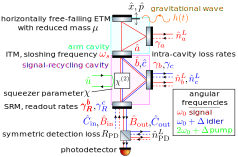
\includegraphics[angle=-90,width=0.8\textwidth]{nIS_config.pdf}
	\caption{Nondegenerate internal squeezing configuration simplified from Fig.~\ref{fig:nIS_mode_diagram} for modelling. All modes and losses are explained in the text. I simplify the arm cavities in Fig.~\ref{fig:nIS_mode_diagram} into a single cavity that represents the single-mode approximation to the differential mode $\hat a$.}
	\label{fig:nIS_config}
\end{figure}

I model nondegenerate internal squeezing using the Hamiltonian method from Section~\ref{sec:Hamiltonian_modelling} which was also used to model the results for degenerate internal squeezing in Section~\ref{sec:dIS_results}~\cite{korobkoQuantumExpanderGravitationalwave2019} and stable optomechanical filtering in Ref.~\cite{liBroadbandSensitivityImprovement2020}. %, in particular, this model combines the nondegenerate OPO model in Section~\ref{sec:nOPO} and the ~\ref{sec:dIS_model}, respectively.
% There are no steps in this derivation that have not already appeared in this thesis\jam{(check this)}.
% This model is based on and verified against the lossless model for the optomechanical analogue in Ref.~\cite{liBroadbandSensitivityImprovement2020} which effectively couples an arm cavity mode to the nondegenerate OPO model in Section~\ref{sec:nOPO}. %, and to that model I add intra-cavity and detection losses.
%\jam{(Probably need to talk about my methodology more -- state that this derivation presented is the last of a long curve of increasing complexity (more losses, radiation pressure, pump phase, etc.) and that I have verified at each stage that the model recovers the previous model. This allowed me to also consider the impact of each subsequent addition in isolation. Moreover, I should re-emphasise that it reduces to the lossless case in Li and follows the same path as the verified models of dIS and the OPOs. The point is that this derivation is not controversial.)}
When deriving my model, my approach was to start with the lossless model for the optomechanical analogue in Ref.~\cite{liBroadbandSensitivityImprovement2020} and progressively add the complexities of optical loss in each mode, pump phase, and radiation pressure so that I could study each complication separately. At each stage, I verified that the model recovered the previous stage in the appropriate limits. For brevity, I now present the complete model.

Let the modes be labelled as shown in Fig.~\ref{fig:nIS_config}. 
Here, I assume a single-mode approximation to the light in the arm cavities such that the detector in Fig.~\ref{fig:nIS_mode_diagram} is simplified to a three-mirror coupled cavity system between a single ``arm'' cavity, with resonant mode as the differential mode $\hat a$ of the detector, and the signal-recycling cavity~\footnote{The laser source and the power-recycling cavity are abstracted into the fixed circulating power in the arm cavity.}. This ``coupled-cavity'' approximation is common in the literature~\cite{adyaQuantumEnhancedKHz2020,liBroadbandSensitivityImprovement2020,miaoEnhancingBandwidthGravitationalWave2015}, was used in the degenerate internal squeezing model in Section~\ref{sec:dIS}~\cite{korobkoQuantumExpanderGravitationalwave2019}, and is valid below one ``free spectral range'' of the arm cavities (e.g.\ below 37.5~kHz for 4~km arms~\cite{miaoEnhancingBandwidthGravitationalWave2015}).
To the nondegenerate OPO model in Section~\ref{sec:nOPO}, I add the differential arm cavity mode $\hat a$ at carrier frequency $\omega_0$ with an intra-cavity loss port with transmissivity $T_{l,a}$ into vacuum $\hat n^L_a$, and detection loss $R_\text{PD}$ into vacuum $\hat n^L_\text{PD}$ modelled using the beamsplitter convention from Fig.~\ref{fig:beamsplitter_loss}~\footnote{I assume that the detection loss $R_\text{PD}$ is symmetric between the signal and idler.}. Let the gravitational-wave signal $h(t)$ from Section~\ref{sec:gravWaves} be coupled to the arm cavity mode by the test mass mechanical mode given by displacement $\hat x$ and momentum $\hat p$ (approximated as free-falling horizontally as explained in Section~\ref{sec:qnoise_GW_IFO}).
The \emph{Hamiltonian} of this system is $\hat H = \hat H_0 + \hat H_I + \hat H_\gamma + \hat H_\text{GW+RP}$ where~\cite{liBroadbandSensitivityImprovement2020} 
\begin{align}\label{eq:nIS_Hamiltonian}
\hat H_0 &= \hbar \omega_0 \hat a^\dag \hat a + \hbar \omega_0 \hat b^\dag \hat b+ \hbar (\omega_0+\Delta) \hat c^\dag \hat c + \hbar (2\omega_0+\Delta) \hat u^\dag \hat u\\
\hat H_I &= i\hbar\omega_s(\hat a\hat b^\dag-\hat a^\dag\hat b) + \hbar \frac{g}{2} (\hat u \hat b^\dag \hat c^\dag+\hat u^\dag \hat b \hat c) \nonumber\\
\hat H_\gamma &= i\hbar \sqrt{2}\int \biggl( \sqrt{\gamma_a}\left(\hat{a}^\dag(\Omega)\hat n^L_a(\Omega)-\hat{a}(\Omega)\hat{n}^{L\dag}_a(\Omega)\right) \nonumber\\
& \hspace*{1.55cm} + \sqrt{\gamma^b_R}\left(\hat{b}^\dag(\Omega)\hat{B}_\text{in}(\Omega)-\hat{b}(\Omega)\hat{B}_\text{in}^\dag(\Omega)\right) + \sqrt{\gamma_b}\left(\hat{b}^\dag(\Omega)\hat n^L_b(\Omega)-\hat{b}(\Omega)\hat{n}^{L\dag}_b(\Omega)\right) \nonumber \\
& \hspace*{1.55cm} + \sqrt{\gamma^c_R}\left(\hat{c}^\dag(\Omega)\hat C_\text{in}(\Omega)-\hat{c}(\Omega)\hat C_\text{in}(\Omega)\right) + \sqrt{\gamma_c}\left(\hat{c}^\dag(\Omega)\hat n^L_c(\Omega)-\hat{c}(\Omega)\hat{n}^{L\dag}_c(\Omega)\right)\biggr)\text{d}\Omega \nonumber\\
\hat H_\text{GW+RP} &= -\alpha (\hat{x}-L_\mathrm{arm}h(t))\left(\frac{\hat{a}+\hat{a}^\dag}{\sqrt{2}}\right)+\frac{1}{2\mu}\hat{p}^2.\nonumber
\end{align}
Here, $\alpha=\sqrt{\frac{2 P_\text{circ} \omega_0 \hbar}{c  L_\text{arm}}}$ is the coupling strength to the gravitational-wave signal~\cite{liBroadbandSensitivityImprovement2020}~\footnote{I use the value of $\alpha$ from Ref.~\cite{liBroadbandSensitivityImprovement2020} which is $\sqrt2$ more than the convention used in Ref.~\cite{korobkoQuantumExpanderGravitationalwave2019} for example.\jam{(I use the Li value for comparison to sWLC but this affects the feasibility of nIS, which value is correct? not sure, just cite)}}, $\mu=M/4$ is the ``reduced'' mass\jam{(explain)} of the test masses of mass $M$, and $\omega_s\approx c\sqrt{\frac{T_\text{ITM}}{4 L_\text{arm} L_\text{SRM}}}$ is an approximation of the sloshing frequency between the coupled cavities (also known as the coupled cavity pole) which holds when $\omega_s$ (e.g.\ 5~kHz) is below one free spectral range of the arm cavities (e.g.\ 37.5~kHz)~\cite{korobkoQuantumExpanderGravitationalwave2019}.
Of these terms in the Hamiltonian, $\hat H_0$ describes the decoupled optical system, $\hat H_I$ describes the interaction between the optical modes including the same nondegenerate squeezing as Section~\ref{sec:nOPO}, $\hat H_\gamma$ describes the input/output coupling through the readout and loss ports, and $\hat H_\text{GW+RP}$ describes the coupling of the arm cavity mode to the gravitational-wave signal and the evolution of the test mass mechanical mode due to radiation pressure~\footnote{A more natural formulation of $\hat H_\text{GW+RP}$ couples the gravitational-wave strain to the mirror position and the mirror position to the cavity mode, as shown in Fig.~\ref{fig:nIS_mode_diagram}, but the formula that I use is equivalent~\cite{bowen2015quantum}.}.
As shown in Fig.~\ref{fig:nIS_config}, there is vacuum entering the system into each intra-cavity mode $\hat n^L_a, \hat n^L_b, \hat n^L_c$, at the readout port $\hat B_\text{in}, \hat C_\text{in}$, and in the detection chain $\hat n^L_\text{PD}$ (which will be included later). Only the vacuum entering the readout port was present in the lossless model in Ref.~\cite{liBroadbandSensitivityImprovement2020}.

The \emph{Heisenberg-Langevin equations-of-motion} for this system can be found using the bosonic commutation relations, the canonical commutation relation $[\hat x,\hat p]=i\hbar$, and with all other commutators zero. As in Section~\ref{sec:nOPO}, I (1) make semi-classical and no-pump-depletion approximations that are valid below threshold to simplify the pump mode $\hat u\mapsto u e^{i\phi}=2\chi/g e^{i\phi}$, (2) enter the Interaction Picture to ignore the decoupled evolution from $\hat H_0$, and (3) take fluctuating components of each operator implicitly in the notation $\delta\hat{Q}(t)\mapsto\hat{Q}$ because it does not change the equations-of-motion\jam{(is this true? it is not clear to me)}. I find the equations-of-motion to be\jam{(change notation to be clearer, e.g.\ $\gamma_{b,\text{tot}}=\gamma_{b,R}+\gamma_{b,l}$?)}
\begin{equation}\label{eq:nIS_EoM}
\begin{cases}
\dot{\hat{a}}=-\omega_s\hat{b} - \gamma_a \hat{a} + \sqrt{2\gamma_a}\hat{n}^L_a+\frac{i}{\hbar}\alpha(\hat{x}-L_\mathrm{arm}h)\frac{1}{\sqrt{2}}\\
\dot{\hat{b}}=\omega_s\hat{a} - i\chi e^{i\phi}\hat{c}^\dagger - \gamma^b_\mathrm{tot} \hat{b} + \sqrt{2\gamma^b_R}\hat{B}_\mathrm{in} + \sqrt{2\gamma_b}\hat{n}^L_b\\
\dot{\hat{c}}=-i\chi e^{i\phi}\hat{b}^\dagger - \gamma^c_\mathrm{tot} \hat{c} + \sqrt{2\gamma^c_R}\hat{C}_\mathrm{in} + \sqrt{2\gamma_c}\hat{n}^L_c\\
\dot{\hat{x}}=\frac{1}{\mu}\hat{p}\\
\dot{\hat{p}}=\alpha\left(\frac{\hat{a}+\hat{a}^\dag}{\sqrt{2}}\right).
\end{cases}
\end{equation}
I solve these equations in the \emph{Fourier domain}. As in Section~\ref{sec:nOPO}, let $\vec{\hat d}(\Omega)=(\hat b(\Omega), \hat b^\dag(-\Omega), \hat c(\Omega), \hat c^\dag(-\Omega))^\text{T}$, where I use the compact notation $\tilde{\delta\hat{Q}}(\Omega)\mapsto\hat{Q}(\Omega)$ for the Fourier transform of each mode, with similar signal-idler vectorisation for each signal and idler mode, e.g.\ $\vec{\hat{D}}_\text{in}(\Omega),\; \vec{\hat n}^L_d(\Omega)$~\footnote{Where the notation $d$ indicates a similar vector to $\vec{\hat d}(\Omega)$ of both quadratures of the signal and idler.}. Let $\vec h(\Omega)=\tilde h(\Omega) (1,1,0,0)^\text{T}$ (since $h(t)$ is real, $\tilde h(\Omega)=\tilde h(-\Omega)^*$), $\vec{\hat a}(\Omega)=(\hat a(\Omega), \hat a^\dag(-\Omega),0,0)^\text{T}$~\footnote{I substitute $\hat x(\Omega) = \frac{-\alpha}{\mu\Omega^2\sqrt2}\left(\hat{a}(\Omega)+\hat{a}^\dag(-\Omega)\right)$, found by Fourier transforming Eq.~\ref{eq:nIS_EoM}, in the equation for $\hat a(\Omega)$ before vectorising.}, and similarly for $\vec{\hat n}^L_a(\Omega)$.
By Fourier transforming, vectorising, and then solving the resulting linear algebraic equations for $\vec{\hat d}(\Omega)$ using a similar process to Section~\ref{sec:Hamiltonian_modelling}, I find that the signal and idler intra-cavity modes, in terms of each vacuum input and the gravitational-wave signal, are
\begingroup
\allowdisplaybreaks
\begin{align}\label{eq:nIS_vecb}
\vec{\hat{d}}(\Omega)&= \mathrm{M}_d^{-1}\Biggl(\omega_s\begin{bsmallmatrix}
1 &  &  &  \\
 & 1 &  &  \\
 &  & 0 &  \\
 &  &  & 0
\end{bsmallmatrix}\mathrm{M}_a^{-1}\left(\sqrt{2\gamma_a}\begin{bsmallmatrix}
1 &  &  &  \\
 & 1 &  &  \\
 &  & 0 &  \\
 &  &  & 0
\end{bsmallmatrix}\vec{\hat{n}}^L_a(\Omega)-i\beta\begin{bsmallmatrix}
1 &  &  &  \\
 & -1 &  &  \\
 &  & 0 &  \\
 &  &  & 0
\end{bsmallmatrix}\vec{h}(\Omega)\right)\\&\hspace{1.4cm}+ \sqrt{2}\begin{bsmallmatrix}
\sqrt{\gamma^b_R} &  &  &  \\
 & \sqrt{\gamma^b_R} &  &  \\
 &  & \sqrt{\gamma^c_R} &  \\
 &  &  & \sqrt{\gamma^c_R}
\end{bsmallmatrix}\vec{\hat D}_\mathrm{in}(\Omega) + \sqrt{2}\begin{bsmallmatrix}
\sqrt{\gamma_b} &  &  &  \\
 & \sqrt{\gamma_b} &  &  \\
 &  & \sqrt{\gamma_c} &  \\
 &  &  & \sqrt{\gamma_c}
\end{bsmallmatrix}\vec{\hat n}^L_d(\Omega)\Biggr)\nonumber\\
\mathrm{M}_a &= (\gamma_a-i\Omega)\mathrm{I}+\frac{i\rho}{\Omega^2 \sqrt{2}}\begin{bsmallmatrix}
1 & 1 &  &  \\
-1 & -1 &  &  \\
 &  & 0 &  \\
 &  &  & 0
\end{bsmallmatrix}\\
\text{M}_d&=\begin{bsmallmatrix}
\gamma^b_\mathrm{tot} &  &  &  \\
 & \gamma^b_\mathrm{tot} &  &  \\
 &  & \gamma^c_\mathrm{tot} &  \\
 &  &  & \gamma^c_\mathrm{tot} 
\end{bsmallmatrix}-i\Omega \text{I}+\chi \begin{bsmallmatrix}
0 &  &  & i e^{i\phi} \\
 & 0 & -i e^{-i\phi} &  \\
 & i e^{i\phi} & 0 &  \\
-i e^{-i\phi} &  &  & 0
\end{bsmallmatrix}+\omega_s^2\begin{bsmallmatrix}
1 &  &  &  \\
 & 1 &  &  \\
 &  & 0 &  \\
 &  &  & 0
\end{bsmallmatrix}\text{M}_a^{-1}\begin{bsmallmatrix}
1 &  &  &  \\
 & 1 &  &  \\
 &  & 0 &  \\
 &  &  & 0
\end{bsmallmatrix}.
\end{align}
\endgroup
Here, $\text{I}$ is the 4-by-4 identity matrix, all off-diagonal terms in each 4-by-4 matrix are zero unless otherwise shown, and the re-scaled coupling constants for the gravitational-wave signal and the radiation pressure~\footnote{Here, $\rho=0$, i.e.\ $\mu=M/4\rightarrow\infty$, turns off the radiation pressure noise.}, respectively, are
\begin{equation}\label{eq:beta_and_rho}
\beta = \frac{\alpha L_\mathrm{arm}}{\sqrt{2}\hbar}=\sqrt{\frac{ P_\text{circ}L_\text{arm} \omega_0 }{c  \hbar}},\quad \rho = \frac{\alpha^2}{\sqrt{2}\hbar\mu}=\frac{\sqrt{2} P_\text{circ} \omega_0}{c \mu L_\text{arm}}.
\end{equation}
Using the input/output relation at the readout port like in Eq.~\ref{eq:dOPO_IO}, the beamsplitter model of detection loss ($R_\text{PD}$) in the output field ($\hat{B}_\text{out}, \hat{C}_\text{out}$), and $\Gamma= \frac{1}{\sqrt2}\begin{bsmallmatrix}
1 & 1 &  &  \\
-i & i &  &  \\
 &  & 1 & 1 \\
 &  & -i & i
\end{bsmallmatrix}$ to convert to quadratures, I find the \emph{signal and idler quadratures at the photodetector}~\footnote{Here, $\vec{\hat X}(\Omega)=(\hat X_{b,1}(\Omega),\hat X_{b,2}(\Omega),\hat X_{c,1}(\Omega),\hat X_{c,2}(\Omega))^\text{T}$, as in Section~\ref{sec:nOPO}.} to be
\begin{align}
\label{eq:nIS_IO}
\vec{\hat X}_\mathrm{PD}(\Omega)&=\sqrt{1-R_\text{PD}}\vec{\hat X}_\mathrm{in}(\Omega)+\sqrt{R_\text{PD}}\vec{\hat X}^L_\text{PD}(\Omega)-\sqrt{2(1-R_\text{PD})}\Gamma\begin{bsmallmatrix}
\sqrt{\gamma^b_R} &  &  &  \\
 & \sqrt{\gamma^b_R} &  &  \\
 &  & \sqrt{\gamma^c_R} &  \\
 &  &  & \sqrt{\gamma^c_R}
\end{bsmallmatrix}\vec{\hat d}(\Omega).
\end{align}
Substituting Eq.~\ref{eq:nIS_vecb} into Eq.~\ref{eq:nIS_IO} and using $\Gamma$ to convert the remaining vacuum inputs to quadratures, e.g.\ $\vec{\hat{n}}^L_a(\Omega)$ to $\Gamma^{-1}\vec{\hat X}^L_a(\Omega)$, I find the output quadratures at the photodetector in terms of the input quadratures and the gravitational-wave signal to be
\begingroup
\allowdisplaybreaks
\begin{align}\label{eq:nIS_Xpd}
\vec{\hat X}_\mathrm{PD}(\Omega)&=\text{T}\vec h(\Omega)+\text{R}_\text{in}\vec{\hat X}_\mathrm{in}(\Omega)+\text{R}^L_a\vec{\hat X}^L_a(\Omega)+\text{R}^L_b\vec{\hat X}^L_b(\Omega)+\text{R}^L_\text{PD}\vec{\hat X}^L_\text{PD}(\Omega)\\
\text{T}&=-\sqrt{1-R_\text{PD}}\omega_s(-i\beta)\Gamma \sqrt{2}\begin{bsmallmatrix}
\sqrt{\gamma^b_R} &  &  &  \\
 & \sqrt{\gamma^b_R} &  &  \\
 &  & \sqrt{\gamma^c_R} &  \\
 &  &  & \sqrt{\gamma^c_R}
\end{bsmallmatrix}\text{M}_d^{-1}\begin{bsmallmatrix}
1 &  &  &  \\
 & 1 &  &  \\
 &  & 0 &  \\
 &  &  & 0
\end{bsmallmatrix}\text{M}_a^{-1}\begin{bsmallmatrix}
1 &  &  &  \\
 & -1 &  &  \\
 &  & 0 &  \\
 &  &  & 0
\end{bsmallmatrix}\\
\text{R}_\text{in}&=\sqrt{1-R_\text{PD}}\Gamma\left(\text{I}-2\begin{bsmallmatrix}
\sqrt{\gamma^b_R} &  &  &  \\
 & \sqrt{\gamma^b_R} &  &  \\
 &  & \sqrt{\gamma^c_R} &  \\
 &  &  & \sqrt{\gamma^c_R}
\end{bsmallmatrix}\text{M}_d^{-1}\begin{bsmallmatrix}
\sqrt{\gamma^b_R} &  &  &  \\
 & \sqrt{\gamma^b_R} &  &  \\
 &  & \sqrt{\gamma^c_R} &  \\
 &  &  & \sqrt{\gamma^c_R}
\end{bsmallmatrix}\right)\Gamma^{-1}\\
\text{R}^L_a&=-\sqrt{1-R_\text{PD}}\omega_s\Gamma 2\sqrt{\gamma_a}\begin{bsmallmatrix}
\sqrt{\gamma^b_R} &  &  &  \\
 & \sqrt{\gamma^b_R} &  &  \\
 &  & \sqrt{\gamma^c_R} &  \\
 &  &  & \sqrt{\gamma^c_R}
\end{bsmallmatrix}\text{M}_d^{-1}\begin{bsmallmatrix}
1 &  &  &  \\
 & 1 &  &  \\
 &  & 0 &  \\
 &  &  & 0
\end{bsmallmatrix}\text{M}_a^{-1}\begin{bsmallmatrix}
1 &  &  &  \\
 & 1 &  &  \\
 &  & 0 &  \\
 &  &  & 0
\end{bsmallmatrix}\Gamma^{-1}\\
\text{R}^L_b&=-\sqrt{1-R_\text{PD}}\Gamma 2\begin{bsmallmatrix}
\sqrt{\gamma^b_R} &  &  &  \\
 & \sqrt{\gamma^b_R} &  &  \\
 &  & \sqrt{\gamma^c_R} &  \\
 &  &  & \sqrt{\gamma^c_R}
\end{bsmallmatrix}\text{M}_d^{-1}\begin{bsmallmatrix}
\sqrt{\gamma^b_R} &  &  &  \\
 & \sqrt{\gamma^b_R} &  &  \\
 &  & \sqrt{\gamma^c_R} &  \\
 &  &  & \sqrt{\gamma^c_R}
\end{bsmallmatrix}\Gamma^{-1}\\
\text{R}^L_\text{PD}&=\sqrt{R_\text{PD}} \text{I}.
\end{align}
\endgroup
The \emph{total quantum noise} is given by the spectral density matrix Eq.~\ref{eq:total_noise_matrix}, which simplifies, assuming uncorrelated vacuum at each loss port, to
\begin{equation}\label{eq:nIS_Sx}
\text{S}_X=\text{R}_\text{in}\text{R}_\text{in}^\dag+\text{R}^L_a{\text{R}^L_a}^\dag+\text{R}^L_b{\text{R}^L_b}^\dag+\text{R}^L_\text{PD}{\text{R}^L_\text{PD}}^\dag.
\end{equation} % same expression as dIS
The structure of $\text{S}_X$ is divided into 2-by-2 blocks of signal-signal, signal-idler, and idler-idler (co)variances as in Section~\ref{sec:nOPO} but now with terms for the radiation-pressure noise such that the variances and covariances no longer reduce to 1 and 0, respectively, when the squeezer is off. The pump phase only appears in the off-diagonal, signal-idler covariances.

The \emph{signal response} for a given quadrature is defined with respect to the signal $\tilde h(\Omega)$, not $\vec h(\Omega)$, and therefore the vector of the signal response for each signal and idler quadrature at the photodetector is
\begin{equation}\label{eq:nIS_sigRO_signal_response}
\text{T}\begin{psmallmatrix}1 \\1\\0\\0\end{psmallmatrix} = \frac{2 \beta \sqrt{1-R_\text{PD}} \omega_s}{(\gamma_a-i \Omega ) \left(\chi ^2-(\gamma^b_\text{tot}-i\Omega) (\gamma^c_\text{tot}-i\Omega)\right)-\omega_s^2 (\gamma^c_\text{tot}-i \Omega )} \begin{psmallmatrix}0 \\-\sqrt{\gamma^b_R}(\gamma^c_\text{tot}-i\Omega)\\\sqrt{\gamma^c_R}\chi\cos(\phi)\\\sqrt{\gamma^c_R}\chi\sin(\phi)\end{psmallmatrix}.
\end{equation}
Here, $\text{T}\vec h(\Omega)=\text{T}\begin{psmallmatrix}1 \\1\\0\\0\end{psmallmatrix}\tilde h(\Omega)$ gives the signal in each quadrature.
Therefore, by Eq.~\ref{eq:nIS_sigRO_signal_response}, the gravitational-wave signal is in the second signal quadrature as well as each idler quadrature when the squeezer is on ($\chi\neq0$). For simplicity and to compare to Ref.~\cite{liBroadbandSensitivityImprovement2020}, I will consider measuring the second signal quadrature, henceforth referred to as ``signal readout''. However, this is not necessarily the optimum readout of the signal quadratures since the noise might be sufficiently lower in the first quadrature to preference measuring some quadrature between the two. I will consider this and alternative readout schemes involving the idler in Chapter~\ref{chp:idler_readout}.

The quantum noise and signal responses of the signal readout scheme are, respectively, $\sqrt{(\text{S}_X)_{2,2}}$ and $\abs{\left(\text{T}\begin{psmallmatrix}1 \\1\\0\\0\end{psmallmatrix}\right)_2}$, and the \emph{sensitivity}, conventionally plotted as the noise-to-signal ratio, is
\begin{equation}\label{eq:nIS_sigRO_sens}
\sqrt{S_h} = \frac{\sqrt{(\text{S}_X)_{2,2}}}{\abs{\left(\text{T}\begin{psmallmatrix}1 \\1\\0\\0\end{psmallmatrix}\right)_2}}.
\end{equation}
% verified these results by repeating the model with 2x2 matrices and 4x4 matrices, important to mention this because it is part of the methodology
To partially validate this result, I have repeated its derivation using 2-by-2 matrices~\footnote{Which is not a physically meaningful difference, and therefore I will not present it here, but it separates the signal and idler such that the derivations are not identical.}, and will compare it to the known limits below. %in Section~\ref{sec:nOPO_reduction}.


\section{Results}
\label{sec:nIS_sigRO_results}

\begin{table}
\centering
% \begin{tabular}{@{}ll|ll@{}}
% \toprule
% carrier wavelength, $\lambda_0$ & 2 $\mu\text{m}$ & signal mode transmissivity, $T_{\text{SRM},b}$ & 0.046 \\
% arm cavity length, $L_\text{arm}$ & 4 km & signal readout rate, $\gamma^b_R$ & 500 Hz \\
% signal-recycling cavity length, $L_\text{SRC}$ & 1.124 km & idler mode transmissivity, $T_{\text{SRM},c}$ & 0 \\
% circulating arm power, $P_\text{circ}$ & 3 MW & idler readout rate, $\gamma^c_R$ & 0 Hz \\
% test mass mass, $M$ & 200 kg & arm intra-cavity loss, $T_{l,a}$ & 100 ppm \\
% radiation pressure, $\rho$ & $\neq0$ & signal mode intra-cavity loss, $T_{l,b}$ & 1000 ppm \\
% input test mass transmissivity, $T_\text{ITM}$ & 0.197 & idler mode intra-cavity loss, $T_{l,c}$ & 1000 ppm \\
% sloshing frequency, $\omega_s$ & 5 kHz & detection loss, $R_\text{PD}$ & $10\%$ \\ \bottomrule
% \end{tabular}
\begin{tabular}{@{}ll|ll@{}}
\toprule
signal-recycling cavity length, $L_\text{SRC}$ & 1.124 km & signal mode transmissivity, $T_{\text{SRM},b}$ & 0.046 \\
input test mass transmissivity, $T_\text{ITM}$ & 0.197 & signal readout rate, $\gamma^b_R$ & 500 Hz \\
sloshing frequency, $\omega_s$ & 5 kHz & idler mode transmissivity, $T_{\text{SRM},c}$ & 0 \\
idler mode intra-cavity loss, $T_{l,c}$ & 1000 ppm & idler readout rate, $\gamma^c_R$ & 0 Hz \\ \bottomrule
\end{tabular}
\caption{Nondegenerate internal squeezing signal readout parameter set is based on LIGO~Voyager~\cite{LIGO_Voyager} and the same as Table~\ref{tab:dIS_parameters} but with the deviations shown to make the sensitivity more sharply peaked ($\gamma^b_R$ is now 0.5~kHz compared to 5~kHz) and the addition of the idler mode. Radiation pressure is included using $\rho\neq0$ from Eq.~\ref{eq:beta_and_rho} unless $\rho=0$ is stated. The results shown use these parameters unless stated otherwise.}
\label{tab:signal_RO_parameters}
\end{table}

I now examine some of the immediate results of the model: (1) the lossless behaviour of the system, (2) the general behaviour when losses are introduced, and (3) the high arm loss limit.
% (1) the general features of the signal and noise responses and sensitivity, (2) the reduction to known models in certain loss limits, and (3) the stability of the system.
Throughout the rest of this thesis, I will use the parameter set in Table~\ref{tab:signal_RO_parameters}. The choice of parameter set can bias the analysis of a configuration, and I mention, where relevant, the effects of varying the parameters (e.g.\ the readout rates which have a large variation in the literature~\cite{liBroadbandSensitivityImprovement2020,miaoDesignGravitationalWaveDetectors2018,korobkoQuantumExpanderGravitationalwave2019}). These parameters have not been optimised for the sensitivity which I leave to future work. % parameter set. % from Section~\ref{sec:dIS_results}, in particular, I will use the  unless stated otherwise.

% \subsubsection{Lossless limit}
\label{sec:nIS_lossless_limit}

\begin{figure}
    \centering
    \includegraphics[width=\textwidth]{nIS_lossless.pdf}
    \caption{Nondegenerate internal squeezing in the lossless limit, showing the quantum noise (upper-left panel), signal response (bottom-left panel), and sensitivity (right panel) with squeezing (red curves) and without squeezing (blue curves). I also show the results with ($\rho\neq0$, see Eq.~\ref{eq:beta_and_rho}) and without ($\rho=0$) radiation pressure noise, and I compare them to the lossless optomechanical analogue from Section~\ref{sec:sWLC} (cyan curve) with the same ratio to threshold. I use the data from Fig.~5 in Ref.~\cite{liBroadbandSensitivityImprovement2020} with permission from the authors~\cite{xiangLiPersonalCommunication}. The noise and signal responses and sensitivity reduce to the expected lossless limit. I use the parameters in Table~\ref{tab:signal_RO_parameters} but with no losses.}
    \label{fig:nIS_lossless}
\end{figure}

To partially validate the model, I check that it reduces to the expected \emph{lossless limit} in Fig.~\ref{fig:nIS_lossless}.
In the lossless limit, where $\gamma_a=\gamma_b=\gamma_c=R_\text{PD}=0$, the equations-of-motion of nondegenerate internal squeezing in Eq.~\ref{eq:nIS_EoM} reduce to those of the lossless optomechanical analogue in Ref.~\cite{liBroadbandSensitivityImprovement2020}~\footnote{Compare $\hat H_I$ from Eq.~\ref{eq:sWLC_HI} to Eq.~\ref{eq:nIS_Hamiltonian} with the semi-classical approximation to the pump mode $\hat u$.}. The resulting noise and signal responses and sensitivity also reduce to this limit as shown in Fig.~\ref{fig:nIS_lossless}. This limit is expected from the comparison of the mode structure of the two lossless systems discussed in Section~\ref{sec:modal_equivalence}.
% this is because of the use of alpha from Li and not Korobko 
% no losses means no antisqueezing of shot noise but yes RPN, why? threshold=0 problem?

The \emph{general behaviour of nondegenerate internal squeezing without losses} is shown in Fig.~\ref{fig:nIS_lossless}. %I examine the signal and noise responses separately to understand the sensitivity.
With the squeezer off, the sensitivity curve is shaped by the radiation-pressure noise below 10~Hz and the signal response resonance at the sloshing frequency 5~kHz with bandwidth 500~Hz determined by the signal readout rate $\gamma^b_R$, as discussed in Section~\ref{sec:dIS_results}.
With the squeezer on, lossless nondegenerate internal squeezing (1) amplifies the radiation-pressure noise to dominate below 100~Hz and further amplifies it with increased squeezer parameter and (2) amplifies the signal response from DC up to the peak frequency. The peak frequency without squeezing is at the sloshing frequency but decreases with increased squeezer parameter which is related to the squeezing threshold and will be discussed later.
The signal response is amplified by the white-light cavity effect similarly to the optomechanical analogue in Section~\ref{sec:sWLC}. %, i.e.\ the resonance behaviour of the coupled cavity system is changed by introducing the idler mode\jam{(is this true? I am not sure. the signal response still falls off at the same rate so bandwidth doesn't seem to improve except by the LF amplification?)}.
The changes are not localised to the sloshing frequency, e.g.\ the radiation-pressure noise is anti-squeezed, unlike degenerate internal squeezing, because coupling to the idler mode changes the response of the detector.
% Therefore, the radiation pressure noise at ``low'' frequencies can be affected and is also anti-squeezed.\jam{(why is it amplified, happens in lossless case as well? why does the other quadrature appear now? is it worsened proportionally to the pump power?)}


% \subsubsection{General lossy behaviour}
\label{sec:nIS_general_behaviour}
% should this be down in results section? --> this is a results chapter, maybe include a short section discussing the general performance (separate from the science case analysis in chapter 5?)

% plot: classic N, S, NSR; also noise budget plot
% need to show some example plots here to set up those in the next section?
\begin{figure}
	\centering
	\includegraphics[width=\textwidth]{nIS_N_S_NSR.pdf}
	\caption{Nondegenerate internal squeezing with all the optical losses included, showing the noise (upper-left panel), signal (bottom-left panel), and sensitivity (right panel). The effect of the squeezer and the radiation pressure noise (turned off by setting $\rho=0$) on the sensitivity are shown; the squeezer anti-squeezes the noise around the peak frequency of the signal response. The losses change the slope of the radiation pressure noise around 10~Hz and also cause the signal to not be amplified down to DC compared to the lossless case in Fig.~\ref{fig:nIS_lossless}. The squeezer parameter is normalised to the lossy threshold which will be found later. I use the parameters in Table~\ref{tab:signal_RO_parameters}.}
	\label{fig:nIS_general_sens}
\end{figure}

% analyse typical nIS plot features before getting into different tests
The \emph{general lossy behaviour} of nondegenerate internal squeezing is shown in Fig.~\ref{fig:nIS_general_sens}. 
The behaviour with losses is the same as the lossless case in Fig.~\ref{fig:nIS_lossless} except that (1) the shot noise is anti-squeezed around the peak frequency\jam{(why?)}, (2) the radiation-pressure noise is anti-squeezed less, and (3) the signal amplification drops off below 100~Hz and converges to the response without squeezing below 10~Hz\jam{(explain why?)}. The bandwidth of the signal amplification is determined by the losses and therefore does not extend to DC with losses present\jam{(check. why?)}. The peak frequency around which the signal and shot noise are amplified is determined by the squeezer parameter, sloshing frequency, and loss rates.
Like the signal, the shot noise is also anti-squeezed around the peak frequency because the internal squeezer affects both the signal and noise. %, but the noise is not anti-squeezed in the lossless limit because\jam{... (why? I do not know.)}.
Inspecting the limit of smaller and smaller losses confirms that the shot noise peak decreases until it vanishes in the lossless limit as expected by analogy to the optomechanical configuration~\cite{liBroadbandSensitivityImprovement2020}.
% With the squeezer turned on, (1) the shot noise is anti-squeezed around the peak frequency determined by the squeezer parameter, sloshing frequency, and loss rates; (2) the radiation-pressure noise is anti-squeezed to now dominate below 100~Hz; and (3) the signal is amplified around the same frequency as the shot noise and at frequencies down to 10~Hz, below which it converges to the value without squeezing due to losses. 
Overall, the squeezer now improves sensitivity from around 40--3000~Hz and worsens it outside that band except above 10~kHz where the sensitivity is the same without squeezing. This is largely the same behaviour as the lossless case, but I will more closely examine the effects of each loss in the next chapter.
These quoted frequencies are specific to this parameter set but the general performance is the same: nondegenerate internal squeezing improves sensitivity at some broad range of ``middle'' frequencies at the cost of ``low'' frequency sensitivity. 
% Some of these effects will be explained later, e.g.\ the frequency around which the shot noise and the signal peak are amplified is determined by the threshold of the system, but some of these results can be explained immediately.
 % and the effect of losses will be left until I consider gravitational-wave detection feasibility.
% changing the signal response via the white-light cavity effect?
% why aren't the changes local to the sloshing frequency, like dIS?

% The changes are not localised to the sloshing frequency unlike degenerate internal squeezing in Section~\ref{sec:dIS_results}\jam{(check this, shouldn't this mean that they are still expected around the coupling frequencies?)}. 
%In the simple explanation of the signal-recycling cavity reflecting the light back into the arms to experience the gravitational wave more, the addition of the idler mode, which is not directly coupled to the arms or measured, somehow\jam{(how/why? this is wishy-washy)}.
% why does radiation pressure noise worsen?
% ~\footnote{I only talk about the radiation pressure noise where it is dominant, i.e.\ at ``low'' frequencies below the Standard Quantum Limit\jam{(is this necessary to say?)}}

% To understand how the radiation pressure noise is affected, I consider how it appears in each of the contributions to the total quantum noise, shown in Fig.~\ref{fig:nIS_sigRO_noise_budget}. The radiation pressure noise appears in the contribution from the readout port and each intra-cavity loss port because these noises are coupled indirectly to the arm mode, unlike the detection loss which therefore has only shot noise. In particular, opening the idler readout port introduces more vacuum and turning the squeezer on indirectly couples the idler mode and this noise into the signal readout, which is why radiation pressure noise worsens by turning the squeezer on even when there are no losses\jam{(check this)}, which will be shown later in Fig.~\ref{fig:nIS_lossless}.\jam{(why is the shot noise not amplified at LF?)}
% This is because the radiation pressure noise, with the gravitational-wave signal, enters the measured, second signal quadrature after the input test mass. Having already seen the arm cavity loss, it gets added here to each of the noises that travel through the signal mode\jam{(what am I trying to say?)}. It is then anti-squeezed\jam{(check this)} and read out.

% explain the effect of each parameter? (except leave tolerance to losses to science case chapter)
% in terms of the configuration parameters rather than derived parameters such as the sloshing frequency and readout rates
The \emph{effect of each configuration parameter} is similar to the effect on the interferometer without squeezing discussed in Sections~\ref{sec:intro_IFO} and~\ref{sec:dIS_results}. To summarise, increasing the circulating power in the arms increases the signal response at all frequencies via $\beta$ in Eq.~\ref{eq:nIS_sigRO_signal_response}. Increasing the arm length increases the same factor $\beta$ as the power but also decreases the bandwidth of the signal response and the sloshing frequency which determines the peak. The sloshing frequency also decreases with decreased input test mass transmission and longer signal-recycling cavities. Increasing the signal-recycling length decreases the bandwidth of the signal peak~\footnote{The arm cavity bandwidth gives the overall shape of the signal response but the signal-recycling cavity bandwidth gives the width of the peak at the sloshing frequency.}, which is also decreased by decreased signal-recycling mirror transmission. The radiation-pressure noise increases with lighter test masses and increased pump power. Finally, increased pump power also increases the peak shot noise and signal amplification, and the pump phase does not affect signal readout.

% \subsection{Reduction to known systems}
% show that this follows from the EoM but can be verified by looking at the plots
% I predict the behaviour by taking the limits of the equations-of-motion in Eq.~\ref{eq:nIS_EoM} and verify it by examining the plots of the noise and signal responses.

% \subsubsection{High arm loss limit}
\label{sec:nOPO_reduction}

% \begin{figure}
% 	\centering
% 	\includegraphics[width=\textwidth]{nIS_nOPO_limit.pdf}
% 	\caption{\jam{(Purpose: show limits 2/2)}\jam{(Can cut this plot and instead just claim the limit in the text.)} Nondegenerate internal squeezing shot noise response showing the high arm loss limit compared to the response from a nondegenerate OPO with the input test mass fully reflective. The signal and idler readout rates are assumed symmetric. The shot noise converges as expected.}
% 	\label{fig:nIS_signal_nOPO_limit}
% \end{figure}

% full 4x4 matrix agrees, not just variance 1,1
% give best explanation of ITM T=0, but can admit that while the maths is clear the physics is not obvious -- potentially requires more thought
To further validate the model, I check that it reduces to the expected limit when the arm loss is taken to infinity. 
In the \emph{high arm loss limit}, $\gamma_a\rightarrow\infty$, the equations-of-motion of nondegenerate internal squeezing in Eq.~\ref{eq:nIS_EoM} reduce to those in Eq.~\ref{eq:nOPO_EoM} for a nondegenerate OPO between the signal-recycling mirror and a fully-reflective input test mass.
I have verified this limit by checking that each of the terms of the shot noise matrix $\text{S}_X|_{\rho=0}$ from Eq.~\ref{eq:nIS_Sx} reduces to the OPO value~\cite{schoriNarrowbandFrequencyTunable2002}~\footnote{Moreover, I have checked that a similar limit holds for the model of degenerate internal squeezing in Section~\ref{sec:dIS} that reduces to a degenerate OPO with the input test mass fully reflective.}.\jam{(check if the QRPN vanishes)}
%, see Section~\ref{sec:dIS_optical_loss}, where the explanation for why the mirror is fully reflective is the same as that case. 
% therefore mystery of the idler loss carries over: idler loss cannot be zero
Although I expected physically that the input test mass would instead become another loss port with its original transmissivity, this behaviour can be explained as in the limit the equation-of-motion for the fluctuating component becomes $\dot{\delta\hat a}\approx -\gamma_a \delta\hat a$ which quickly decays, and, therefore, any vacuum fluctuations $\delta\hat n^L_a$ cannot couple to $\delta\hat b$. However, I suspect that this is a false consequence of the single-mode approximation and that if a ``transfer matrix'' approach (e.g.\ in Refs.~\cite{korobkoQuantumExpanderGravitationalwave2019,finesse})~\footnote{Where the fields at a point are propagated inside the cavities and the cavity modes, e.g.\ $\hat a$, are not explicit. Not to be confused with the transfer matrices describing the signal $T$ and noise $R$ responses. The Hamiltonian method is more comprehensive than this approach and could also be modified to use the fields at a point rather than the cavity modes~\cite{danilishinQuantumMeasurementTheory2012}.} was instead used then the limit would instead be a degenerate OPO with added intra-cavity loss to account for the open input test mass port; I leave verifying this to future work.
Therefore, this model predicts that lossy nondegenerate internal squeezing behaves somewhere between the lossless optomechanical analogue and the nondegenerate OPO but closer to the former since the realistic arm loss for future detectors is below this high loss regime (e.g.\ 100~ppm versus above 10000~ppm) and thus the exact behaviour in this regime is not of concern. %And so, I expect features to be inherited from these limiting configurations, e.g.\ that threshold is poorly defined when idler loss is zero should be inherited from the nondegenerate OPO.

Even further validation of this analytic model could be performed by comparing it to a numerical model, which I leave to future work.


\section{Stability and threshold}
\label{sec:stability_and_threshold}

I now determine when nondegenerate internal squeezing is stable and below threshold. %, which is required for experiments. %I will use the no-pump-depletion assumption to link when the system is marginally stable and when it is at threshold.

\subsection{Stability}
\label{sec:nIS_stability}

Stability is a feature of nondegenerate internal squeezing that might not be fully inherited from its limiting configurations. I use the same method to determine stability as degenerate internal squeezing in Appendix~\ref{app:dIS_stability}. The signal and noise responses are fractions of polynomials of $\Omega, \chi$ with denominators~\footnote{I state these for the modulus-squared responses, i.e.\ $(\text{S}_X)_{2,2}$ from Eq.~\ref{eq:nIS_Sx} and $\abs{\left(\text{T}\begin{psmallmatrix}1 \\1\\0\\0\end{psmallmatrix}\right)_2}^2$ from Eq.~\ref{eq:nIS_sigRO_signal_response}, but the poles, i.e.\ zeros of $q$, do not change under the square root.} given by $q(\Omega,\chi)$ and $\Omega^4 q(\Omega,\chi) q(\Omega,-\chi)$, respectively. Here, $q$ only depends on $\chi^2$ and so the noise response denominator is $\Omega^4 q(\Omega,\chi)^2$, where $q$ is some polynomial in $\Omega, \chi$, 
\begin{align}\label{eq:nIS_denom}
q(\Omega,\chi)&=\left(\gamma_a^2+\Omega ^2\right) \left(\Omega ^2 \left({\gamma^b_\text{tot}}^2+{\gamma^c_\text{tot}}^2+2 \chi ^2\right)+\left({\gamma^b_\text{tot}} {\gamma^c_\text{tot}}-\chi ^2\right)^2+\Omega ^4\right)\\
&-2 \omega_s^2 \left(\gamma_a {\gamma^c_\text{tot}} \chi ^2-\gamma_a {\gamma^b_\text{tot}} \left({\gamma^c_\text{tot}}^2+\Omega ^2\right)+\Omega ^2 \left({\gamma^c_\text{tot}}^2+\chi ^2+\Omega ^2\right)\right)+\omega_s^4 \left({\gamma^c_\text{tot}}^2+\Omega ^2\right).\nonumber
\end{align}
This means that the poles of the responses are the shared zeros of $q$~\footnote{The second factor of $q$ in the noise response cancels with a term in the numerator meaning that the multiplicity is the same.}, except for the radiation-pressure noise singularity at $\Omega=0$ which I ignore because it comes from the horizontally free-falling mass assumption and physically the resonance of the test mass is finite. % That the rest of the poles are shared is expected because the stability of the system should be the same for the signal and noise\jam{(should it? no?)}~\cite{}.
Therefore, nondegenerate internal squeezing is unstable if any of the complex $\Omega$ zeros of $q$ have a positive imaginary part and is marginally stable if any of them have no imaginary part~\cite{nise_2019}. As shown in Fig.~\ref{fig:nIS_stability}, the \emph{lossless system is stable below threshold} ($\chi\leq\chi_\text{thr}=\omega_s$) which agrees with Ref.~\cite{liBroadbandSensitivityImprovement2020}. The lossy system is also stable up to a point that I will shortly define to be the threshold. %The behaviour above threshold cannot be inferred using t.
% non-effect of RP, pump phase
Since Eq.~\ref{eq:nIS_denom} only depends on the pump power, readout and loss rates, and sloshing frequency, therefore, other factors, such as radiation pressure or pump phase, do not affect the stability.

% plot: imaginary part of poles
\begin{figure}[t]
    \centering
    \includegraphics[width=0.95\textwidth]{nIS_stability.pdf}
    \caption{Stability of nondegenerate internal squeezing, for lossless (left panel) and lossy (right panel) cases. I show the imaginary part of the shared poles of the noise and signal responses versus the squeezer parameter; where the imaginary part becomes positive, the system becomes unstable. The different colours indicate different poles (zeros of $q$) found numerically, and any discontinuities are numerical or plotting artefacts. I will define the singularity threshold ($\chi_\text{thr}$) such that the system is stable below threshold; the value of $\chi_\text{thr}$ is different between the two cases. I use the parameters in Table~\ref{tab:signal_RO_parameters}.}
    \label{fig:nIS_stability}
\end{figure}


\subsection{Singularity threshold}
\label{sec:singularity_threshold}
% motivate this by the previous section's looking at poles, now looking at real poles that could be encountered, to avoid confusion with the complex poles that are always present I will call these real poles ``singularities''

%\jam{(Rewrite the following as the threshold of stability, should just be one paragraph, make clear that the link to gain-loss balancing is just that if there is a net gain but no pump depletion then energy is demonstrably unpreserved and the field will grow without end which is unstable. But be honest that I do not know and that this result would be different with pump-depletion added.)}

%\jam{(Emphasise that this is original work and that it is a clever approach.)}
As discussed in Sections~\ref{sec:dOPO_threshold}, \ref{sec:nOPO_results}, and~\ref{sec:dIS_results}, the threshold of a squeezing system is the boundary where gains balance losses and the no-pump-depletion assumption breaks. Beyond threshold the system begins lasing as the cavity field is (finitely) coherently amplified~\cite{martinelli2001classical} and energy is taken from the pump mode.
Finding the threshold of nondegenerate internal squeezing is required to understand where my model is valid because I assume no pump depletion and, experimentally, how high the pump power can be raised without lasing.
The threshold of lossy degenerate and nondegenerate internal squeezing has not been discussed in the literature to date, and, in this section, I present my method for determining threshold in these models. %, which uses the no-pump-depletion assumption.
Since I assume no pump depletion, beyond threshold, the net gain at the squeezer instead leads to unbounded, coherent amplification of the cavity mode~\cite{walls_1995}, and therefore \emph{the system becomes unstable}. Therefore, my method is to define threshold as the point of marginal stability of the system with no pump depletion and assume that whenever the system becomes unstable it is because of the squeezer reaching threshold.

To explain \emph{how I first devised this method}, which was separate from considering stability, since lossless degenerate internal squeezing on threshold has a minimum squeezed quadrature of zero, I initially tried to maximise the anti-squeezed quadrature of lossy nondegenerate internal squeezing against $(\Omega,\chi)$. But doing so numerically encountered division-by-zero errors which lead me to examine the noise response and find the singularities, i.e.\ the real zeros of $q$, analytically. Then, I connected that the OPOs have singularities at $\Omega=0$ in the anti-squeezed quadrature on threshold and that a pole on the real $\Omega$ axis corresponds to marginal stability.

Formally, my method is to define the \emph{``singularity threshold''}~\footnote{Which might be better called the ``stability threshold''.} as the smallest non-negative~\footnote{Because pump phase is included explicitly in the models, the squeezer parameter is non-negative.} value of the squeezing parameter such that the anti-squeezed quadrature of the quantum noise has a singularity at some (real) frequency. In particular, I look for points where the anti-squeezed quadrature, i.e.\ any of the diagonal terms of $\text{S}_X$, diverges to infinity in $(\Omega,\chi)\subset\mathbb{R}^2$ space~\footnote{To reduce confusion, I do not call these points poles since, unlike when considering stability, I am restricting $\Omega$ to be real and so the noise response is not defined on $\mathbb{C}$.}. %Since I include the pump phase in my models, $\chi$ is further restricted to be positive. \jam{(Check this: looking at the imaginary part of the poles for stability and looking for real poles (i.e. poles on the real axis) for threshold are the same solutions, surely?)}
I define threshold with respect to anti-squeezing because the singularities of the anti-squeezed quadrature are robust to losses, unlike the zeros of the squeezed quadrature, as shown in Fig.~\ref{fig:dOPO_variances}. 
To validate this method, I find the (real) singularities~\footnote{The reality condition is used to simplify the zeros of $q$, as in the solution for $\chi_\text{thr}$ there is an imaginary component that, when set to zero, gives the real $\Omega$ solution.} of the noise response (squared), i.e.\ the zeros of the denominator of $S_X$, for the other configurations in this thesis with known threshold values, and for nondegenerate internal squeezing, to be
\jam{(check that $\gamma_c\mapsto\gamma^c_\text{tot}$)}
\begingroup
\allowdisplaybreaks
\begin{align}\label{eq:singularity_threshold}
\text{degenerate OPO}&: \Omega_\text{thr}=0, \chi_\text{thr}=\gamma^b_\mathrm{tot}\\
\text{nondegenerate OPO}&: \Omega_\text{thr}=0, \chi_\text{thr}=\sqrt{\gamma^b_\mathrm{tot}\gamma^c_\text{tot}}\\
\text{degenerate internal squeezing}&:\begin{cases}
\Omega_1=0, \chi_1=\gamma^b_\mathrm{tot}+\frac{\omega_s^2}{\gamma_a};&\gamma_a\neq0\\
\Omega_2=\sqrt{\omega_s^2-\gamma_a^2}, \chi_2=\gamma^b_\mathrm{tot}+\gamma_a;&\omega_s\geq\gamma_a\geq0
\end{cases}\\
\text{nondegenerate internal squeezing}&:\nonumber\\&\hspace{-5cm}\begin{cases}
\Omega_1=0, \chi_1=\sqrt{\gamma^c_\text{tot}(\gamma^b_\mathrm{tot}+\frac{\omega_s^2}{\gamma_a})};&\gamma^c_\text{tot}\neq0,\gamma_a\neq0\\
\Omega_2=\sqrt{\frac{\gamma^c_\text{tot}\omega_s^2-\gamma_a(\omega_s^2+\gamma_a(\gamma^b_\mathrm{tot}+\gamma^c_\text{tot}))}{\gamma^b_\mathrm{tot}+\gamma^c_\text{tot}}}, \chi_2=\sqrt{(\gamma_a+\gamma^b_\mathrm{tot})(\gamma_a+\gamma^c_\text{tot}+\frac{\omega_s^2}{\gamma^b_\mathrm{tot}+\gamma^c_\text{tot}})};&\gamma^c_\text{tot}\neq0,(*)
\end{cases}\nonumber\\
(*)&:\gamma^c_\text{tot}\omega_s^2\geq\gamma_a\left(\omega_s^2+\gamma_a(\gamma^b_\mathrm{tot}+\gamma^c_\text{tot})\right)
\end{align}
\endgroup

\begin{figure}
    \centering
    \includegraphics[width=\textwidth]{nIS_on_threshold.pdf}
    \caption{Nondegenerate internal squeezing noise (upper-left panel), signal (bottom-left panel), and sensitivity (right panel) when approaching and at threshold. At threshold, the no-pump-depletion assumption breaks and the responses are singular. A false peak appears in the sensitivity at the threshold frequency because of numerical error -- the sensitivity should be finite and near the $99\%$ threshold curve because the shared noise and signal singularities cancel analytically. I use the parameters in Table~\ref{tab:signal_RO_parameters}. %For the threshold behaviour of the other configurations in this thesis see Figs.~\ref{fig:dOPO_variances}~\ref{fig:nOPO_variances}~\ref{fig:dIS_sensitivity}.
    }
    \label{fig:nIS_on_threshold}
\end{figure}

% frequency around which shot noise and signal are amplified in fig:nIS_general_sens is determined (but not exactly) the threshold frequency
% which pole is chosen tells us the closeness to nOPO or lossless sWLC
I have \emph{verified} these values by plotting the noise response and observing the singularity, e.g.\ as shown in Fig.~\ref{fig:nIS_on_threshold}. For squeezer parameter near threshold, e.g.\ $\chi=0.95\chi_\text{thr}$ in Fig.~\ref{fig:nIS_general_sens}, the peak frequency around which the shot noise and signal are amplified is determined by the threshold frequency~\footnote{Consider this peak as a slice with constant $\chi$ of the region around the singularity in (real) $(\Omega,\chi)$ space.}. When multiple singularities are listed above, the singularity threshold is determined by the smallest $\chi$ value:
\begin{equation}
\chi_\text{thr}=\min_{i\in\{1,2\}}(\chi_i),\quad\Omega_\text{thr}=\Omega_{\underset{i\in\{1,2\}}{\text{argmin}}(\chi_i)}.
\end{equation}
Which singularity has the smallest squeezer parameter changes as the losses change, and where it changes, the singularities merge by inspection~\footnote{Therefore, the singularity threshold is continuous for these configurations.}. The smallest squeezer parameter gives the first singularity encountered (at any frequency) when increasing the pump power from zero. %The merging of the singularities could also be used to indicate when the lossy configuration's behaviour becomes closer to the OPO limit than to the lossless configuration, which occurs at unrealistically high arm loss\jam{(quantify)}.
% $\Omega^4$ factor in RP denominator is the resonance, but is unrelated to the squeezer
% pump phase does not change threshold either
The singularity threshold is not affected by radiation pressure or pump phase since they do not affect the zeros of the denominator $q$ of the noise response, as explained in Section~\ref{sec:nIS_stability}. Physically, the radiation-pressure noise does not affect the gain-loss balance and the pump phase only affects where the anti-squeezed quadrature lies in the quadrature basis.
% Although the radiation pressure does introduce (1) a zero at $\Omega=0$ and (2) a factor $q(\Omega,-\chi)$, these can be ignored because, respectively, (1) comes from the free-falling mass assumption which is only valid at frequencies above the actual test mass resonance and therefore the physical behaviour will not have this singularity and (2) only increases the multiplicity of the zeros because the result is independent of pump phase and therefore of the sign of $\chi$. 

\begin{figure}[ht!]
    \centering
    \includegraphics[width=\textwidth]{nIS_threshold_edited.pdf}
    \caption{Nondegenerate internal squeezing trajectories of singularities of the anti-squeezed noise in (real) $(\Omega, \chi)$ space as losses are changed. Two effects are shown: (1) the idler loss is changed and the arm loss is zero along the red curve and (2) the idler loss is fixed and the arm loss is changed along the cyan and blue curves. In the former case, the second singularity is at $(0,\infty)$.
    The path from the lossless case to the high arm loss limit goes from point (a) with no loss to point (b) with idler loss $T_{l,c}=0.1$ along the red curve, then changes arm loss to point (c) with $T_{l,a}\approx0.3,\;T_{l,c}=0.1$ along the cyan curve, and, finally, to point (d) with $T_{l,a}=1,\;T_{l,c}=0.1$ along the blue curve. The blue curve does not reach point (d) because of limited numerical sampling.
    I use large idler loss ($T_{l,c}=0.1$) to show the trajectories more clearly, but if it is realistic (e.g.\ $T_{l,c}=1000\text{ppm}$), then (b) and (c) move closer to (a)\jam{(check)}. I use the parameters in Table~\ref{tab:signal_RO_parameters} with zero signal loss ($T_{l,b}$).}
    \label{fig:nIS_threshold_traj}
\end{figure}

The singularity threshold in Eq.~\ref{eq:singularity_threshold} recovers the known threshold values for the OPOs from Sections~\ref{sec:dOPO_threshold} and~\ref{sec:nOPO_results}. Although it also recovers the threshold for degenerate internal squeezing from Section~\ref{sec:dIS_results}, it does not necessarily find the minimum of the squeezed quadrature, which I discuss in Appendix~\ref{app:dIS_singularity_thr}.
\jam{(Does it agree with existing stability analysis?)}
% this resolves the mystery of idler loss --> means that lossless nIS is necessarily above threshold and therefore not allowed in this model except in formal limits, pump depletion would need to be added in to properly compare to sWLC?
For \emph{nondegenerate internal squeezing}, as shown in Fig.~\ref{fig:nIS_threshold_traj}, in the lossless limit $\gamma_a=0,\gamma_c\rightarrow0$ the singularities approach $(0,\infty)$ and $(0,\omega_s)$ which recovers the exceptional value $\chi_m=\omega_s$ of the coupling rates of the optomechanical analogue from Section~\ref{sec:sWLC}. In that configuration, the threshold can be defined by the same principle of gains and losses applied to the signal and mechanical idler modes driven by the blue-detuned pump laser. Moreover, the marginal stability of the optomechanical system at $\chi_m=\omega_s$ means that a pole in the complex $\Omega$ plane has moved on to the real axis and therefore is a (real) singularity. As shown in Fig.~\ref{fig:nIS_threshold_traj}, as the idler loss $\gamma_c$ is increased from zero with arm loss $\gamma_a=0$, one singularity remains at $(0,\infty)$ and the other converges to $(\omega_s,\sqrt{\gamma^b_\text{tot}\gamma_c})$ when $\gamma_c\rightarrow\infty$\jam{(why does the squeezer parameter decrease with increased loss?)}. Fixing the idler loss at $T_{l,c}=0.1$ and changing the arm loss $\gamma_a$~\footnote{Threshold remains poorly defined when the idler loss is zero\jam{(check where this step is in the derivation)} like the nondegenerate OPO in Section~\ref{sec:nOPO_results}. The lossless limit requires $\gamma^c_\text{tot}\rightarrow0$ to be taken formally.}, the singularities merge at the $\Omega=0$ axis when $\gamma^c_\text{tot}\omega_s^2=\gamma_a\omega_s^2+\mathcal{O}(\gamma_a^2)$ which, assuming that $\gamma_a$ is small compared to $\omega_s$~\footnote{Which is reasonable for a gravitational-wave detector with 4~km arms and realistic $T_{l,a}=100\text{ppm}$ since $\gamma_a$ and $\omega_s$ are 1~Hz and 5~kHz respectively.}, is when $\gamma_c\approx\gamma_a$. In the high arm loss limit $\gamma_a\gg\gamma_c$, the remaining singularity converges to the nondegenerate OPO threshold $(\Omega,\chi)\xrightarrow[\gamma_a\rightarrow\infty]{}(0,\sqrt{\gamma^b_\mathrm{tot}\gamma_c})$, as expected.

Although there is more to understand about singularity threshold, \emph{I will use the ratio to singularity threshold}, henceforth, to normalise the squeezer parameter between different losses and guarantee that the system is stable. For future work, pump depletion could be included in the model to verify threshold by calculating when the coherent amplitude of the output field is non-zero~\footnote{The coherent amplitudes were discarded in the Hamiltonian model when fluctuating components $\delta\hat{Q}(t)$ were taken.}. This would also provide a clearer physical explanation by directly finding the gain-loss balance instead of inferring it from instability under the no-pump-depletion assumption.

% \subsubsection{Problems with definition}
% Although singularity threshold achieves all the known limits for the configurations considered and is simple to determine once the noise transfer function is known, how it relates to gain-loss balancing is unclear.
% % what about other configurations
% Although my arguments should apply generally to squeezed cavity systems, I will only consider the aforementioned configurations and leave a general treatment of singularity threshold to future work.
% % \subsubsection{Physical meaning of singularity threshold}
% Preliminary work?
% noise transfer function is the ratio of the spectrum out to the spectrum in, if the OPO starts lasing then the output has a coherent amplitude but the input is vacuum. FT is steady state
% why does lossless threshold for nIS depend on omega_s while for dIS it does not? because idler mode with zero loss behaves badly
% dIS: what does omega_s^2/\gamma_a represent? the amount of light that returns from the arms?
%\jam{(Is this paragraph necessary?)}
% The physical meaning of singularity threshold is unclear, e.g.\ consider the difference between the lossless limits of the degenerate and nondegenerate internal squeezing cases. For degenerate internal squeezing $\chi_\text{thr}=\gamma^b_R$, while for the nondegenerate case $\chi_\text{thr}=\sqrt{\gamma^b_R(\gamma^c_R+\frac{\omega_s^2}{\gamma^b_R+\gamma^c_R})}$. In either case, the arm loss is zero, so there is no gain or loss associated with the arms or, presumably, the sloshing frequency, but the latter case depends on $\omega_s$\jam{(why?)}. I suspect that this difference arises because the idler is not coupled directly to the arms\jam{(explain more, this could also be checked by coupling directly)}. The gain-loss balance, although simple in the single-mode degenerate OPO, is more complicated to derive with more modes. This motivates the need for methods, like singularity threshold, to find threshold systematically, but these methods must be physically justified. 
%\jam{(This section lacks a key argument, fix it.)}

% Singularity threshold relies on the appearance of a singularity in the anti-squeezed quadrature to detect when the no-pump-depletion assumption has been broken. The no-pump-depletion approximation is valid well below threshold, when gain $\ll$ loss, and is less and less accurate closer and closer to threshold~\cite{}. At threshold~\footnote{Or, more formally, for squeezer parameter infinitesimally above threshold.}, where gain and loss balance, the squeezed cavity starts lasing, energy is lost from the pump mode, and the assumption breaks. The variance of the anti-squeezed quadrature of the output noise is singular at this point because\jam{... (why? this is not clear!)}.
% % infinite fluctuations does not mean increase in time average
% Where the (Fourier domain spectral density) variance of a fluctuating component of a quadrature being singular should not be confused with a change in the time average of that quadrature; the former occurs at singularity threshold and the latter is the change in the coherent amplitude expected to occur at threshold. % an explanation should link these
% It suffices to understand this for the OPOs because the position of the singularity(s) is continuous, i.e.\ the singularity is robust to losses\jam{(is this formally true?)}.
% Therefore, singularity threshold can be understood as\jam{... (complete this when I figure it out)}.

% will this all evaporate when pump depletion is added? yes, its likely
% be critical of approach! instead of finding a work-around for an assumption, should I just remove the no-pump-depletion assumption?
% Using singularity threshold is perhaps unsatisfying because it uses the breaking of an assumption to determine when a physical effect occurs.
% I leave this to future work with my prediction that it would agree with the singularity threshold\jam{(why? I should not make this claim without argument)} but would be more convincing. 
%\jam{(should I be more positive here?)}


%%%%%%%%%%%%%%%%%%%%%%%%%%%%%%%%%%%%%%%%%%
\section{Chapter summary}

In this chapter, I have derived and characterised a Hamiltonian model of nondegenerate internal squeezing from the perspective of general quantum metrology.
% Firstly, I explained that a dedicated study of nondegenerate internal squeezing was motivated by the related configurations from the previous chapter.
After motivating the configuration, I derived its sensitivity, partially validating my model by showing that it reduced to the expected high and low loss limits. Finally, I presented my method to find the threshold of nondegenerate internal squeezing by finding where the system is stable. % and the singularities of the anti-squeezed quadrature which appear when the pump-depletion assumption is broken.
% I justified this method by showing that it recovers the known values for the other configurations in this thesis. 
% The results presented in this chapter apply to general cavity-based metrology and, in the following chapters, I will apply them to gravitational-wave detection.

%\jam{(In this chapter, have I been critical enough of my approach?)}


	

\chapter{Nondegenerate internal squeezing for gravitational-wave detection}
\label{chp:science_case}

% be clear about the scope of this project, I am not wanting to recommend the design of the next detector to be built, this is exploratory work into a configuration that has never been modelled this thoroughly before -- more would need to be done (e.g. add in external squeezing and thermal noise etc.) to make a proper judgement which is not my aim.
% comparison to existing proposals
% conclusions from this chapter: nIS is feasible as an alternative to sWLC and to improve the sensitivity from 100-1000 Hz, but improving 1-4 kHz sensitivity appears less likely without changing the sloshing frequency and arm bandwidth

In this chapter, I now apply my model to consider the potential use of nondegenerate internal squeezing in a future gravitational-wave detector. This is exploratory work and I do not determine the optimal configuration for a future detector, instead, I focus on the general feasibility of nondegenerate internal squeezing. % and whether it warrants further investigation.
Firstly, in Section~\ref{sec:nIS_tolerance_to_losses}, I examine the tolerance of nondegenerate internal squeezing to the realistic optical losses in a future detector and compare it to the tolerance of degenerate internal squeezing. Secondly, in Section~\ref{sec:nIS_vs_sWLC}, I discuss whether nondegenerate internal squeezing is a viable, all-optical alternative to stable optomechanical filtering. Finally, in Section~\ref{sec:nIS_sigRO_feasibility}, I determine if nondegenerate internal squeezing might feasibly improve kilohertz sensitivity and also consider applying it to improve broadband sensitivity. %, which will be further explored in the next chapter.

\section{Tolerance to optical loss}
\label{sec:nIS_tolerance_to_losses}

% % table: parameter sets to compare
% \begin{table} %https://www.tablesgenerator.com/
% \centering
% \begin{tabular}{lllllll}
% parameter & Advanced LIGO & LIGO Voyager & NEMO & liBroadbandSensitivityImprovement2020 & Korobko2019 & miaoDesignGravitationalWaveDetectors2018 \\
% carrier wavelength &  &  &  &  &  &  \\
% arm cavity length &  &  &  &  &  &  \\
% signal-recycling cavity length &  &  &  &  &  &  \\
% circulating arm power &  &  &  &  &  &  \\
% input test mass transmissivity &  &  &  &  &  &  \\
% signal-recycling mirror transmissitivty &  &  &  &  &  &  \\
% test mass mass &  &  &  &  &  &  \\
% sloshing frequency &  &  &  &  &  &  \\
% signal readout rate &  &  &  &  &  &  \\
% optical losses &  &  &  &  &  & 
% \end{tabular}
%     \caption{\jam{(Fill in table, what detectors/parameters should be shown?)} Table of interferometer parameter sets, showing configuration and derived parameters. The parameter set from Ref.~\cite{} is based on LIGO~Voyager but directly sets the readout rate $\gamma_R$ and sloshing frequency $\omega_s$ and back-forms the corresponding physical lengths and reflectivities.\jam{(Freedoms in this process)}}
%     \label{tab:parameter_sets}
% \end{table}

% plot: tolerance to each of the four sources, matrix plot each against readout rate
% some way to mega matrix all of these, or just show sensitivity and not N and S separetely?
\begin{figure}
    \centering
    \includegraphics[width=0.6\textwidth]{nIS_sigRO_tolerance_Rpd.pdf}
    \caption{\jam{(Why does squeezer-off RP worsen with readout rate?)} Nondegenerate internal squeezing tolerance to detection loss ($R_\text{PD}$). The blue line shows the sensitivity without squeezing to show how much the sensitivity improvement degrades with loss; the other lines are for $95\%$ threshold. The loss uniformly scales the signal to zero and the noise to the vacuum value. The system is more resilient around the anti-squeezed peak and where radiation-pressure noise dominates because the noise far from vacuum decreases approximately the same as the signal. This is an advantage over degenerate internal squeezing, see Section~\ref{sec:dIS_optical_loss}. The tolerance is independent of the signal readout rate ($\gamma^b_R$). I use the parameter set in Tab.~\ref{tab:signal_RO_parameters}.}
    \label{fig:nIS_sigRO_tolerance_Rpd}
\end{figure}
\begin{figure}[t]
    \centering
    \includegraphics[width=0.6\textwidth]{nIS_sigRO_tolerance_Tlb.pdf}
    % Show effect of loss on squeezer-off system, likewise for following plots. --> too many curves
    \caption{\jam{(Side-by-side with idler loss? Cut this plot? Should the red legend be dashed? Check the effect of loss on the squeezer-off system, likewise for following plots, and mention it in the text. Check how changing the readout rate differently, i.e.\ Lsrc or Tsrm, affects the results, because only one affects the intra-cavity loss.)} Nondegenerate internal squeezing tolerance to signal mode intra-cavity loss ($T_{l,b}$). The blue line shows the sensitivity without squeezing; the other lines are for $95\%$ threshold.
    % The loss decreases the sensitivity around the signal peak and at higher frequencies depending on the readout rate, but not at low frequencies except with high readout rates, e.g.\ 50~kHz.
    The system is highly resilient to realistic levels of this loss (the cyan 1000~ppm curve is on top of the red 100~ppm curve which cannot be seen), e.g.\ even unrealistically high $10\%$ loss causes less than a factor of two decrease in the peak sensitivity. I show this plot for later comparison in the next chapter. At higher readout rates, e.g.\ 50~kHz, the tolerance to realistic loss remains the same. I use the parameter set in Tab.~\ref{tab:signal_RO_parameters}.
    % The peak frequency of the signal and noise amplification changes because the loss changes the singularity threshold frequency\jam{(is there a physical reason?)}.
    }
    \label{fig:nIS_sigRO_tolerance_Tlb}
\end{figure}
\begin{figure}
    \centering
    \includegraphics[width=0.6\textwidth]{nIS_sigRO_tolerance_Tlc.pdf}
    \caption{Nondegenerate internal squeezing tolerance to idler mode intra-cavity loss ($T_{l,c}$). The blue line shows the sensitivity without squeezing; the other lines are for $95\%$ threshold.
    % For readout rates around and below 5~kHz,
    The loss decreases the peak sensitivity and sensitivity from 100-1000~Hz but improves the radiation-pressure noise. The system is less tolerant to realistic levels of idler loss, e.g.\ 1000~ppm, than the other losses, even when the readout port is closed to the idler. If the signal readout rate is increased, then this tolerance worsens until at 50~kHz readout rate where the squeezer no longer improves the sensitivity\jam{(why?)}. The peak frequency changes because the threshold frequency changes. I use the parameter set in Tab.~\ref{tab:signal_RO_parameters}.}
    \label{fig:nIS_sigRO_tolerance_Tlc}
\end{figure}
% \begin{figure}
%     \centering
%     \includegraphics[width=\textwidth]{nIS_sigRO_tolerance_Tla.pdf}
%     \caption{\jam{(Purpose: show the different tolerance to different losses 4/4)} Nondegenerate internal squeezing tolerance to loss (4/4): arm intra-cavity loss. The realistic loss of 100~ppm has a negligible effect\jam{(quantify)} independently of readout rate. At large readout rates, e.g.\ above 5~kHz\jam{(check)}, the arm intra-cavity loss appears to have a negligible effect on the signal or noise even when far above the realistic level of 100~ppm\jam{(quantify this)}.}
%     \label{fig:nIS_sigRO_tolerance_Tla}
% \end{figure}
% \begin{figure}
%     \centering
%     \includegraphics[width=\textwidth]{nIS_sigRO_noise_budget.pdf}
%     \caption{\jam{(Purpose: show which noise dominates.)} Nondegenerate internal squeezing separate noise transfer functions for each loss port and the total noise response. The detection loss only affects the shot noise after the interferometer and therefore is flat. The other losses are all squeezed and affected by the radiation-pressure noise because they are coupled (in)directly to the signal-recycling and arm cavity modes. Below 100~Hz, the idler loss dominates the noise, and above 100~Hz the vacuum from the readout port dominates the noise. The other losses have minimal effect, e.g.\ they are 10~dB below the total noise. This is due to the relative size of the readout $T_\text{SRM}=0.046$ and realistic loss rates and the different tolerances to the different losses.}
%     \label{fig:nIS_sigRO_noise_budget}
% \end{figure}

% summarise the constraints from Chapter 3, give the table of parameters
Using my model from the previous chapter, I will compare how the sensitivity of nondegenerate internal squeezing degrades with each of the optical losses. I will use the parameter set in Tab.~\ref{tab:signal_RO_parameters}.
% I will vary the signal readout rate of the detector by changing the length of the signal-recycling cavity\jam{(clarify that the signal-recycling mirror transmissivity could also be changed, and try this. Explain why the sensitivity does not improve at 50~kHz readout rate.)}~\footnote{Since I fix the sloshing frequency $\omega_s$ and change the signal readout rate $\gamma^b_\text{tot}$, if the signal-recycling cavity length changes then so must the input test mass transmissivity.}, as the range of future detectors considered in the literature can be partially characterised by different readout rates~\cite{}. E.g.\ the sloshing frequencies of Refs.~\cite{,,} lie within 2--6~kHz but their signal readout rates vary from 0.5--90~kHz. I compromise which parameters are fixed (e.g.\ circulating power, sloshing frequency) and which are varied (e.g.\ readout rate, losses, pump power) because I cannot examine the entire parameter space, which is why I do not claim that these parameters are optimal.
 % but at high readout rates, e.g. 50~kHz, the squeezer does not improve the sensitivity\jam{(explain why?)}
I examine the loss tolerance of the configuration to detection, signal, idler, and arm losses in turn by comparing the change in sensitivity when the losses are higher or lower than their realistic values in Tab.~\ref{tab:signal_RO_parameters}. %, where no change indicates high tolerance.

% resistant to detection losses, which is a big deal, although Caves's amplifier could alleviate this more generally
Firstly, as shown in Fig.~\ref{fig:nIS_sigRO_tolerance_Rpd}, the realistic \emph{detection loss} of $10\%$ from Tab.~\ref{tab:signal_RO_parameters} has only a small effect on the sensitivity, at most a $10\%$ decrease, and the tolerance is better around the peak~\footnote{The peak sensitivity is the lowest value of the noise-to-signal ratio shown.} and below 100~Hz.
Detection loss scales down the signal response and pulls the noise response towards the vacuum value. At the peak, and where radiation pressure noise dominates, the noise is far enough above the vacuum level that the reduction in noise and signal are roughly the same and the sensitivity does not worsen. Away from the peak, the tolerance diminishes as the anti-squeezing decreases but the tolerance to detection loss is never worse than the base interferometer. %This is unlike degenerate internal squeezing for the same losses in Section~\ref{sec:dIS_optical_loss} where the reliance on squeezing makes that system more vulnerable because the noise is below the vacuum value and therefore increases with losses. %However, both configurations can improve the detection loss by the inclusion of a Caves's amplifier from Section~\ref{sec:cavess_amp} which uses the same principle of anti-squeezing.

% resistant to signal loss, sensitive to arm loss, very sensitive to idler loss (SRM must be closed to idler through e.g. dichroic)
Secondly, as shown in Fig.~\ref{fig:nIS_sigRO_tolerance_Tlb}, \emph{signal mode intra-cavity loss} at the realistic level has a negligible effect on nondegenerate internal squeezing. This is because the signal mode is dominated by loss through the readout port at $T_\text{SRM}=0.046=46000$~ppm compared to $T_{l,b}=1000~\text{ppm}$~\footnote{When I change the readout rate I fix the transmissivity of the signal-recycling mirror and change the cavity length\jam{(why don't I just change Tsrm? do this to compare.)}.}. % However, in the high signal loss limit, e.g.\ $T_{l,b}=0.1$, the loss dominates the readout rate, the peak frequency changes because the singularity threshold frequency is affected, and the tolerance worsens with the readout rate.\jam{(why?)} % because the bandwidth of the peak increases or the shorter cavity length at high readout rates also increases the intra-cavity loss rate?
% But this is not of concern to future detectors which are in the low signal loss regime.

% changing the readout rate changes the cavity length and therefore increases the idler loss
Thirdly, as shown in Fig.~\ref{fig:nIS_sigRO_tolerance_Tlc}, \emph{idler intra-cavity loss} at the realistic level significantly degrades the sensitivity (e.g.\ by a factor of 1.6 at 100~Hz). For signal readout, opening the idler readout port is equivalent to further increasing the idler loss~\footnote{For example, a readout port symmetric between signal and idler increases the idler loss to a transmissivity of 46000~ppm in Fig.~\ref{fig:nIS_sigRO_tolerance_Tlc}.}. Therefore, the idler readout port should be closed for signal readout. Increasing the idler loss also decreases the radiation-pressure noise\jam{(why?)}. With the idler readout port closed, the decrease in sensitivity from 100--1000~Hz by introducing 1000~ppm of realistic idler loss is comparable to introducing an unrealistic amount of detection loss ($50\%$). The sensitivity is decreased more as the length of the cavity decreases (e.g.\ at higher readout rates) because all of the signal and idler loss rates increase. 
% idler loss modal equivalence to mechanical loss dominating sWLC?
% That idler loss is the dominant~\footnote{As measured in sensitivity change due to optical loss. The vacuum from the signal readout port is still the main vacuum source.} optical loss with these realistic losses\jam{(check this)} agrees with the optomechanical analogue being dominated by mechanical loss in the mechanical idler mode, see Section~\ref{sec:sWLC_loss}. %Unlike detection loss or the vacuum from the readout port, idler intra-cavity loss cannot be lowered by the use of external squeezers from Section~\ref{sec:external_squeezing}, making it a greater problem for using this configuration in future detectors.

Finally, realistic \emph{arm intra-cavity loss} has a negligible effect on the sensitivity if the circulating power is fixed. Even increasing the arm loss one hundred--fold only affects the sensitivity by less than a factor of two. Moreover, unlike the rest of the realistic future losses in Tab.~\ref{tab:signal_RO_parameters}, the arm loss is achievable today and therefore a high loss regime is irrelevant~\cite{hardwick_2019,zhangBroadbandSignalRecycling2021}. % If the arm loss is made unrealistically high, then the effect on the sensitivity is similar to the idler mode loss except that it diminishes with increased idler readout rate\jam{(why?)}, but I do not consider this behaviour.
% Finally, as shown in Fig.~\ref{fig:nIS_sigRO_tolerance_Tla}, arm intra-cavity loss at the realistic level below 100~ppm has a negligible\jam{(quantify)} effect on the sensitivity. Although in the high arm loss limit in Section~\ref{sec:nOPO_reduction}, the noise response changes to become closer to a nondegenerate OPO than the lossless system, which explains the change in behaviour from 1000 to 10000~ppm\jam{(check gammas)} in Fig.~\ref{fig:nIS_sigRO_tolerance_Tla}, future detectors lie outside this regime. 
% Namely, future detectors lie in the regime explained in Section~\ref{sec:singularity_threshold} where the singularities have not merged, given by $$\gamma^c_\text{tot}\omega_s^2\geq\gamma_a\left(\omega_s^2+\gamma_a(\gamma^b_\mathrm{tot}+\gamma^c_\text{tot})\right).$$
% But this limit explains the change in behaviour for $T_{l,a}=0.01$\jam{(why not when it's equal to idler loss?)} in Fig.~\ref{fig:nIS_sigRO_tolerance_Tla} when the signal readout rate is large\jam{(why?)}.

% summarise tolerances, noise budget in Fig.~\ref{fig:nIS_sigRO_noise_budget}
Therefore, the \emph{dominant realistic loss is idler loss} even when the idler readout port is closed, the detection loss has a smaller effect\jam{(quantify)}, and the signal and arm intra-cavity losses have negligible effects. However, the dominant noise above 100~Hz is the shot noise from the readout port because of the relative sizes of the readout rate $T_\text{SRM}=46000~\text{ppm}$ compared to the realistic loss rates, e.g.\ 1000~ppm~\footnote{Here, the detection loss $R_\text{PD}=0.1$ should instead be compared to $1-R_\text{PD}=0.9$ due to the vacuum reflected off the readout port also contributing.}. This agrees with the optomechanical analogue being limited by mechanical idler loss, see Section~\ref{sec:sWLC_loss}. 
% \jam{(have I wrung all the information out of these plots?)}

\subsection{Comparison to degenerate internal squeezing}
% do I need to include this? it would be nice --> above comparison is the focus though,  keep this brief, might not be a subsection worth to say
% how to quantify difference in tolerance? is nIS more resistant than dIS?

The tolerance to optical loss is different between nondegenerate and degenerate internal squeezing. Comparing the two configurations for the same interferometer parameters and realistic losses shows that the nondegenerate case is more resilient to some losses. For example, compare the effect of increasing the detection loss from $10\%$ to $50\%$ between Fig.~\ref{fig:dIS_loss_tolerance} and Fig.~\ref{fig:nIS_sigRO_tolerance_Rpd}. Or, the effect of increasing the signal loss from 1000~ppm to 10000~ppm between Fig.~\ref{fig:dIS_loss_tolerance} and Fig.~\ref{fig:nIS_sigRO_tolerance_Tlb}\jam{(quantify these, give total changes in integrated sensitivity?)}. 
%\jam{(check that these figures compare, maybe use a different fig for nIS, and show lossless case in each)}
This is because of the general loss tolerance of squeezing versus anti-squeezing, as discussed before, since the squeezed noise is below the vacuum value it increases with losses instead of decreasing as when anti-squeezed. % as discussed in Section~\ref{sec:cavess_amp}. %, where loss always reduces the signal but can increase or decrease the noise depending on whether it is below or above the vacuum value, respectively.
However, the arm loss is negligible in both cases and the nondegenerate case has worse tolerance to idler loss than any of the degenerate case's tolerances comparing Fig.~\ref{fig:nIS_sigRO_tolerance_Tlc} and Fig.~\ref{fig:dIS_loss_tolerance}. Therefore, the nondegenerate case is not universally more loss tolerant. %\jam{(update conclusions/summaries accordingly)}\jam{(what can I say that is substantive?)}
% And since the nondegenerate case for realistic losses can be more sensitive, e.g.\ comparing the peak sensitivities of Figs.~\ref{fig:dIS_loss_tolerance}~\ref{fig:nIS_sigRO_tolerance_Tlc}\jam{(quantify peak sensitivity, check that readout rate the same)}, it is not clear which configuration is better overall -- which I will not determine. % -- which demonstrates the complications when comparing two configurations.
% And although degenerate internal squeezing can also perform internal anti-squeezing, it is only optimal to do so when the losses are high and beyond the regime of future detectors, as discussed in Section~\ref{sec:dIS_results}. 
% Therefore, as predicted in Section~\ref{sec:dIS_optical_loss}, nondegenerate internal squeezing is more resilient to optical loss than degenerate internal squeezing\jam{(can I claim this generally? what can I say that is substantive?)}.
Moreover, the sensitivity curves are not directly comparable and for different metrics, the degenerate case might be more suitable, e.g.\ the nondegenerate case worsens the 10--50~Hz sensitivity which the degenerate case does not affect. %And Other considerations, such as the different tolerances to pump power, are necessary to decide between the two. 
I conclude that the overall tolerance to losses of nondegenerate internal squeezing is at least comparable to degenerate internal squeezing and that, in particular, it is more resistant to realistic detection losses.
% can be an advantage to using the nondegenerate case, for example, in a high detection loss but low idler loss application\jam{(example?)}.\jam{(can I conclude something more concrete?)}


\subsection{Optimal squeezing}
\label{sec:nIS_optimal_squeezing}

% plot optimal squeezing curve (blue-green swoosh)
\begin{figure}[ht]
	\centering
	\includegraphics[width=0.9\textwidth]{nIS_optimum_squeezing.pdf}
	\caption{\jam{(Could cut the signal vs noise subplot. Check the red dot position by calculation.)} Nondegenerate internal squeezing's sensitivity versus noise (top panel) and signal versus noise (bottom panel) at a given frequency of $2.5$~kHz which is above the singularity threshold frequency\jam{(which is what value?)}, varying the squeezing parameter up to threshold. The sensitivity, noise, and signal are measured relative to their respective values at $2.5$~kHz without squeezing, e.g.\ the signal increase is $20\log_{10}(T_f/T_i)$ where $T_i$ is the signal response at $2.5$~kHz without squeezing and $T_f$ is with squeezing. Increasing the squeezing parameter increases the signal more than the noise up to a point, shown with a red dot, beyond which the signal decreases more than the noise as the peak frequency passes $2.5$~kHz. This shows that the optimal squeezer parameter for maximum sensitivity is below threshold (e.g.\ here $\sim85\%$). I use the parameter set in Tab.~\ref{tab:signal_RO_parameters}.
    % Although the optimal squeezer parameter also maximises the signal here, this is not necessarily always the case.
    %Compare to degenerate internal squeezing in Fig.~\ref{fig:dIS_optimal_squeezing}.
    }
	\label{fig:nIS_optimum_squeezing}
\end{figure}

\jam{(This section works without the figure. Is this subsection necessary? Could just move the explanation to singularity threshold section to explain that maximising sensitivity at a given frequency cannot find threshold.)}

% emphasise that threshold is not optimal squeezing for sensitivity
% Without detection loss, the optimal squeezing parameter for sensitivity is below threshold because the probe frequency is higher than the on-threshold peak frequency and with increased squeezer parameter the peak moves to lower frequencies. After the peak passes the probe frequency\jam{(show this?)} the signal and the noise start decreasing\jam{(check this)}. Increasing detection loss $R_\text{PD}$ decreases the signal $T$ as $\sqrt{1-R_\text{PD}}T$.
The optimal amount of squeezing for the maximum sensitivity is not necessarily on threshold. As shown in Fig.~\ref{fig:nIS_optimum_squeezing}, the sensitivity at a given frequency~\footnote{That is not the threshold frequency $\Omega_\text{thr}$.\jam{(quote value, check)}}, here $2.5$~kHz, peaks at a point before threshold beyond which the amount that the signal is amplified more than the noise decreases.
This is because the peak frequency of the signal and noise changes with the squeezer parameter~\footnote{In particular, it moves from the sloshing frequency to the threshold frequency.\jam{(check)}}, and the optimal sensitivity is when it is aligned with the given frequency. For example, in Fig.~\ref{fig:nIS_sigRO_tolerance_Tlb}, the peak sensitivity is at 5~kHz when the squeezer is off, at $\sim2$~kHz at $95\%$ threshold, and would be at 2.5~kHz at $\sim85\%$ threshold which would be the optimum squeezer parameter for 2.5~kHz.
This is unlike degenerate internal squeezing where the peak remains at the sloshing frequency for the same parameters. %\jam{(The lossless case is not shown here because then the noise has no anti-squeezed peak. )}
% mention that this can be done for probe frequency, peak frequency, integral etc.
Conversely, this demonstrates that using the sensitivity at a particular frequency cannot reliably find threshold. %, which is also true for other metrics such as peak and integrated sensitivity\jam{(is it? check this using optimisation?)}. % and instead some other metric, e.g.\ the peak or integrated sensitivity, should be used.
% Choosing the metric to judge a configuration by is a difficult task because of the innate trade-off of peak sensitivity and bandwidth. I will return to this problem later when I compare the kilohertz and broadband performances of nondegenerate internal squeezing.


% \section{Comparison to existing proposals}
% The problem with making a judgement, emphasise that this result is not a clean decision, the best I can say is that they are comparable, nIS is feasible as an alternative to sWLC 

\section{Comparison to stable optomechanical filtering} % don't say versus
\label{sec:nIS_vs_sWLC}
% ultimately: is the all-optical approach a viable alternative? yes! but sWLC is not ruled out

% plot: with data from Fig. 5 in Li --> extract the plot and don't mess with the .nb further!
\begin{figure}
	\centering
	\includegraphics[width=\textwidth]{nIS_vs_sWLC.pdf}
	\caption{Nondegenerate internal squeezing (solid lines) compared to stable optomechanical filtering (dashed lines) where I use the data from Fig.~5 in Ref.~\cite{liBroadbandSensitivityImprovement2020} with permission from the authors~\cite{xiangLiPersonalCommunication}. Nondegenerate internal squeezing's quantum noise--limited sensitivity with realistic optical loss is worse than the optomechanical system's quantum and thermal noise--limited sensitivity with low mechanical loss but is comparable to it with the optimistic optical losses of 75~ppm in the arms and 100~ppm in the idler. I use the same $98.6\%$ ratio to threshold as the lossless case and Ref.~\cite{liBroadbandSensitivityImprovement2020}. I validate this comparison using the lossless models and the model for a single-cavity detector (i.e.\ a Fabry-Perot Michelson interferometer with no signal-recycling cavity), which give the same curves as Ref.~\cite{liBroadbandSensitivityImprovement2020}. I use the parameter set in Tab.~\ref{tab:signal_RO_parameters} which is the same as Ref.~\cite{liBroadbandSensitivityImprovement2020}.}
	\label{fig:nIS_vs_sWLC}
\end{figure}

\begin{table}
\centering
\begin{tabular}{@{}ll|ll@{}}
\toprule
arm intra-cavity loss, $T_{l,a}$ & 75 ppm & idler mode intra-cavity loss, $T_{l,c}$ & 100 ppm \\ \bottomrule
\end{tabular}
\caption{Optimistic optical losses for nondegenerate internal squeezing where the other losses and the rest of the parameter set remain the same as Tab.~\ref{tab:signal_RO_parameters}.}
\label{tab:ideal_loss}
\end{table}

I now consider whether nondegenerate internal squeezing is a viable, all-optical alternative to stable optomechanical filtering.
As discussed in Section~\ref{sec:modal_equivalence}, the only difference in the models of nondegenerate internal squeezing and stable optomechanical filtering is that the idler mode is optical and mechanical, respectively. This means that the idler loss has different values depending on whether it is realistic optical or mechanical loss. % because of the different associated technologies.
% Therefore, to determine whether nondegenerate internal squeezing is a viable, all-optical alternative to the optomechanical analogue, I find the optical loss required to achieve the same sensitivity as the results in Ref.~\cite{liBroadbandSensitivityImprovement2020} that assume low mechanical loss and then determine whether the optical loss is as realistic as that low mechanical loss. 
% The key result is that I've found losses for nIS that replicate the results for sWLC: arm loss 75 ppm, idler loss 100 ppm. 
    %  Are these loss values more realistic than the thermal and mechanical constraints of sWLC? I think so, but I need back-up on this, forecasting future technological progress is hard to do rigourously or scientifically.
In Fig.~\ref{fig:nIS_vs_sWLC}, I find the optical loss required to achieve the same sensitivity as the results for the optomechanical analogue in Ref.~\cite{liBroadbandSensitivityImprovement2020} that assume low mechanical loss determined by $T_\text{env}=4$~K and $Q_m=8\times10^9$. %, where I compare the sensitivity to Fig.~5 of Ref.~\cite{liBroadbandSensitivityImprovement2020}.
To validate this comparison~\footnote{Although, I update $\chi$ to the lossy threshold $\chi_\text{thr}$ to maintain the same ratio as the lossless case, the authors in Ref.~\cite{liBroadbandSensitivityImprovement2020} do not update $\chi_m$ for the mechanical loss. By analogy to Fig.~\ref{fig:nIS_threshold_traj}, I suspect that their squeezing and therefore sensitivity is higher than it would be for a fixed ratio, but the effect is small, e.g.\ my lossy threshold values are $99\%$ and $99.9\%$ of the lossless threshold and the change in sensitivity is less than the difference between any of my curves in Fig.~\ref{fig:nIS_vs_sWLC}. Therefore, I ignore this effect and I leave a more accurate comparison to future work.}, I check that the lossless sensitivity and the sensitivity of a single-cavity detector agree with Ref.~\cite{liBroadbandSensitivityImprovement2020}. %I use the same $98.6\%$ ratio to threshold\jam{(check if $\chi_m$ changes)} and show that reducing it by $3\%$ decreases the peak but increases the bandwidth for the all-optical configuration and therefore I expect the same behaviour for the optomechanical analogue\jam{(check this?)}.
I show the sensitivity for the realistic losses from Section~\ref{sec:dIS_optical_loss} and the more optimistic losses of 75~ppm arm loss and 100~ppm idler loss with no idler readout rate in Tab.~\ref{tab:ideal_loss}. For these optimistic optical losses, the peak sensitivity and bandwidth are better than the optomechanical analogue with low mechanical loss, but for the realistic optical losses, the peak sensitivity is worse as shown in Fig.~\ref{fig:nIS_vs_sWLC}. Although predicting future technological progress is not rigorous, achieving losses somewhere between these realistic and optimistic optical losses appears at least as possible as the technological assumptions of the optomechanical analogue. In particular, the 100~ppm arm loss is already achievable and 75~ppm in the future is conservative~\cite{hardwick_2019}, and the 1000~ppm idler loss inside the signal-recycling cavity is only a factor of two away from current technology~\cite{barsottiLIGOdoc2016}~\footnote{Therefore, the optimistic 100~ppm idler loss is a factor of 20 away.} compared to the mechanical requirements which are at least a factor of 16 away~\footnote{$T_\text{env}/Q_m=9.7\times 10^{-9} K$~\cite{masonetal2019} compared to $6\times 10^{-10}K$ required in Ref.~\cite{miaoEnhancingBandwidthGravitationalWave2015}.}.
Therefore, I conclude that nondegenerate internal squeezing is a viable, all-optical alternative to stable optomechanical filtering. %\jam{(have I justified this conclusion? what are the limitations of this approach?)}
% Because of the equivalence in Section~\ref{sec:modal_equivalence}, I predict that the tolerance to other factors, e.g.\ pump power, is the same between the two configurations for equivalent losses.

% In summary, compared to the two configurations from Chapter~\ref{chp:proposals}, nondegenerate internal squeezing is neither definitively better nor worse, meaning that it warrants at least equal consideration as them\jam{(this evasive but what else can I say?)}, particularly for its greater tolerance to some of the losses. % particularly when the optical loss is high but the mechanical loss higher\jam{(I cannot directly compare these, what do I mean to say?)}.


\section{Feasibility for gravitational-wave detection}
\label{sec:nIS_sigRO_feasibility}

I now return to the motivating problem of improving kilohertz gravitational-wave sensitivity to detect new astrophysical sources. I explore the feasibility of nondegenerate internal squeezing for both kilohertz (e.g. 1--4~kHz) and broadband (e.g. 100--4000~Hz) detection but do not aim to find the best configuration for future detectors. %I will reinforce that nondegenerate internal squeezing warrants further investigation by showing that its sensitivity is promising for detection even without external squeezing or increased circulating power.
% Again, I do not aim to find the best configuration for future detectors but instead will look at nondegenerate internal squeezing's performance for the LIGO~Voyager parameter set with varied readout rates which partially characterises the possible configurations.
% mention how optimisation could be done towards either goal against a variety of metrics, list some mutrics, but leave to future work
% Also, determining the best configuration would depend on the goal, e.g.\ kilohertz versus broadband sensitivity, and the metric used, e.g.\ sensitivity peak or integral against a kernel that biases certain frequencies~\cite{}, which I leave to future work with a more detailed model. 

% stress that the goal of this thesis is not to provide a recommendation to the designers of future gravitational wave detectors of what parameters to use, that task is much harder and would require the modelling of many other effects. This section (and thesis) is only exploratory in nature, and my conclusion is that nIS warrants more study because it appears to be able to get close enough to the targets (without increasing power) and is comparable to optomechanical alternative, and more resistant to detection losses than degenerate internal squeezing (operated in the squeezing not anti-squeezing pump phase).
% directly address the vagueness with ``is this configuration useful to GW detection'', talking about a particular parameter set or the best param set possible?

% \subsection{Application to kilohertz detection}
\label{sec:nIS_kHz}

% plot: curve optimised for kilohertz
\begin{figure}
    \centering
    \includegraphics[width=0.9\textwidth]{nIS_ideal_losses.pdf}
    \caption{\jam{(Confirm that $\alpha$ GW-coupling is correct.)}  Nondegenerate internal squeezing's sensitivity compared to the astrophysical, kilohertz sensitivity target of $5\times10^{-25}\text{Hz}^{-1/2}$ from 1--4~kHz~\cite{miaoDesignGravitationalWaveDetectors2018}. The blue line shows the sensitivity without squeezing. Under ideal conditions, i.e.\ $95\%$ threshold ($\chi/\chi_\text{thr}=0.95$), optimistic losses from Tab.~\ref{tab:ideal_loss}, 500~Hz signal readout rate, and the idler readout port closed, the target can be achieved at the peak frequency. For more realistic losses from Tab.~\ref{tab:signal_RO_parameters}, decreased squeezer parameter (e.g.\ $90\%$ threshold), and/or higher readout rate (not shown, e.g.\ 5~kHz) the target is not achieved. These results are without external squeezing. With 10~dB injected, frequency-dependent external squeezing as discussed in Section~\ref{sec:external_squeezing}, realistic losses and $95\%$ threshold can achieve the target at the peak frequency, where the losses mean that the measured noise is only reduced by $7.2$~dB.
    % Among the losses, squeezer parameter, and readout rate, the changes in readout rate have the greatest effect\jam{(quantify change and effect, how to compare changes?)}. % and the squeezer parameter affects the low readout rate cases more\jam{(explain why)}.
    % Separate from the kilohertz target, the integrated sensitivity from 100--4000~kHz also improves\jam{(quantify)}.
    I use the parameter set in Tab.~\ref{tab:signal_RO_parameters} which has not been optimised for 1--4~kHz detection, and these results are without increased circulating power.}
    \label{fig:nIS_sens_target}
\end{figure}

\jam{(Check if Miao 2018 uses the same alpha value.)}
% achieving target across the band looks very unlikely, but target might be achievable at a particular kilohertz frequency
I consider using nondegenerate internal squeezing to detect \emph{kilohertz} gravitational waves from Section~\ref{sec:kilohertz_GW}, which I represent with the case example of the binary neutron-star merger~\footnote{Other kilohertz astrophysical sources are predicted to require similar or greater sensitivity~\cite{miaoDesignGravitationalWaveDetectors2018}.}. The estimated sensitivity required to reliably detect a typical such ``post-merger'' signal~\footnote{Using current understanding which is conditioned on the very equations-of-state that are to be constrained by these measurements.} is $\sqrt{S_h}=5\times10^{-25} \mathrm{Hz}^{-1/2}$ between 1--4~kHz~\cite{miaoDesignGravitationalWaveDetectors2018}~\footnote{This target assumes the maximal detector response, i.e.\ from a gravitational wave with polarisation aligned to the arms.}.
In Fig.~\ref{fig:nIS_sens_target}, I compare this target to the sensitivity of nondegenerate internal squeezing with the realistic losses in Tab.~\ref{tab:signal_RO_parameters} and the optimistic losses in Tab.~\ref{tab:ideal_loss}. 
% From varying the readout rate, e.g.\ in Fig.~\ref{fig:nIS_sigRO_tolerance_Rpd}, I found that a low readout rate of $\sim 500$~Hz, such that the bandwidth of the peak is short compared to the arm cavity free-spectral range of $37.5$~kHz, achieves the best sensitivity from 1--4~kHz\jam{(why?)}.
For 500~Hz readout rate at $95\%$ threshold, the target is achieved at the peak frequency of $\sim1.5$~kHz with optimistic losses but is not achieved for realistic losses and/or decreased squeezing (is around a factor of two away for realistic losses and $90\%$ threshold). %I have experimented with what would be necessary to achieve the target across 1--4~kHz and I found that even at $99\%$ threshold with optimistic losses, increased sloshing frequency\jam{(to what?)}, and readout rate to move the peak to the middle of the band\jam{(give value)}, the target could only be met from\jam{($\sim$~1--3~kHz, for the old value of alpha, check what is now possible)} where the arm cavity bandwidth limits further improvement\jam{(can I say this without proof?)}. 
% note the limitations with the target (conditions on a particular EoS of the neutron star etc.)
However, this target sensitivity and frequency range are not definitive as they depend on the equation-of-state of the neutron stars which is not well constrained~\cite{PhysRevD.100.104029,miaoDesignGravitationalWaveDetectors2018}, indeed, understanding it better is one of the goals of kilohertz detection. And so, kilohertz improvement close to this target might be sufficient.
Although nondegenerate internal squeezing does not meet the target sensitivity across the full 1--4~kHz band, it improves kilohertz sensitivity enough by itself that together with other improvements, such as external squeezing, it would be feasible with realistic losses, 90--95$\%$ squeezer parameter, and low readout rate\jam{(is there a problem with low readout rate?)} to achieve it for part of the band, as shown for 10~dB external squeezing and realistic losses in Fig.~\ref{fig:nIS_sens_target}. This agrees with Ref.~\cite{miaoDesignGravitationalWaveDetectors2018} which achieved the target across 1--4~kHz using unstable optomechanical filtering~\footnote{There is not an exact correspondence between nondegenerate internal squeezing and the unstable case, but I reference it as a similar configuration that cannot achieve the target by itself but can with other improvements.} with 10~dB injected squeezing but with twice the circulating power. %, but I avoid increasing the circulating power as explained in Section~\ref{sec:circulating_power}.
In summary, although nondegenerate internal squeezing does not easily achieve the target sensitivity across the full 1--4~kHz, its feasibility for kilohertz detection is still promising.
% The problem of improving kilohertz sensitivity is not resolved but this all-optical configuration shows some progress towards kilohertz detection.

    % Sensitivity target of 5e-25 from 1--4 kHz.
    %   With high squeezer ratio, i.e. 95\%, and ideal losses, then target can be hit for less than 1kHz of the band. With even higher squeezer ratio, i.e 99\%, and increased omegaS to move the peak into kHz (and corresponding increased gammaR), then the target can be hit for 1--3kHz.
    %       Bottom line: nIS can achieve the sensitivity target partially across the band, with more and more ideal conditions/optimisation of omegaS and gammaR necessary to widen the range that it achieves it at.
    %       Recommending a detector design isn't the goal of my project, but I do want to say something re: the sensitivity target. Right now, it sounds like nIS can achieve it at some peak frequency (under ideal conditions) but not from 1--4kHz for a Voyager-like detector.

% \subsection{Application to broadband detection}
\label{sec:signalRO_broadband}

% plot: curve optimised for broadband --> not necessary? just point to Fig.~\ref{fig:nIS_sens_target} and mention optimisation as future work (and that preliminary results show ..., if that)
% \begin{figure}
%   \centering
%   % \includegraphics[width=\textwidth]{}
%   \caption{Nondegenerate internal squeezing sensitivity optimised for broadband detection (i.e.\ with integrated sensitivity from 0 to $\infty$ optimised).}
%   \label{fig:}
% \end{figure}

% kilohertz detection was the aim of the thesis but it looks like nIS might be more useful for a different purpose, set up idler readout chapter?
Although kilohertz detection motivated this work, the \emph{broadband improvement} from 100--4000 Hz offered by nondegenerate internal squeezing, shown in Fig.~\ref{fig:nIS_sens_target}, could be used to detect more of the sources that detectors like Advanced~LIGO currently see~\cite{GWTC-2:2020} but over a broader range of frequencies.\jam{(are there other science applications of broadband detection?)} %For example, to observe a binary neutron-star merger from the inspiral to post-merger remnant~\cite{}, where only the late inspiral is currently seen~\cite{}.
The next generation of detectors like LIGO~Voyager~\cite{LIGO_Voyager} aim to improve the sensitivity beyond the current Advanced LIGO sensitivity of $\sqrt{S_h}=8\times10^{-24}\text{Hz}^{-1/2}$ around 100~Hz~\cite{PhysRevD.93.112004}\jam{(if I quote this sensitivity, then it should be shown in the plot)}, but Fig.~\ref{fig:nIS_sens_target} shows that nondegenerate internal squeezing further improves the sensitivity from 100--1000~Hz\jam{(quantify)}, along with the kilohertz improvement above, for realistic losses, $95\%$ threshold, and readout rates below 5 Hz. Here, this broadband sensitivity improvement is less than the kilohertz improvement above (e.g.\ it does not improve it beyond $10^{-24}\text{Hz}^{-1/2}$ for 100--1000~Hz) because of the trade-off between peak sensitivity and bandwidth. This improvement is feasible and promising as long as the worsened radiation-pressure noise below 50~Hz is not an issue, e.g.\ it is not for binary neutron-star mergers~\cite{miaoDesignGravitationalWaveDetectors2018}\jam{(what is it an issue for? and give a 100-1000 Hz astrophysical target?)}. Therefore, the potential benefits of nondegenerate internal squeezing should not just be considered for kilohertz sensitivity.


% To improve both kilohertz and broadband detection, nondegenerate internal squeezing is a feasible configuration for future gravitational-wave detectors.
To determine the \emph{optimal parameter set} for a future gravitational-wave detector using nondegenerate internal squeezing, a more detailed and accurate model with effects such as pump depletion and higher-order modes\jam{(what would these effects change?)} could be optimised against some astrophysical metric. For example, for a broadband detector, the sensitivity integrated against a kernel based on a target sensitivity at each frequency might be the appropriate metric. %\jam{(should I give an equation? I want to show that I have considered this, but how much detail is sufficient?)}


%%%%%%%%%%%%%%%%%%%%%%%%%%%%%%%%%%%%%%%%%%
\section{Chapter summary}

In this chapter, I have applied my model of nondegenerate internal squeezing to gravitational-wave detection. % and found that it warrants consideration for future detectors.
Firstly, I calculated the tolerance to the realistic optical loss expected in future detectors and found that the signal readout is limited by idler loss, affected by detection loss, and that signal and arm losses are negligible. In particular, signal readout requires the idler readout port to be closed to reduce the idler loss. This motivates my work in the next chapter to instead use the idler readout rate beneficially. This low tolerance to the idler loss means that the nondegenerate case is not universally more loss tolerant than degenerate internal squeezing, but it is more tolerant to specific losses (e.g.\ detection loss). I concluded that the comparable loss tolerance but different sensitivity curves of nondegenerate and degenerate internal squeezing and make them suited to different purposes. 
% I also demonstrated that the optimal squeezer parameter for the sensitivity can be below threshold\jam{(is this worth mentioning again?)}.
Secondly, I showed that the optical loss required to match the performance of stable optomechanical filtering would require a comparable amount of technological progress to achieve as the low mechanical loss required for the optomechanical analogue. Therefore, I concluded that nondegenerate internal squeezing is a viable, all-optical alternative to that configuration.
% I also showed that nondegenerate internal squeezing is more resilient to optical loss than the degenerate case but that their sensitivity curves are not directly comparable which makes the cases useful for different purposes, e.g.\ the nondegenerate case affects the radiation-pressure noise\jam{(have I explained why?)} but the degenerate case does not.
Finally, I considered the motivating problem of improving kilohertz sensitivity and showed that, while nondegenerate internal squeezing does not achieve the particular astrophysical target for the entire 1--4~kHz band, it improves the sensitivity enough that it might feasibly enable and increase the detections of kilohertz gravitational waves. I also considered whether it is suited to broadband detection from 100--4000~kHz and found that it would improve the sensitivity in that band, making it a possible consideration for broadband detectors as well.

\jam{(Make the explanations precise as possible -- there is enough physics here!)}




\chapter{Idler and combined readout schemes for nondegenerate internal squeezing}
\label{chp:idler_readout}
% only a short chapter! --> too long right now!

% motivate by: signal readout requires the idler readout port to be closed...
% chronological does not matter, make this flow from the previous chapter --> emergence of a new possibility separate from initial interest in kilohertz sensitivity
% don't say preliminary, idler readout is characterised (threshold, stability, limits, tolerance to losses, and performance against readout rates) and give potential results for combined readout, be explicit about what steps should be taken next
In this chapter, I will explore using the idler mode, separately or combined with the signal mode, for the readout of nondegenerate internal squeezing. In the previous chapter, I showed that loss in the idler mode, including through the readout port, limits the sensitivity of signal readout. But here, I will use the idler readout rate beneficially, as part of the measurement of the gravitational-wave signal. This work is motivated by the use of idler and combined readouts for the nondegenerate OPO, see Section~\ref{sec:nOPO_combined_readout}, and emerged separately to the interest in improving kilohertz sensitivity.
Firstly, I will define idler readout and how it can be combined, incoherently and coherently, with signal readout. % I will also discuss how it relate to the optomechanical analogue.
% explain that I leave combined readout to future work
Secondly, I will characterise these readouts, including the stability, threshold, and high loss limit of idler and combined readout, as well as the general behaviour of idler readout compared to signal readout. I will leave studying the coherently combined readout to future work but will detail what steps should be taken next.
Thirdly, I will compare the tolerance of idler and signal readouts to realistic optical losses, pump power, and pump phase. I will show that idler readout is dominated by signal loss, but that its tolerance to it is different to signal readout's tolerance to idler loss.  
%, where the idler readout's tolerance to signal loss is particularly different.
Finally, I will consider using idler readout for broadband gravitational-wave detection, including alongside signal readout in an incoherently combined readout scheme, and argue that it is feasible to use for a future detector and warrants further consideration.


\section{Analytic model}
\label{sec:nIS_idlerRO_model}
% short section, is a separate section necessary?
% review idler and combined signal-idler readout from nOPO chapter

I model these alternative readout schemes by using a linear combination of the signal and idler quadratures at the photodetector, as described in Section~\ref{sec:nOPO_combined_readout}. Let the arbitrary, normalised~\footnote{Such that the vacuum value of the shot noise is still one.} combination of quadratures be $\hat{X}_\text{com}(\psi_0,\psi_1,\psi_2)$ from Eq.~\ref{eq:Xcom_three_angles} with $\vec{\hat X}_\text{PD}(\Omega)$ from Eq.~\ref{eq:nIS_Xpd}. By Eq.~\ref{eq:nIS_sigRO_signal_response}, there is gravitational-wave signal in every quadrature when the squeezer is on except the first signal quadrature $\hat{X}_{b,1}$ and the idler combination $-\sin(\phi)\hat{X}_{c,1}+\cos(\phi)\hat{X}_{c,2}$ for the pump phase $\phi$, meaning that $\hat{X}_\text{com}$ contains the gravitational-wave signal unless $\psi_0=\psi_2=0$ or $\psi_2=\pi/2,\;\psi_1=\phi+\pi/2$, respectively. I defined the signal readout to maximise the gravitational-wave signal by measuring $\hat{X}_{b,2}$, see Eq.~\ref{eq:nIS_sigRO_sens}, similarly, I define the idler readout to maximise the signal by measuring $\cos(\phi)\hat{X}_{c,1}+\sin(\phi)\hat{X}_{c,2}$. I will discuss the tolerance to the combination angle $\psi_1$ later. As before, this choice might not maximise the sensitivity because it does not consider the noise.
% mode structure changes, cannot compare to two-cavity detector
When the squeezer is off, no gravitational-wave signal enters the idler mode and therefore nondegenerate internal squeezing with idler readout cannot be directly compared to the two-cavity interferometer, unlike the signal readout. Therefore, I expect the idler readout's noise and signal responses to be different to the signal readout's.
% coherent combination of mechanical and optical mode is more difficult than optical-optical where you just expose a PD to both at once?
This change in mode structure, shown in Fig.~\ref{fig:mode_diagram}, also means that the idler readout is not PT-symmetric in the lossless limit \jam{(check)}. Idler readout for the optomechanical analogue measures the mechanical idler mode~\cite{liEnhancingInterferometerSensitivity2021}, however, this is more difficult than measuring the optical idler mode~\cite{}, which is an advantage of the all-optical configuration.
% coherent vs incoherent combinations

The signal and idler readouts can be combined coherently or incoherently. Firstly, measuring $\hat{X}_\text{com}$ at the photodetector \jam{(explain how? state that the configuration diagram with one photodetector is a simplification)} coherently combines the signal and idler because the signal-idler correlations appear in the measurement, see Eq.~\ref{eq:Scom_nOPO_eg}. Secondly, the measurements from separate signal and idler readouts can be incoherently combined such that the correlations do not appear~\cite{}, e.g.\ as $c_0 S_{1,1}+ c_1 S_{3,3}$~\footnote{Where the spectrum at each readout is calculated and then combined with the other, rather than the measurements being combined and then the spectrum taken.}, and the combination of signal and idler can be different at different frequencies. Therefore, the sensitivity of coherently combined readout can behave differently to the separate signal and idler readouts because of the new terms from the correlations but the sensitivity of incoherently combined readout is some linear combination of the signal and idler readout curves at each frequency, e.g.\ the envelope of the two curves.


\section{Results}
% mirror chapters 4,5

I will now examine some of the immediate results for the idler and combined readouts, (1) their stability and threshold, (2) the general behaviour of idler readout, and (3) their reduction to OPOs in the high arm loss limit. %This is similar to Section~\ref{sec:nIS_sigRO_results} for the signal readout.

\subsection{Stability and threshold}
% not enough for a subsection?
% stability and singularity threshold maintained (same denominator) for both readouts

The idler and combined readouts have the same stability and singularity threshold as signal readout. This is because all of the (co)variances of $\vec{\hat X}_\text{PD}(\Omega)$, i.e.\ all of the elements of $\text{S}_X$ from Eq.~\ref{eq:nIS_Sx}, have a common denominator \jam{(check)}. This also makes physical sense, the stability of the intra-cavity fields driven by the signal and noise \jam{(am I conflating the stability of the output field and the intra-cavity field?)} and the gain-loss balancing to determine threshold only depend on the coupling rates out of the interferometer, not on which quadrature or field is then measured.

\subsection{General behaviour of idler readout}
\label{sec:nIS_general_behaviour_idler}

% plot: separate idler and signal readout, 
% tradeoff of bandwidth and DC peak sensitivity + interaction with RP
\begin{figure}
    \centering
    \includegraphics[width=\textwidth]{nIS_signal_vs_idler_ROs.pdf}
    % showcase same lines without RP?
    \caption{\jam{(Purpose: show that idler readout is worth further investigation)} \jam{(Make clear which readout rate determines Lsrc and the losses. Check what happens if signal readout rate is changed instead.)} Nondegenerate internal squeezing idler readout compared to signal readout for different idler readout rates. The astrophysical kilohertz sensitivity target is also shown for later comparison. Idler readout trades sensitivity above and at the peak (e.g.\ 10~kHz) for sensitivity below the peak down to where the improvement in the signal DC response cancels with the amplified radiation-pressure noise (e.g.\ 10~Hz). When the idler readout rate is greater than the signal readout rate, e.g.\ 5~kHz and $0.5$~kHz, respectively, the two sensitivities are approximately equal except above 10~kHz. It might be optimal for broadband improvement to use an incoherently combined readout scheme that achieves the envelope of the two curves with a smaller idler readout rate, e.g.\ 5~Hz.
    % When the idler readout rate is larger than the signal readout rate \jam{(check that it is the comparison that matters)}, the difference between the readouts is smaller. And for idler smaller than signal readout rates, e.g.\ 5 and 500~Hz, respectively, an incoherent, frequency-dependent readout scheme is useful, e.g.\ use idler around 100~Hz and signal around 1000~Hz.
    }
    \label{fig:nIS_signal_vs_idler_ROs}
\end{figure}

% peak frequency changes with readout rate because of singularity threshold
In Fig.~\ref{fig:nIS_signal_vs_idler_ROs}, I compare the general behaviour of idler readout to signal readout \jam{(check and explain how the readout rates are changed, signal sets the signal-recycling cavity length?)}. The noise response of the idler has a peak at the same frequency but with slightly less anti-squeezing \jam{(check)} than the signal readout. The peak frequency is the same for both readouts and changes with the readout rate because it is determined by the common singularity threshold frequency. The idler has worse radiation-pressure noise than the signal \jam{(quantify)} but it improves when the idler readout rate is increased \jam{(why?)}. The signal response of the idler compared to the signal readout decreases the response at and above the peak for improvement below the peak down to DC which decreases with increased idler readout rate at the same rate that the radiation-pressure noise increases \jam{(why?)}.
% The result is that the signal transfer function improvement with idler readout persists at low frequencies but radiation pressure means that there's no sensitivity improvement. 
The resulting sensitivity of the idler compared to the signal readout is the same below 10~Hz, improves from $\sim$10--1000~Hz, and worsens above 10~kHz. The idler readout is most useful when the readout rates are comparable or the idler is smaller than the signal readout rate, e.g.\ 50 and 500~Hz, respectively. \jam{(why? quantify by change in integrated sensitivity?)}
% section 3-B in Li 2021 has noticed this already! ``During this work, I became aware \jam{(do I need to couch this? can I just say that this agress with an existing result)} of a related result in Ref.~\cite{liEnhancingInterferometerSensitivity2021} for the optomechanical analogue of this configuration.''
That the idler readout improves the sensitivity around 100~Hz agrees with Ref.~\cite{liEnhancingInterferometerSensitivity2021} that considers idler readout for the optomechanical analogue.
% both readout ports are open, therefore strong loss in each mode
An incoherent readout scheme could be viable that uses the envelope of the signal and idler sensitivity curves, e.g.\ with equal readout rates of 500~Hz it uses the idler below 4~kHz and the signal above that. This beats the Mizuno limit because that limit applies separately to each measurement but not to the incoherent combination \jam{(check)}~\cite{}. A potential problem with incoherently combined readout is that with both readout ports open both readout schemes experience a high amount of loss from the other port and I have shown that idler loss limits the signal readout. I will later address whether this prevents the incoherently combined readout from being viable at realistic loss levels. 
 % and will show that signal loss affects the idler readout \jam{(but might be beneficial?)}. 
% I will address the coherently combined readout below.

\subsection{Reduction to OPOs}
\label{sec:nIS_idlerRO_reduction_to_OPOs}
% reduction to nOPO and dOPO (recovers squeezing)
% reduction to OPOs, combined reduction to dOPO

% \begin{figure}
% 	\centering
% 	\includegraphics[width=\textwidth]{nIS_idler_nOPO_limit.pdf}
% 	\caption{\jam{(Purpose: show limit)} \jam{(Cut or move to appendix but talk about result in text. Add predicted nOPO variance to compare to. Just show noise response.)} Nondegenerate internal squeezing idler readout shot noise response recovers nondegenerate OPO with fully reflective input test mass in the high arm loss limit, like signal readout in Fig.~\ref{fig:nIS_signal_nOPO_limit}.}
% 	\label{fig:nIS_idler_nOPO_limit}
% \end{figure}
% \begin{figure}
% 	\centering
% 	\includegraphics[width=\textwidth]{nIS_combinedRO_dOPO_limit.pdf}
% 	\caption{\jam{(Purpose: show that limit work for combined readout)} \jam{(Cut or move to appendix. Show only noise response. Show expected limit. Plot side-by-side with Fig.~\ref{fig:nIS_idler_nOPO_limit} limit to compress plots.)} Nondegenerate internal squeezing coherently combined readout with equal mixing, $\psi_2=\pi/4$, showing that the shot noise response in the limit of large arm loss recovers that of a degenerate OPO with fully reflective input test mass. This agrees with the limits for the separate readouts and that the nondegenerate OPO with combined readout recovers a degenerate OPO, as shown in Fig.~\ref{fig:nOPO_combined_readout}. The signal and idler readout and loss rates are symmetric.}
% 	\label{fig:nIS_combinedRO_dOPO_limit}
% \end{figure}

In the high arm loss limit, the shot noise of idler readout reduces to that of a nondegenerate OPO between the signal-recycling mirror and a fully-reflective input test mass. %, as shown in Fig.~\ref{fig:nIS_idler_nOPO_limit}.
This is the same behaviour as the signal readout in Section~\ref{sec:nOPO_reduction}.
Therefore, I expect that in the high arm loss limit the combined readout reduces to the combined readout from the same nondegenerate OPO. This is indeed true, as $\hat X_\text{com}$ with balanced $\psi_2=\pi/4$ \jam{(check)} recovers the squeezed variance of a degenerate OPO when the signal and idler losses are symmetric \jam{(check)} as in Section~\ref{sec:nOPO_combined_readout}.
% interesting that combined nIS does not reduce to dIS, perhaps this is because the idler is not resonant in the arms
Because combined readout of a nondegenerate OPO recovers a degenerate OPO, I thought that it might make nondegenerate internal squeezing recover degenerate internal squeezing, but this is false as the combined readout displays squeezing at some frequencies and anti-squeezing at other frequencies. I suspect that this is because the idler is not resonant in the arms and therefore the signal and idler modes are not symmetric which is required in the OPO case \jam{(can I justify this more?)}. This could be verified by making the idler resonant in the arms in the model, which I leave to future work.

I will not explore coherently combined readout further here, instead I will leave it to future work. The next steps in characterising it would be similar to what I perform below for idler readout. Firstly, examine the effects of (1) realistic optical loss, (2) the two readout rates, (3) pump power, (4) pump phase, and (5) the readout angles $\psi_0,\psi_1,\psi_2$ on the signal and noise responses. %These responses will be different to the signal and idler readouts because I have not studied the effect of losses etc.\ on the covariances  
Secondly, compare it to the astrophysical sensitivity targets to determine whether it is best suited to broadband or kilohertz gravitational-wave detection. Finally, find a Weiner filter for the sensitivity, i.e.\ the readout angles to maximise the sensitivity at each frequency, which might out-perform the signal, idler, and incoherently combined readouts \jam{(check)}~\cite{}, and therefore be of interest to detection efforts.


\section{Idler readout's tolerance to optical loss}

% idler readout tolerance to losses
\begin{figure}
    \centering
    \includegraphics[width=\textwidth]{nIS_idlerRO_tolerance_Rpd.pdf} 
    \caption{\jam{(Purpose: show loss tolerance to compare to signal readout 1/4)} Nondegenerate internal squeezing idler readout tolerance to loss (1/4): detection losses. Idler readout's tolerance to detection loss is similar to signal readout's, shown in Fig.~\ref{fig:nIS_sigRO_tolerance_Rpd}, with uniform loss of sensitivity except around the peak frequency and where the radiation-pressure noise dominates because there the loss in signal and noise are roughly equal \jam{(quantify this)}. Idler readout is not compared to the two-cavity interferometer because no gravitational-wave signal reaches the idler mode with the squeezer off.}
    \label{fig:nIS_idlerRO_tolerance_Rpd}
\end{figure}
\begin{figure}
	\centering
	\includegraphics[width=\textwidth]{nIS_idlerRO_tolerance_Tlb.pdf}
	\caption{\jam{(Purpose: show loss tolerance to compare to signal readout 2/4)} Nondegenerate internal squeezing idler readout tolerance to loss (2/4): signal mode intra-cavity loss. Signal loss decreases the peak frequency of idler readout but strongly broadens the sensitivity improvement, independently of the idler readout rate \jam{(quantify by integrated sensitivity)}. The idler readout rate does affect how much the peak is decreased, however. The signal readout rate is zero for this plot but would increase introduce signal loss on the order of 10000~ppm as in Fig.~\ref{fig:nIS_signal_vs_idler_ROs}. This response is different to signal readout's tolerance to idler loss, shown in Fig.~\ref{fig:nIS_sigRO_tolerance_Tlc}, because of the different mode structure.}
	\label{fig:nIS_idlerRO_tolerance_Tlb}
\end{figure}
\begin{figure}
	\centering
	\includegraphics[width=\textwidth]{nIS_idlerRO_tolerance_Tlc.pdf}
	\caption{\jam{(Purpose: show loss tolerance to compare to signal readout 3/4)} \jam{(Explain RPN change in left column.)} Nondegenerate internal squeezing idler readout tolerance to loss (3/4): idler intra-cavity losses. Idler readout appears as resilient to idler loss as signal readout is to signal loss, shown in Fig.~\ref{fig:nIS_sigRO_tolerance_Tlb}. This is because the readout rate dominates the realistic intra-cavity loss rate, e.g.\ $T_\text{SRM}=0.046$ dominates the realistic 1000~ppm loss. However, the response is different to signal readout's response to signal loss, as here the idler loss affects the sensitivity from 10--1000~Hz more than at the peak. \jam{(should I be more descriptive of what is shown?)}}
	\label{fig:nIS_idlerRO_tolerance_Tlc}
\end{figure}
\begin{figure}
    \centering
    \includegraphics[width=\textwidth]{nIS_idlerRO_tolerance_Tla.pdf} 
    \caption{\jam{(Purpose: show loss tolerance to compare to signal readout 4/4)} Nondegenerate internal squeezing idler readout tolerance to loss (4/4): arm intra-cavity losses. Increasing the arm loss decreases the peak sensitivity and the radiation-pressure noise--limited sensitivity but increases the sensitivity above the peak and below the peak down to $\sim10$~Hz \jam{(quantify change in integrated sensitivity)}. Increasing the idler readout rate decreases the effect of arm loss. \jam{(is this because the peak is smaller?)}}
    \label{fig:nIS_idlerRO_tolerance_Tla}
\end{figure}
\begin{figure}
    \centering
    \includegraphics[width=\textwidth]{nIS_idlerRO_noise_budget.pdf} 
    \caption{\jam{(Purpose: show all losses)} Nondegenerate internal squeezing idler readout noise response to each noise source, including the readout port, each loss port, and the total noise. The idler readout rate is 500~Hz and the signal readout port is closed. The noise from all of the realistic losses is small compared to, i.e.\ around 10~dB lower than, the vacuum through the readout port, except around the anti-squeezed peak where the signal loss dominates. The loss-based noise is dominated by idler loss below 10~Hz and detection loss above 10~Hz, but the sensitivity is more affected by signal loss because of its effect on the signal response compared to the other realistic losses. \jam{(quantify and clarify in the text)} Compare to signal readout in Fig.~\ref{fig:nIS_sigRO_noise_budget}.}
    \label{fig:nIS_idlerRO_noise_budget}
\end{figure}

% tolerance to losses? see problem with position of signal readout tolerance above
% decrease in peak sensitivity, large increase in bandwidth

I consider the tolerance of idler readout to optical loss using the same realistic losses and parameter set as the signal readout in Section~\ref{sec:nIS_tolerance_to_losses}. Similarly to that section, I close the signal readout port and vary the idler readout rate by changing the length of the signal-recycling cavity which also scales each of the intra-cavity losses \jam{(try changing Tsrm instead?)}. I again consider each of the detection, signal, idler, and arm losses in turn.

\jam{(Talk about noise and signal in text but don't show them in the plots, check that the explanation is still followable.)}

Firstly, as shown in Fig.~\ref{fig:nIS_idlerRO_tolerance_Rpd}, the detection loss affects the idler readout similarly to the signal readout as it uniformly worsens the sensitivity except where the noise is far from vacuum, i.e.\ when it is strongly anti-squeezed or dominated by radiation pressure, since the decrease in noise and signal response are then approximately equal. This tolerance is independent of the idler readout rate. Increasing the idler readout rate with the signal readout port closed increases the bandwidth of the amplification peak but far more slowly than the corresponding change in the signal readout, e.g.\ compare the 50~kHz readout rate plots in Figs.~\ref{fig:nIS_idlerRO_tolerance_Rpd}~\ref{fig:nIS_sigRO_tolerance_Rpd} \jam{(check, quantify, explain why?)}. %Like for signal readout, detection loss can be directly addressed by Caves's amplification which means that the realistic $\sim10\%$ loss of sensitivity away from the amplification peak \jam{(check)} can be partially mitigated \jam{(quantify)} unlike the other losses.

% for idler and arm loss, watch out for Tlc=Tla and the change to nOPO-like behaviour, but should use the realistic losses and call this out if it can be seen
Secondly, as shown in Fig.~\ref{fig:nIS_idlerRO_tolerance_Tlb}, the signal mode intra-cavity loss affects the idler readout differently than how any of the losses affected the signal readout, which is allowed because of the change in mode structure. The signal loss increases the radiation-pressure noise \jam{(why?)}, broadens the shot noise peak \jam{(check the effect on the shot noise peak, does it also decrease?)}, and decreases the signal peak, but uniformly amplifies the signal response away from the peak \jam{(why?)}. The effect on the signal response is similar to how loss damps a harmonic oscillator resonance, lowering the peak but broadening the bandwidth, except that the broadening extends to all frequencies away from the peak \jam{(check and cite comparison)}, which I found surprising. Increasing the idler readout rate does not improve the tolerance to signal loss but does broaden the shot noise peak. The net result of signal loss is that the sensitivity worsens at the peak and at low frequencies below $\sim10$~Hz where the radiation-pressure noise dominates, but improves at all other frequencies \jam{(quantify integrated sensitivity change)}. I find that idler readout is strongly affected by realistic signal loss. When the signal readout port is open, the signal loss increases by 46000~ppm given $T_\text{SRM}=0.046$ and the idler readout sensitivity resembles Fig.~\ref{fig:nIS_signal_vs_idler_ROs} with diminished peak but broad sensitivity from 10--1000~Hz. I will consider later whether purposefully opening the signal readout port could be used to improve broadband detection using idler readout. %Although, strangely, it might be useful for broadband detection, I find that idler readout is strongly affected by realistic signal loss.

Thirdly, as shown in Fig.~\ref{fig:nIS_idlerRO_tolerance_Tlc}, the idler mode intra-cavity loss decreases the idler readout's sensitivity away from the peak. This is unlike the signal readout's tolerance to either signal loss, which decreased the sensitivity at the peak in Fig.~\ref{fig:nIS_sigRO_tolerance_Tlb}, or to idler loss, which decreased the sensitivity everywhere but improved the radiation-pressure noise in Fig.~\ref{fig:nIS_sigRO_tolerance_Tlc}. Idler loss in idler readout decreases the anti-squeezing at the peak similarly for noise and signal \jam{(check)}, improves the radiation-pressure noise like for signal readout \jam{(why?)}, decreases the DC signal response, and has a negligible effect on frequencies higher than the peak \jam{(quantify)}. When the idler readout rate is increased, the radiation-pressure noise and DC signal response decrease less \jam{(quantify, why?)}. At realistic 1000~ppm idler loss, the effect on idler readout is negligible because it is dominated by the noise through the readout port with $T_\text{srm}=0.046>0.001$, like how realistic signal loss is negligible for signal readout.

% but high arm loss will reduce circulating power, and the sensitivity will worsen overall (I do not include the affect of these losses on the circulating power, a low loss approximation)
Finally, as shown in Fig.~\ref{fig:nIS_idlerRO_tolerance_Tla}, the arm intra-cavity loss affects idler readout somewhat similarly to the signal loss \jam{(why?)}. The radiation-pressure noise is amplified, the shot noise peak is broadened \jam{(but decreased?)}, and the signal response peak is decreased but its bandwidth is broadened, i.e.\ the signal response is improved for frequencies away from the peak. The result is that the sensitivity is decreased at the peak and at low frequencies below $\sim10$~Hz where the radiation-pressure noise dominates but is improved everywhere else \jam{(quantify change in integrated sensitivity?)}. However, unlike signal loss, the effect of arm loss decreases with increased idler readout rate \jam{(why?)} which is also true for signal readout with increased signal readout rate in Fig.~\ref{fig:nIS_sigRO_tolerance_Tla}. The signal peak frequency also changes with readout rate due to the change in singularity threshold frequency \jam{(check this, shouldn't the shot noise singularity now be at DC?)}. But otherwise, the idler readout's tolerance to arm loss is different to signal readout's, the radiation-pressure noise and signal responses are different and the change around $T_{l,a}=T_{l,c}$ is not as dramatic \jam{(why when threshold is the same? does this mean that that explanation for signal readout was wrong?)}. However, in either case, the effect of realistic arm loss is negligible \jam{(quantify)} and, in practice, any broadband benefit to idler readout with high arm loss is negated by the loss in circulating power. % \jam{(prove this or note that I do not include this effect)}.

\jam{(Have I shown more interpretation than just describing these plots?)}

% although the tolerance to the different losses is different to signal readout, which is allowed because of the differet mode structure, at the realistic level of loss the arm and corresponding SRC losses are negligible and the readout is dominated by the opposide mode in the SRC and the detection loss
Therefore, idler readout is affected differently to signal readout by the losses except for detection loss, which is due to the different mode structure for how the intra-cavity fields connect to the readout.
Although for realistic losses, arm and signal losses affect the noise negligibly compared to idler and detection loss, as shown in Fig.~\ref{fig:nIS_idlerRO_noise_budget}, the signal loss dominates the sensitivity because of its effect on the signal response, seen by comparing Fig.~\ref{fig:nIS_idlerRO_tolerance_Tlb} to Figs.~\ref{fig:nIS_idlerRO_tolerance_Rpd}~\ref{fig:nIS_idlerRO_tolerance_Tlc}~\ref{fig:nIS_idlerRO_tolerance_Tla}. \jam{(quantify, is this clear?)}
\jam{(optomechanical analogue suggests that idler loss dominates the noise, this is what I see, so why do I say that signal loss dominates sensitivity?)}
% Signal loss decreases the peak and radiation-pressure noise--limited sensitivity while broadening the bandwidth of idler readout, unlike idler loss which improves the radiation-pressure noise but worsens the rest of the sensitivity of signal readout.
% I will consider later whether increased signal loss could be beneficial for broadband detection using the idler readout.


\subsection{Idler readout's tolerance to pump power and phase}
% stability of idler readout against pump power and phase: how sensitive is the scheme to ratio of threshold and $\phi$ (when $\psi$ combination angles fixed), give value in $\%$ and radians.

\begin{figure}
	\centering
	\includegraphics[width=\textwidth]{nIS_idlerRO_tolerance_chi.pdf}
	\caption{\jam{(Purpose: compare squeezer parameter tolerance to signal readout)} \jam{(Is this necessary?)} Nondegenerate internal squeezing idler readout sensitivity tolerance to pump power (squeezer parameter $\chi$), varying the idler readout rate with the signal readout port closed. Decreasing the pump power improves the radiation-pressure noise slightly \jam{(quantify)}, decreases the sensitivity uniformly from around 50~Hz up to the peak frequency, and minimally affects the sensitivity above the peak frequency. This is because the squeezer increases the radiation-pressure noise, improves the sensitivity from around 50~Hz up to the peak frequency, and does not affect the signal or noise beyond the peak. The tolerance to pump power is independent of the idler readout rate with the signal readout port closed \jam{(why?)}, but with the signal readout port open the sensitivity change for the same change of ratio to threshold is larger but is localised to the peak frequency and decreases with increased idler readout rate, e.g.\ with 500~Hz signal readout a change of $0.04$ to threshold produces a greater sensitivity change than $0.15$ shown here around the peak \jam{(check, clarify, why?)}.
    The tolerance with the signal readout port open is similar to signal readout, shown in Fig.~\ref{fig:nIS_sens_target}, where increased readout increases the tolerance \jam{(quantify and explain why?)}.}
	\label{fig:nIS_idlerRO_tolerance_chi}
\end{figure}
\begin{figure}
    \centering
    \includegraphics[width=\textwidth]{nIS_idlerRO_tolerance_phi.pdf}
    \caption{\jam{(Purpose: compare pump phase dependence, showcase squeezing?)} \jam{(Check why DC signal response decreases. Compare to signal readout's tolerance?)} Nondegenerate internal squeezing idler readout tolerance to pump phase $\phi$ with combination angle $\psi_1$ fixed. Changing the pump phase does not affect the shot noise peak but does affect the radiation-pressure noise, signal peak, and DC signal response. Squeezing is seen around where the shot noise and radiation-pressure noise are equal \jam{(refer to it as the SQL?)} because of correlations between the idler quadratures. Pump phase affects the sensitivity independently of idler readout rate, and the effect is less than a factor of two given a phase change of $\pi/4$ \jam{(check. is this phase change large or small?)}. This plot is for 500~Hz idler readout rate and no signal readout rate. Changing the pump phase in the other direction, e.g.\ to $\phi=\pi/4$, leads to the same signal response as $\phi=3\pi/4$ and similar noise response to $\phi=\pi/2$, i.e.\ no squeezing \jam{(why?)}.}
    \label{fig:nIS_idlerRO_tolerance_phi}
\end{figure}

\jam{(This section is not essential but shows further characterisation, should it stay in?)}

\jam{(What do I want to conclude with pump power? If there is nothing noteworthy, then cut it and mention the effect of less than $0.95$ threshold in the science case section.)}
I consider how tolerant the idler readout is to changes in the pump power and phase. \jam{(how much is realistic variation for each of these?)}
% mention what happens when idler readout rate is kept high and signal rate is varied, see nIS_ROs_tolerance_chi_large_idler_ROrate.pdf
For changes in the pump power, i.e.\ the squeezer parameter $\chi$, the sensitivity is only affected significantly when the idler readout rate is small compared to the signal readout rate \jam{(check)}, as shown in Fig.~\ref{fig:nIS_idlerRO_tolerance_chi}, a change of $4\%$ in the pump power \jam{(is this large?)} affects the sensitivity \jam{as ... when the readout rates are equal and ... when the signal readout rate is zero (quantify using integrated sensitivity?)}. \jam{(check the effect of $\chi$)} If the idler readout rate is fixed at 500~Hz and instead the signal readout rate is varied \jam{(over what range?)}, the effect is negligible \jam{(quantify, do I need to show another plot?)}. I do not know why low idler readout rate makes the system more sensitive to the squeezer parameter but it might be because less vacuum from the readout port enters the system and therefore more anti-squeezing can be produced \jam{(compare to signal readout, is this because of the lossless limit?)}.

% idler readout transfer functions: noise indep of pump phase but noise dep on relative phase of pump to linear combination of idler quadratures
% check squeezing? MJ: variational readout can recover squeezing (different homodyne angle at different freq), RPN creates i-i covariances by itself as part of ponderomotive squeezing (from the arms?)?
% this is a potential/preliminary result
% optimise the readout angle? could do for signal as well --> future work
For changes in the pump phase $\phi$ away from $\pi/2$, where I fix the combination angles at the readout as $\psi_1=\psi_2=\pi/2$~\footnote{Since it is the relative phase $\psi_1-\phi$ that matters, fixing $\phi$ and varying $\psi_1$ produces the same effect.}, the sensitivity is moderately affected \jam{(quantify)}. As shown in Fig.~\ref{fig:nIS_idlerRO_tolerance_phi}, a change of $\pi/4$ produces a change of \jam{... in the integrated sensitivity (calculate this)}, and a change of exactly $\pi/2$ means that there is no gravitational-wave signal in the readout as discussed in Section~\ref{sec:nIS_idlerRO_model} \jam{(verify this)}. This tolerance is independent of the readout rates \jam{(check)} \jam{(why does the DC signal decrease with readout rate?)}. Moreover, for some relative pump phases, e.g.\ $\psi_1-\phi=-\pi/4$, squeezing is seen in the noise where the radiation-pressure noise equals the shot noise, e.g. $\sim$~100~Hz in Fig.~\ref{fig:nIS_idlerRO_tolerance_phi}, due to the correlations between the idler quadratures created by the radiation pressure interaction~\footnote{This is an example of ponderomotive squeezing~\cite{} where the optomechanical interaction at the test mass squeezes the reflected light and introduces correlations between the signal quadratures, which then appear between the idler quadratures via the squeezer. \jam{(check. do I need to explain this in the background chapters?)}} \jam{(check when RP is off)} and the squeezer \jam{(check this, check also for signal readout?)}, with the squeezing peak frequency changing with the idler readout rate \jam{(why?)}. Understanding this squeezing behaviour would be part of a broader study of the coherently combined readout scheme with general pump phase and combination angles, which I leave to future work.
\jam{(Add in evidence that squeezing is ponderomotive, talk about squeezing in noise of combined signal quadratures in text. I have done some of these steps now, update this.)}
The first steps to understand this particular behaviour would be to (1) verify the result by plotting the idler-idler covariance $(\text{S}_X)_{3,4}$ for various pump phases to see when it is non-zero and to plot the idler readout's noise in the other combined idler quadrature with $\phi\mapsto\phi+\pi/2$ \jam{(check)}, (2) plot for several more phase differences $\psi_1-\phi$ to see when the squeezing is present and maximal, and (3) experiment with the readout rates and other parameters to see what controls where the squeezing appears.

% Here's evidence that the squeezing seen in the combined idler quadratures is ponderomotive:
%     (Plot 1) Combined idler quadratures. If the radiation pressure is turned off, then the squeezing vanishes.
%     (Plot 2) Combined signal quadratures. If the squeezer is turned off, then squeezing is seen which disappears if the RP is turned off.
%     Checking the covariance matrix confirms that the s-s and i-i covariances vanish with rho=0.

% The latest idler readout plots:
% (Plot 1) Dashed lines are without radiation pressure. The result is that the signal transfer function improvement with idler readout persists at low frequencies but radiation pressures means that there's no sensitivity improvement. 
% (Plots 2-3) Zoom-in on peak frequency, which changes with the readout rate. This is because the singularity threshold frequency depends on the losses, although I normalise the squeezer parameter to the singularity threshold value I don't normalise the frequency axis. The singularity frequencies here are: {853, 1624, 3534, 4763} Hz (truncated at the decimal point). Plot 2 is for 95% of the squeezer parameter threshold; Plot 3 is on squeezer parameter threshold (where limited resolution means that the peak is finite). When the signal readout is turned off, the effect is smaller but non-zero.
% (Plots 4-5) Tolerance to pump power. Showing the effect of changing the ratio to threshold by plus/minus 4%. The effect appears larger at smaller idler readout rates with fixed signal readout rate (Plot 4) and negligible when idler readout is large and signal readout is varied (Plot 5). I suspect that this is due to the likeness to the lossless case with no idler readout (Li et al, 2020) where 100% threshold is dramatic compared to 90% threshold -- compared to at large readout rates where 90 and 100% threshold are largely the same. Why low signal readout does not produce the same effect is because it is further from that lossless configuration, but I am less confident about this.
% The regime that is most promising is for readout rates roughly equal, so this effect for low idler readout's is less of an issue, and it appears similar to the signal readout anyway. 
% (Plot 6) Tolerance to pump phase. Fixing the combination angle psi1=pi/2 and changing the pump phase phi from pi/2 by plus/minus pi/4. Plot 6 is labelled as "combined" but the angles are selecting idler readout only. The effect is that the sensitivity seems tolerant to pump phase, independently of the readout rates (which surprised me, recall that psi1=phi is optimal for signal but the change is small). 


\section{Idler readout for gravitational-wave detection}
% showcase the reasons for further interest in this configuration --> comparison to signal is sufficient?

% idler readout also looks quite promising but demands a lot more investigation before drawing strong conclusions, does it?, need to be critical of my methodology and approach

\begin{figure}
	\centering
	\includegraphics[width=\textwidth]{nIS_idlerRO_ideal_losses.pdf}
	\caption{\jam{(Purpose: show what idler readout might achieve)} \jam{(Update description for new $\alpha$ scaling.)} \jam{(Shorten this caption and move information into text. Compare to signal readout plot. Why doesn't the peak move?)} Nondegenerate internal squeezing idler readout compared to kilohertz sensitivity target for ideal and realistic losses, different squeezer parameters, 500~Hz idler readout rate, 2~kHz sloshing frequency, and no signal readout rate. The target is not achieved at the peak frequency for realistic or ideal losses and $0.95$ threshold \jam{(check)}. However, it can achieved with 10~dB external squeezing \jam{(check def)} for realistic losses, with the signal readout port open, and 5~kHz sloshing frequency but only narrowly at the peak frequency. The sloshing frequency was changed to move the peak into 1--4~kHz \jam{(why is the peak at the sloshing frequency?)}. The idler readout rate could be lowered further but then the target would be achieved over an even smaller band \jam{(quantify)}. Introducing more signal loss decreases the peak and therefore does not help to achieve the target \jam{(check)}. The changes in squeezer parameter and losses do not affect the sensitivity as much as the signal readout in Fig.~\ref{fig:nIS_sens_target} \jam{(why? quantify)}.}
	\label{fig:nIS_idlerRO_ideal_losses}
\end{figure}

I now consider the feasibility of using nondegenerate internal squeezing with idler readout for gravitational-wave detection. I will consider the kilohertz and broadband applications using the same realistic losses and parameter set as the signal readout in Section~\ref{sec:nIS_sigRO_feasibility}. 
% David Ottaway: the frequencies where the idler is improving low freq sensitivity might fit into the band of InGaAs photodetectors where the sensitivity at 2 um can be improved (currently this is a problem i.e low Quantum efficiency of photodetectors at 2um) - Vaishali
In practice, the parameter set might be different for idler readout. In this model, I have assumed that the quantum efficiency of the photodetector~\footnote{Which measures how much photocurrent is created by an incident photon at a given frequency. Low quantum efficiency means that the photocurrent created is closer to the electronic and dark noise floors and the sensitivity of the detector is worse. \jam{(check)}} is frequency independent, but in practice, this is not true and the quantum efficiency for the signal at angular frequency $\omega_0$ and idler at $\omega_0+\Delta$ can be different. Since $\Delta$ does not appear in the result in Eq.~\ref{eq:nIS_Xpd}, because I use the Interaction Picture and assume $\Delta\ll\omega_0$ \jam{(but why does it not matter physically?)}, the idler frequency can be chosen to best suit the current photodetector technology, e.g.\ current photodiodes have low quantum efficiency at $2 \mu\text{m}$~\cite{}, so with the signal mode at $2 \mu\text{m}$ for the LIGO~Voyager parameter set that I use the idler wavelength could be chosen to optimise the readout. Given current technology, this could lead to a sensitivity improvement of \jam{... (find this out)}~\cite{} which I omit from the results below.

To improve kilohertz sensitivity from 1--4~kHz, the idler readout does not appear well-suited, as shown in Fig.~\ref{fig:nIS_idlerRO_ideal_losses} with the signal readout port closed. These results are for 500~Hz idler readout rate, where increasing the readout rate reduces the peak \jam{(why? is this shown elsewhere?)}. The peak is narrow because the signal readout port is closed and the signal loss is low compared to Fig.~\ref{fig:nIS_idlerRO_tolerance_Tlb}. The peak sensitivity does not achieve the kilohertz target from Section~\ref{sec:nIS_kHz} for realistic or ideal \jam{(why change the arm loss given the noise breakdown?)} losses \jam{(quantify)}. I experimented with what parameters would be necessary to achieve the target and found that \jam{... would be required (find this out), which is more stringent than the ideal conditions required for signal readout in Section~\ref{sec:nIS_sigRO_feasibility}}. Introducing 10~dB external squeezing does achieve the target with realistic losses, however, it is over a narrower band than the signal readout \jam{(quantify)}. Therefore, compared to the signal readout in Fig.~\ref{fig:nIS_sens_target}, the idler readout's kilohertz sensitivity is not as promising because it is over less of the 1--4~kHz band and cannot be achieved without external squeezing for these parameters.

% does opening the signal readout port improve the idler readout broadband detection application?
But, for broadband sensitivity from 100-1000~Hz, idler readout does appear suitable and better than the signal readout \jam{(quantify performance)}, as shown in Fig.~\ref{fig:nIS_signal_vs_idler_ROs}, where the signal loss from opening the signal readout port decreases the peak but broadens the bandwidth as shown in Fig.~\ref{fig:nIS_idlerRO_tolerance_Tlb}. Since the signal readout was already promising for broadband detection, therefore the idler readout is worth considering for broadband detection. %, since it achieves better than $10^{-24}\text{Hz}^{-1/2}$ from 100--500~Hz with realistic loss and 50~Hz idler and 500~Hz signal readout rates \jam{(is there an astrophysical target for 100-1000~Hz?)} \jam{(can I do better?)}.
% suggestion of incoherent readout scheme
Moreover, as suggested in Section~\ref{sec:nIS_general_behaviour_idler}, an incoherently combined readout scheme could achieve the envelope of the signal and idler sensitivities in Fig.~\ref{fig:nIS_signal_vs_idler_ROs}, such that the idler could be used at ``low'' frequencies and the signal at ``high'' frequencies. For example, with 5~Hz idler and 500~Hz signal readout rates and realistic losses, the incoherently combined readout has at least $2\times10^{-24}\text{Hz}^{-1/2}$ sensitivity from around $\sim$~80--2500~Hz \jam{(check and can I do better?)} which is a large bandwidth \jam{(quantify)} and overcomes the loss associated with having both readout ports open although it does not achieve the kilohertz sensitivity target anywhere. \jam{(is there a problem with low readout rates?)} \jam{(experiment with low signal readout rate as well)} Since the ideal idler readout rate is low, this configuration will be sensitive to the pump power, see Fig.~\ref{fig:nIS_idlerRO_tolerance_chi}, but this can be addressed by pump laser amplitude stabilisation~\cite{}. 
% But this is an issue worth over-coming \jam{(how? laser amplitude FCS?)} because of the possible broadband sensitivity. % from idler or incoherently combined readout. 
% the sensitivity target at $\sim$~2~kHz \jam{(check)} and still have sensitivity better than $10^{-24}\text{Hz}^{-1/2}$ at 100~Hz \jam{(check)}.
% Over the band, this readout has sensitivity better than $2\times10^{-24}\text{Hz}^{-1/2}$ \jam{(can I do better?)} from $\sim$~90--3000~Hz which is a large bandwidth \jam{(quantify and watch out for logarithmic scale, do I need two values here, just give the latter)}
% Compared to the detector without squeezing, e.g. with 50~kHz signal readout rate in Fig.~\ref{fig:nIS_sens_target} which has good \jam{(quantify)} sensitivity around 100~Hz and would be a good candidate for a future detector \jam{(quantify and justify, cite parameter set?)}, the incoherently combined readout achieves a sensitivity below $2\times10^{-24}\text{Hz}^{-1/2}$ \jam{(can I do better?)} from $\sim$~90--3000~Hz which is a large bandwidth \jam{(quantify, watch out for logarithmic scale)} compared to $\sim$~50--1000~Hz.
% The idler readout has large bandwidth here because the signal readout causes signal loss in the idler readout.

% nondegenerate is less sensitive to losses and could potentially use idler/combined readout to get ahead
% goal of detection is the same as before
Therefore, nondegenerate internal squeezing could feasibly use idler or incoherently combined readout instead of signal readout to better improve broadband 100--4000~Hz \jam{(check range)} gravitational-wave detection, motivated by the same astrophysical applications as Section~\ref{sec:nIS_sigRO_feasibility}. But, signal readout is more useful for kilohertz 1--4~kHz detection \jam{(is there a physical explanation why?)}.
% There are also a couple of other benefits to using the idler readout in this all-optical configuration: (1) potentially increased quantum efficiency by choosing the idler frequency and (2) the relative ease of measuring the optical idler mode compared to the mechanical idler mode of the optomechanical analogue.
% give a sense that this exploration is not yet finished but is quite promising
% combined (coherent) readout is even more interesting than swapping between signal and idler readout because the correlations can be used to potentially achieve even greater sensitivity
Motivated by the performance of incoherently combined readout, exploring coherently combined readout for the possibility of greater improvement is left to future work as discussed in Section~\ref{sec:nIS_idlerRO_reduction_to_OPOs}. % with the ultimate goal of optimising the readout combination angles at each frequency against some astrophysical metric. --> this has been explained already 
% , along with the rest of the configuration parameters of a more detailed model, 


%%%%%%%%%%%%%%%%%%%%%%%%%%%%%%%%%%%%%%%%%%
\section{Chapter summary}
% I understand idler readout's threshold, stability, limits, tolerance to losses, and performance against readout rates.
% this chapter is an additional result: idler readout might be useful for broadband detection
% be explicit somewhere about the next steps for studying the combined readout --> done

In this chapter, I have considered how measuring the idler mode instead of or along with the signal mode changes the performance of nondegenerate internal squeezing. %I have also discussed how the two readouts can be combined to achieve greater sensitivity
Firstly, I reviewed how the signal and idler at the photodetector can be combined coherently or incoherently and defined the idler readout to maximise the gravitational-wave signal response.
Secondly, I characterised idler readout's stability, threshold, high arm loss limit, and performance compared to signal readout against different readout rates. I found that all of the readouts have the same stability and threshold and that they reduce to an OPO in the high arm loss limit. Compared to signal readout, the idler readout improves lower frequency sensitivity around 100~Hz at the cost of sensitivity above the peak, i.e.\ around 10~kHz.
Thirdly, I showed that idler readout with realistic losses is limited by signal loss followed by detection loss. I also showed that it is sensitive to pump power at low idler readout rates and to pump phase independently of readout rate.
Finally, while the rest of these results applied generally to cavity-based metrology, I applied idler readout to gravitational-wave detection and showed that with realistic losses the most promising application that I considered is to use incoherently combined signal and idler readouts for broadband detection from 100--4000~Hz \jam{(check)} but that kilohertz sensitivity from 1--4~kHz is improved more by signal readout. 

\jam{(do I need to show more criticism of my methodology and approach in this chapter?)}




\chapter{Conclusions and future work}
\label{chp:future_work_and_conclusions}
% return to aims: does nIS better improve kHz sensitivity? have I filled the gap in the literature?
% interpret results and bring together what contribution they give
% synthesis and critical analysis --> talk about your results beyond the plots, what do they mean?

In this thesis, I have investigated nondegenerate internal squeezing from the perspectives of general quantum metrology	and gravitational-wave detection.
% studied nondegenerate internal squeezing to see if it could improve the kilohertz sensitivity of future gravitational-wave detectors.
% key results: I have characterised nIS with separate signal and idler readouts, particularly its optical loss tolerance and squeezing threshold; nIS is more tolerant to loss than dIS; nIS is a valid all-optical alternative to sWLC; nIS signal readout can achieve the kilohertz target at peak sensitivity but not across 1--4~kHz for LIGO~Voyager without external squeezing or increased circulating power; nIS could also be used for broadband 100--4000~Hz detection using incoherently combined signal and idler readouts
Firstly, I have developed a model of nondegenerate internal squeezing using an analytic, Hamiltonian method that incorporates optical losses. I validated this model by showing that it reduces to the correct high and low loss limits. I have shown that it is stable and calculated its squeezing threshold, and compared the different possible readout schemes, showing that signal readout is limited by idler loss and idler readout is limited by signal loss.
Secondly, using my model, I have evaluated the feasibility of nondegenerate internal squeezing for gravitational-wave detection in comparison to existing proposals. Assuming realistic optical losses, I have found that it is a viable all-optical alternative to stable optomechanical filtering and that it is more resistant than degenerate internal squeezing to detection and signal losses. %\jam{(comparably if not more?)}
Finally, I have shown that nondegenerate internal squeezing using signal readout can achieve the kilohertz sensitivity target to detect a typical post-merger signal from a binary neutron-star merger at peak sensitivity but not across the full 1--4~kHz band. %, where I calculated the sensitivity for a detector like LIGO~Voyager without external squeezing or increased circulating power.
I have also shown that using incoherently combined signal and idler readouts can improve broadband 100--4000~Hz\jam{(check range)} sensitivity. %\jam{(should I mention increased radiation-pressure noise?)}.
% interpretation: nIS is a loss-resistant, all-optical configuration that can improve interferometer sensitivity without increased circulating power. it is most suitable for improving shot noise--limited sensitivity from 100--4000~Hz, including kilohertz sensitivity from 1--4~kHz.
In summary, I have found that nondegenerate internal squeezing is a detection loss-resistant, all-optical configuration that improves quantum noise--limited sensitivity and could be used for kilohertz (1--4~kHz) or broadband (0.1--4~Hz) gravitational-wave detection.

% contribution (aim 2: gap in the literature):  the only understanding of nIS in the literature is through the optomechanical analogue, and although the behaviour is largely the same, I have characterised it separately with loss in every mode. I contribute its threshold, limits, comparison to existing proposals including the optomechanical analogue, and feasibility for gravitational-wave detection (where the different states of optical and mechanical loss technology matter).  but this goes beyond GW-detection to general cavity-based metrology as well
This thesis \emph{contributes a characterisation of nondegenerate internal squeezing} that was previously understood only by analogy to stable optomechanical filtering. Although the lossless Hamiltonians of these two systems are equivalent, the feasibility of using an optical versus a mechanical idler mode, respectively, is different. I have found that the optical loss required to match the low mechanical loss assumed for stable optomechanical filtering is optimistic but at least as realistic as that low mechanical loss. Also, combining signal and idler readouts is likely easier using nondegenerate internal squeezing. Moreover, I have characterised elements of the lossy configuration that were not present in the literature to date, e.g.\ the squeezing threshold and the response to the different sources of optical loss.
% by improving kHz sensitivity, astrophysics is improved...

% results are promising but not explosive
% sensitivity target is hard to achieve broadband at current power (and without external squeezing as well etc.), maybe possible for a Voyage-like detector to achieve it at some peak frequency
% nIS is resistant to detection and signal losses, but vulnerable to idler loss (unless we exploit a combined readout and use the leakage through the SRM?)
% nIS certainly warrants more attention as an all-optical alternative to sWLC for future detectors + there is a lot of benefit to looking into combined readout
% singularity threshold definition works well here -- can we directly show that it corresponds to the gain=loss threshold, also pump depletion models exist to test this


\section{Future work}
\label{sec:future_work}

% \jam{(Search through thesis to check if all mentions of future work show up here.)}

The results in this thesis indicate several possible avenues of future research into nondegenerate internal squeezing. %Four main directions are (1) extensions of the model, (2) coherently combined readout, (3) connections to PT-symmetry theory, and (4) an experimental demonstration of the results.

% \subsubsection{Extensions of the model} %\section{Limitations of this work}
% is your approach good or to be avoided? --> the Hamiltonian method is robust and good, the question is whether my assumptions are good
% be very critical!

% \jam{(have I been critical enough? are there other limitations that I've missed that aren't explicit assumptions?)}
The \emph{model in this thesis could be extended} to make stronger claims about the best configuration for future detectors by removing some of the simplifying assumptions used.
% Although the Hamiltonian method I use is widely used in the literature and therefore is the approach I recommend for future work,
% Some of the assumptions that I have made in the model  are not generally valid.
% Firstly, some of my assumptions are generally valid, e.g.\ assuming uncorrelated vacuum and $\Delta\ll\omega_0$, or ignore phenomena that affect Michelson interferometers uniformly and therefore do not distinguish between configurations, e.g.\ assuming that circulating power cannot increase and that any incident gravitational wave is polarised to achieve the maximal signal response. These assumptions should be maintained in future work.
Some of my assumptions limit the frequency range in which the estimated sensitivity is accurate such as to below the arm cavity free spectral range of $37.5$~kHz to maintain the single-mode approximation~\footnote{Other such assumptions include assuming that quantum noise is the dominant noise source and that the test masses are horizontally free-falling which restrict the frequencies to be above 100~Hz\jam{(give frequencies?)}.}. These assumptions can be appropriately avoided in future work, e.g.\ by using a multi-mode model~\cite{liEnhancingInterferometerSensitivity2021}, to predict the behaviour of nondegenerate internal squeezing outside the 100--4000~Hz\jam{(check)} frequency range that I study.
Similarly, the no-pump-depletion and semi-classical pump approximations should be dropped to predict the behaviour above threshold and more accurately at, e.g., 95--100~$\%$ threshold. A pump depletion model could also replace or verify the singularity threshold definition with a more physical one related directly to gains and losses. 
There are also other possible extensions to enrich understanding such as a more thorough stability analysis~\cite{liEnhancingInterferometerSensitivity2021}, verifying the high loss limit using a transfer matrix method~\cite{}, and checking if nondegenerate becomes degenerate internal squeezing using coherently combined readout when the idler is coupled to the arm mode.

When these extended models are used to judge the \emph{feasibility of future detectors}, my assumptions about what is realistic should be examined given the unknowns of future technological and astrophysical progress, e.g.\ what losses are realistic or optimistic and what astrophysical sensitivity is required. These assumptions are hard to improve upon and should be updated with the best understanding of the time.
% In summary, the results that I have shown are valid within the parameter range stated but not otherwise, and future work should remove the appropriate assumptions that limit extending the results.
% To better judge the feasibility of nondegenerate internal squeezing for gravitational-wave detection, the above improvements could be made along with adding the effects of external squeezing, detuning~\cite{}, and other noise sources than quantum noise such as thermal noise at the test masses~\cite{}. %These additions would give a more realistic estimate of the performance, including the sensitivity, stability, and threshold, of a future detector. 
These extensions might also necessitate using numerical modelling in an optics simulation tool such as \code{FINESSE}~\cite{finesse}~\footnote{This would require the addition of a nondegenerate internal squeezer component similar to the degenerate internal squeezer component (\code{nle}) currently available on the \code{PyKat} developer branch but otherwise could be modelled using the standard library~\cite{BROWN_PYKAT}.\jam{(does Finesse have this component already?)}}. This could also be used for validation of the lossy model of nondegenerate internal squeezing, however, it is not a priority since I have already partially validated my analytic model by showing that it reduces to the correct limits. % ``Finesse~\cite{}, which CAN(?) also be used'' -MJ
Using either the analytic or numerical models, the sensitivity could then be optimised to discover the best parameters for a realistic future detector and determine whether such a detector could meet the astrophysical sensitivity targets. %, e.g.\ achieve the kilohertz target from 1--4~kHz.

%\jam{(do I need to say this?)} A problem with my approach that is more difficult to address is the lack of physical intuition for why the sensitivity of a given configuration behaves the way it does. Beyond explaining the general features of the signal and the quantum noise, which I have done, the model provides little explanation for why, for example, the idler readout is better at low frequencies than the signal readout\jam{(check)}. I do not believe that there is an alternative method that would make these facts more evident, but this might limit the amount of physics to be gained directly from further modelling.

% trawl through the thesis and find all approximations used, do a big round up of them and why each might be problematic
	% uncorrelated vacuum
	% Delta << omega_0
	% circulating power of 3 MW for LIGO Voyager
	% maximal detector response to GW polarisation

	% only quantum noise
	% horizontally free falling mass
	% semi-classical, no pump depletion
	% single-mode (assume IFO tuned, PDC process modes are resonant) and resolved sideband (where used?) approximations, see Li2021

	% symmetric detection loss --> not worth mentioning?
	% no added optical loss by adding squeezer,

% singularity threshold is an unconvincing workaround that could be replaced with a pump-depletion model
% sensitivity target conditions on EoS
% lack of physical understanding, e.g.\ behaviour of signal versus idler readout --> perhaps a more abstract approach could see past the complications of all of the interferometer parameters to address the underlying structure, e.g.\ study the normal modes of the three coupled oscillators

% study other applications thoroughly, e.g.\ axion detection
% add external squeezing ? caves's amplifier, see if it can be achieved 1--4~kHz
% Finesse numerical modelling, for verification and extension past limitations above -- e.g. multimode, detuning, etc.. numerical modelling of pump depletion?
%Other necessary additions might also arise when studying other applications than gravitational-wave detection\jam{(an example of what needs to be considered for axion detection?)}. 
% understanding singularity threshold
% \subsubsection*{Back-action evasion in non-degenerate internal squeezing} Is it easier for sWLC?
% idler sloshing frequency
%\jam{(Add in stability assumption for singularity threshold: that the only thing that causes the system to become unstable is the amplifier reaching threshold.)}

% \subsubsection{Coherently combined readout}

% understanding combined readout
% optimum readout (e.g.\ Wiener filter for integrated sensitivity from 10 Hz to 10 kHz)
% tunability between idler and signal readouts, frequency-dependent combination/readout angles
\emph{Coherently combined readout} might lead to better sensitivity than the other readout schemes because of the addition of the signal-idler correlations which I have derived but not studied. This is motivated by promising results for the coherently combined readout of stable optomechanical filtering~\cite{liEnhancingInterferometerSensitivity2021}. The next steps to characterise the coherently combined readout would be similar to the signal and idler readouts. I would first examine the effects of realistic optical loss, the readout rates, pump power, pump phase, and the readout angles $(\psi_0,\psi_1,\psi_2)$ on the signal and noise responses. Then, I would find a Wiener filter for the sensitivity, i.e.\ the readout angles to maximise the sensitivity at each frequency. Since the choice of angles can recover signal or idler readout, this Wiener filter would be at least as sensitive as either readout separately or optimally incoherently combined. A similar process restricted to only combining the signal quadratures could determine the optimum readout angles for signal readout, and similarly for idler readout. Finally, I would compare this optimum sensitivity to the suitable astrophysical targets to judge the feasibility for gravitational-wave detection.
 % The coherently combined readout cannot generally recover incoherently combined readout, however, the optimal incoherently combined readout is the envelope of the separate readouts, which coherently combined readout can recover\jam{(check)}.
Therefore, coherently combined readout should be studied to find the best sensitivity that nondegenerate internal squeezing can achieve.
% Similarly, for the existing readout schemes, the parameters of the configuration 

% \subsubsection{Connection to PT-symmetry theory}

% Carl Bender: investigate the exceptional point of lossless sWLC by checking the bounded-from-below condition on the Hamiltonian transformed into continuous co-ordinate (quasi-quadrature?) space as to whether it is accidental or true, if true then the square-root singularity is what is enhancing sensitivity. Moreover, the optical system, if above threshold is also modelled, could be used to experimentally demonstrate the change in the g.s. energy as it is adiabatically transported onto the other sheets (see Carl's example), which would be very exciting to witness. Alternatively, could check the type of exceptional point by varying the coupling constants and calculating the eigenvalues and see if they just cross on the real axis but stay on it. --> cite personal communication
% requires pump-depletion. even if PT-symmetry is true in lossless case, then it is unclear that it would be possible to show it experimentally because losses make the system open and not Hermitian nor PT-symmetric
The \emph{PT-symmetry} of lossless nondegenerate internal squeezing at threshold could be further investigated~\cite{CMBPersonalCommunication}. In particular, it could be checked whether the PT-symmetry is responsible for the enhanced sensitivity.
% used to demonstrate a theoretical result from PT-symmetry theory
PT-symmetry theory only predicts there to be enhanced sensitivity if the Exceptional Point, see Section~\ref{sec:sWLC}, is not accidental~\cite{}, i.e.\ that the degenerate real eigenvalue pair at threshold becomes a complex eigenvalue pair above threshold. This has not been shown and would mean that the Hamiltonian is not Hermitian above threshold which is a situation studied in PT-symmetry theory~\cite{}. To determine if this is the case using a pump-depletion model, either the boundedness-from-below of the Hamiltonian could be checked~\cite{} or the eigenvalues could be explicitly calculated~\cite{}.
PT-symmetry could also be investigated in the lossy case, where it is expected to break~\cite{}, and with radiation pressure included, where it is necessary to couple a negative--effective mass mechanical oscillator to the arm mode to maintain PT-symmetry by comparison to the back-action evasion studied for the optomechanical analogue~\cite{liBroadbandSensitivityImprovement2020}.

% Supposing that this is the case, which might not be true, then there is a branch point in the complex eigenvalue plane at the Exceptional Point and PT-symmetry theory predicts that the ground state energy on the other Riemann sheet(s) that the branch cut connects to could be different to the starting sheet~\cite{}.
% This could be tested experimentally with signal readout by starting with the ground state of the system with the squeezer off, adiabatically transporting it above threshold, across the branch cut onto the second sheet, and back below threshold to where the squeezer is off again. Then, comparing the ground state energy before and after the process would test the PT-symmetry theory. I do not know whether PT-symmetry theory can still predict something about the lossy system where the losses break the PT-symmetry\jam{(check)}, but it is worth further investigation.\jam{(does this make any sense?)}

% \subsubsection{Table-top experimental demonstration}

Finally, the model in this thesis could be used to design an \emph{experiment to demonstrate nondegenerate internal squeezing} and enhanced interferometer sensitivity with PT-symmetry~\cite{}. This would require using the parameters and losses realistic to a contemporary, table-top experiment, e.g.\ Ref.~\cite{}, rather than a future gravitational-wave detector.


\subsubsection{Final word}
The future work suggested above is only some of the potential research motivated by the promising results about nondegenerate internal squeezing in this thesis.
By improving the possible sensitivity for future gravitational-wave detectors, this thesis is part of the effort to detect and study new astrophysical sources, e.g.\ the detection of kilohertz gravitational-waves from the post-merger remnant of a binary neutron-star merger might lead to better understanding exotic states of matter.
The results in this thesis also apply beyond gravitational-wave detection to general quantum metrology and using nondegenerate internal squeezing in other applications, e.g.\ axion detection to constrain theories of dark matter~\cite{,liBroadbandSensitivityImprovement2020}.



	% return to aims
	% limitations
	% future work


%%%%%%%%%%%%%%%%%%%%%%%%%%%%%%%%%%%%%%%%%%
% add appendices only if they add to the story
\begin{appendices}
\section{Appendix A: Nondegenerate internal squeezing, shot noise only}

\jam{(For reference only, delete this from the actual thesis)}


The full Hamiltonian of the system is given by: $$\hat{H}=\hat{H}_0+\hat{H}_\mathrm{I}+\hat{H}_{\text{GW}}|_{\text{RP}=0}+\hat{H}_{\gamma_R}+\hat{H}_{\gamma_a}+\hat{H}_{\gamma_b}+\hat{H}_{\gamma_c}.$$ Where each term describes:
\begin{itemize}
\item $\hat{H}_0=\hbar\omega_0(\hat{a}^\dagger\hat{a}+\frac{1}{2})+\hbar\omega_0(\hat{b}^\dagger\hat{b}+\frac{1}{2})+\hbar\omega_\mathrm{idler}(\hat{c}^\dagger\hat{c}+\frac{1}{2})$, the uncoupled behaviour of the optical modes, in the Interaction Picture, the model can ignore this behaviour (moving it from the operators onto the states) \jam{(is RWA also used?)}. $\phi$ is the pump phase. % and uses a rotating frame at the carrier frequency in order to ignore the evolution of the optical modes from $\hat{H}_0$ \jam{(be careful, are we? -- also, is RWA used?)}
\item $\hat{H}_\mathrm{I}=i\hbar\omega_s(\hat{a}\hat{b}^\dag-\hat{a}^\dag\hat{b})+\hbar\chi(e^{i\phi}\hat{b}^\dag\hat{c}^\dag+e^{-i\phi}\hat{b}\hat{c})$, the interaction of the three optical modes $\hat{a}, \hat{b}, \hat{c}$, where a semi-classical approximation has been taken to the pump field \jam{(spell out what this means for $\chi$)} and a single-mode approximation to each of the cavity modes which are assumed to be on resonance \jam{(this needs more discussion, do more in deg. int. sqz. section)}
\item $\hat{H}_\mathrm{GW}|_{\text{RP}=0}=\alpha L_\mathrm{arm}h (\frac{\hat{a}+\hat{a}^\dag}{\sqrt{2}})$, \jam{($\alpha$ is $\alpha_\mathrm{GW}$, not the alpha in Li)} the coupling to the gravitational-wave signal $h(t)$
\item $\hat{H}_{\gamma_R}$ \jam{(formula, state but just use Langevin terms)}, the readout of the $\hat{b}$ mode
\item $\hat{H}_{\gamma_i}$ for $i=a,b,c$, the intra-cavity loss ports, these and $\hat{H}_{\gamma_R}$ give the standard \jam{(word choice)} Langevin terms in the Heisenberg-Langevin equations of motion \jam{(cite Gardiner and Collete?)}.
\end{itemize}

From this Hamiltonian $\hat{H}$, I find the Heisenberg-Langevin equations of motion in the Interaction Picture (separating away the evolution with respect to $\hat{H}_0$):
$$\begin{cases}
\dot{\hat{a}}=-\omega_s\hat{b} - \gamma_a \hat{a} + \sqrt{2\gamma_a}\hat{n}^L_a-\frac{i}{\hbar}\alpha L_\mathrm{arm}h\frac{1}{\sqrt{2}}\\
\dot{\hat{b}}=\omega_s\hat{a} -ie^{i\phi} \chi\hat{c}^\dagger - \gamma^b_\mathrm{tot} \hat{b} + \sqrt{2\gamma_R}\hat{B}_\mathrm{in} + \sqrt{2\gamma_b}\hat{n}^L_b\\
\dot{\hat{c}}=-ie^{i\phi}\chi\hat{b}^\dagger - \gamma_c \hat{c} + \sqrt{2\gamma_c}\hat{n}^L_c
\end{cases}$$
I separate out the fluctuating part of each mode $\hat{a}(t)=\langle\hat{a}\rangle+\delta\hat{a}(t)$ from its time average (or large classical motion) $\langle\hat{a}\rangle$. This does not change the form of the equations. \jam{(Why? This is not clear, the LHS does not change but the time-averages remain)} 
% solving the equations
In Fourier space, these equations become (with the simplified notation $\tilde{\delta\hat{Q}}(\Omega)\mapsto\hat{Q}(\Omega)$ and sign convention $\partial_t\mapsto-i\Omega$):
\begin{equation}
\begin{cases}
-i\Omega\hat{a}(\Omega)=-\omega_s\hat{b}(\Omega) - \gamma_a \hat{a}(\Omega) + \sqrt{2\gamma_a}\hat{n}^L_a(\Omega)-i\beta\tilde{h}(\Omega)\\
-i\Omega\hat{b}(\Omega)=\omega_s\hat{a}(\Omega) -ie^{i\phi} \chi\hat{c}^\dagger(-\Omega) - \gamma^b_\mathrm{tot} \hat{b}(\Omega) + \sqrt{2\gamma_R}\hat{B}_\mathrm{in}(\Omega) + \sqrt{2\gamma_b}\hat{n}^L_b(\Omega)\\
-i\Omega\hat{c}(\Omega)=-ie^{i\phi}\chi\hat{b}^\dagger(-\Omega) - \gamma_c \hat{c}(\Omega) + \sqrt{2\gamma_c}\hat{n}^L_c(\Omega).
\end{cases}
\end{equation}

Where $\beta=\frac{\alpha L_\mathrm{arm}}{\sqrt{2}\hbar}$.

Solving these Equations for simultaneous solutions of the $\hat{Q}(\Omega)$ and $\hat{Q}^\dag(-\Omega)$ fields is easier when expressed in matrix form. Let $\vec{\hat{Q}}(\Omega)=[\hat{Q}(\Omega),\hat{Q}^\dag(-\Omega)]^T$, then the above equations can be re-written as:
$$\begin{cases}
(\gamma_a-i\Omega)\vec{\hat{a}}(\Omega)=-\omega_s\vec{\hat{b}}(\Omega) + \sqrt{2\gamma_a}\vec{\hat{n}}^L_a(\Omega)-i\beta\begin{bsmallmatrix}
1 & 0 \\ 
0 & -1
\end{bsmallmatrix}\vec{\tilde{h}}(\Omega)\\
(\gamma^b_\mathrm{tot}-i\Omega)\vec{\hat{b}}(\Omega)=\omega_s\vec{\hat{a}}(\Omega) - \chi\begin{bsmallmatrix}
0 & ie^{i\phi} \\ 
-ie^{-i\phi} & 0
\end{bsmallmatrix}\vec{\hat{c}}(\Omega) + \sqrt{2\gamma_R}\vec{\hat{B}}_\mathrm{in}(\Omega) + \sqrt{2\gamma_b}\vec{\hat{n}}^L_b(\Omega)\\
(\gamma_c-i\Omega)\vec{\hat{c}}(\Omega)=- \chi\begin{bsmallmatrix}
0 & ie^{i\phi} \\ 
-ie^{-i\phi} & 0
\end{bsmallmatrix}\vec{\hat{b}}(\Omega) + \sqrt{2\gamma_c}\vec{\hat{n}}^L_c(\Omega).
\end{cases}$$

Where $\mathrm{I}$ is the $2\times2$ identity matrix. Solving for $\vec{\hat{b}}(\Omega)$, these give
\begin{align}
\vec{\hat{b}}(\Omega)=\mathrm{M}_b^{-1}( &\omega_s\mathrm{M}_a^{-1}(\sqrt{2\gamma_a}\vec{\hat{n}}^L_a(\Omega)-i\beta\begin{bsmallmatrix}
1 & 0 \\ 
0 & -1
\end{bsmallmatrix}\vec{\tilde{h}}(\Omega)) - \chi\begin{bsmallmatrix}
0 & ie^{i\phi} \\ 
-ie^{-i\phi} & 0
\end{bsmallmatrix}\mathrm{M}_c^{-1}\sqrt{2\gamma_c}\vec{\hat{n}}^L_c(\Omega)\\&+ \sqrt{2\gamma_R}\vec{\hat{B}}_\mathrm{in}(\Omega) + \sqrt{2\gamma_b}\vec{\hat{n}}^L_b(\Omega)).
\end{align}
Where the matrices $\mathrm{M}_i,\; i=a,b,c$ are given by:
\begin{equation}
\begin{cases}
\mathrm{M}_a = (\gamma_a-i\Omega)\mathrm{I}\\
\mathrm{M}_b = (\gamma^b_\mathrm{tot}-i\Omega)\mathrm{I} + \omega_s^2 \mathrm{M}_a^{-1} - \chi^2 \begin{bsmallmatrix}
0 & ie^{i\phi} \\ 
-ie^{-i\phi} & 0
\end{bsmallmatrix} \mathrm{M}_c^{-1} \begin{bsmallmatrix}
0 & ie^{i\phi} \\ 
-ie^{-i\phi} & 0
\end{bsmallmatrix}\\
\mathrm{M}_c = (\gamma_c-i\Omega)\mathrm{I}.
\end{cases}
\end{equation}

Having found the light inside the cavities, I want to find the light at the photodetector. The light right outside and travelling away from the signal-recycling mirror is given by the Input/Output (I/O) relation: $\hat{B}_\mathrm{out}=\hat{B}_\mathrm{in}-\sqrt{2\gamma_R}\hat{b}$. Using the beamsplitter model of detection loss at the photodiode, for a beamsplitter of reflectivity $R_\mathrm{PD}$, the quadratures of light at the photodetector are given by: $\vec{\hat{X}}_\mathrm{PD}=\sqrt{R_\mathrm{PD}} \vec{\hat{X}}_\mathrm{PD}^L + \sqrt{1-R_\mathrm{PD}} \vec{\hat{X}}_{B_\mathrm{out}}$. Where $\vec{\hat{X}}_Q=\Gamma \vec{\hat{Q}}=[\hat{X}_{1,Q},\hat{X}_{2,Q}]^T$ for $\hat{X}_{i,Q}$ the ith quadrature of $Q$ and $\Gamma=\frac{1}{\sqrt{2}}\begin{bsmallmatrix}
1 & 1 \\ 
-i & i\end{bsmallmatrix}$ the quadrature matrix.
Putting everything together, I find the quadratures of the light at the photodetector to be given by:
\begin{align}
\vec{\hat{X}}_\mathrm{PD}(\Omega)&=
% \sqrt{R_\mathrm{PD}} \vec{\hat{X}}_\mathrm{PD}^L(\Omega) + \sqrt{1-R_\mathrm{PD}} \Gamma(\hat{B}_\mathrm{in}(\Omega)-\sqrt{2\gamma_R}\hat{b}(\Omega))\\
% &=  \sqrt{R_\mathrm{PD}} \vec{\hat{X}}_\mathrm{PD}^L(\Omega) + \sqrt{1-R_\mathrm{PD}} \Gamma(\mathrm{I}-2\gamma_R\mathrm{M}_b^{-1})\Gamma^{-1}\vec{\hat{X}}_{B_\mathrm{in}}(\Omega)\\
% &-\sqrt{1-R_\mathrm{PD}} \Gamma\sqrt{2\gamma_R}\mathrm{M}_b^{-1}
% (\omega_s\mathrm{M}_a^{-1}\sqrt{2\gamma_a}\vec{\hat{n}}^L_a(\Omega)
% -\omega_s\mathrm{M}_a^{-1}i\beta\begin{bsmallmatrix}
% 1 & 0 \\ 
% 0 & -1
% \end{bsmallmatrix}\vec{\tilde{h}}(\Omega) \\& \hspace{5cm}+ \chi\begin{bsmallmatrix}
% 0 & 1 \\ 
% 1 & 0
% \end{bsmallmatrix}\mathrm{M}_c^{-1}\sqrt{2\gamma_c}\vec{\hat{n}}^L_c(\Omega) + \sqrt{2\gamma_b}\vec{\hat{n}}^L_b(\Omega))\\&=
\mathrm{R_{in}}\vec{\hat{X}}_{B_\mathrm{in}}(\Omega)
+ \mathrm{R}^L_a\vec{\hat{X}}^L_a(\Omega)
+ \mathrm{R}^L_b\vec{\hat{X}}^L_b(\Omega)
+ \mathrm{R}^L_c\vec{\hat{X}}^L_c(\Omega)
+ \mathrm{R}^L_\mathrm{PD}\vec{\hat{X}}_\mathrm{PD}^L(\Omega)
+ \mathrm{T}\vec{\tilde{h}}(\Omega).
\end{align}

Where $\vec{\hat{X}}_{B_\mathrm{in}}(\Omega)$ is the quadrature vector of the vacuum from the main vacuum port behind the signal-recycling mirror, $\vec{\hat{X}}^L_a(\Omega)$ is the vacuum from the $\hat{a}$ intra-cavity loss, etc.. And where the transfer function matrices $\mathrm{R}_i, \mathrm{T}$ for the noises and signal, respectively, are given by the following (where the frequency dependence is inside each $\mathrm{M}_i^{-1}$):
\begin{equation}
\begin{cases}
\mathrm{R_{in}}=\sqrt{1-R_\mathrm{PD}} \Gamma(\mathrm{I}-2\gamma_R\mathrm{M}_b^{-1})\Gamma^{-1}\\
\mathrm{R}^L_a=-\sqrt{1-R_\mathrm{PD}} 2\sqrt{\gamma_R\gamma_c}\omega_s\Gamma\mathrm{M}_b^{-1}\mathrm{M}_a^{-1}\Gamma^{-1}\\
\mathrm{R}^L_b=-\sqrt{1-R_\mathrm{PD}} 2\sqrt{\gamma_R\gamma_b}\Gamma\mathrm{M}_b^{-1}\Gamma^{-1}\\
\mathrm{R}^L_c=-\sqrt{1-R_\mathrm{PD}} 2\sqrt{\gamma_R\gamma_c}(-\chi)\Gamma\mathrm{M}_b^{-1}\begin{bsmallmatrix}
0 & ie^{i\phi} \\ 
-ie^{-i\phi} & 0
\end{bsmallmatrix}\mathrm{M}_c^{-1}\Gamma^{-1}\\
\mathrm{R}^L_\mathrm{PD}=\sqrt{R_\mathrm{PD}}\\
\mathrm{T}=\sqrt{1-R_\mathrm{PD}} \sqrt{2\gamma_R}i\omega_s\beta \Gamma\mathrm{M}_b^{-1}\mathrm{M}_a^{-1}\begin{bsmallmatrix}
1 & 0 \\ 
0 & -1
\end{bsmallmatrix}.
\end{cases}
\end{equation} 


\jam{(set up the combined noise, spectral densities matrix Sx)}

\begin{equation}
\mathrm{S}_X(\Omega)2\pi\delta(\Omega-\Omega')=\ev{\vec{\hat{X}}_\mathrm{PD}(\Omega)\cdot\vec{\hat{X}}_\mathrm{PD}(\Omega')^\dag}
\end{equation}

\jam{(explain uncorrelated vacuum assumption -- i and j are not indices of vectors)}

\begin{equation}
\ev{\vec{\hat{X}}_{(i)}(\Omega)\cdot\vec{\hat{X}}_{(j)}(\Omega')^\dag}=\delta_{i,j}\mathrm{I}\,2\pi\delta(\Omega-\Omega'),\quad \mathrm{S_{vac}}=\mathrm{I}=\begin{bsmallmatrix}
1 & 0 \\ 
0 & 1
\end{bsmallmatrix}
\end{equation}

\jam{(versus single-sided power spectral density of single function, not a vector: $A\circ B=\dfrac{1}{2}(A\cdot B+B\cdot A)$, check factors of two again --> single sided, vac=1, quadratures normalised as 1/rt2, quadrature is Hermitian and therefore commutes with its dagger)}


\begin{align}
\mathcal{S}_X(\Omega)2\pi\delta(\Omega-\Omega')&=\ev{\vec{\hat{X}}_{\mathrm{PD},2}(\Omega)\circ\vec{\hat{X}}_{\mathrm{PD},2}(\Omega')^\dag},\quad \mathcal{S}_\mathrm{vac}=1\\
\mathcal{S}_X(\Omega)&=1 +8 (1-R_\text{PD}) \gamma_c \gamma_R \chi ^2 \Omega ^4 \left(\gamma_a^2+\Omega ^2\right)\\
&/(\Omega ^4 (\left(\gamma_c^2+\Omega ^2\right) \omega_s^4-2 \left(\gamma_a \gamma_c \chi ^2-\gamma_a \gamma^b_\text{tot} \left(\gamma_c^2+\Omega ^2\right)+\Omega ^2 \left(\gamma_c^2+\chi ^2+\Omega ^2\right)\right) \omega_s^2\\
&+\left(\gamma_a^2+\Omega ^2\right) \left(\Omega ^4+\left({\gamma^b_\text{tot}}^2+\gamma_c^2+2 \chi ^2\right) \Omega ^2+\left(\chi ^2-\gamma^b_\text{tot} \gamma_c\right)^2\right)))
\end{align}

\begin{align}
\abs{\mathcal{T}(\Omega)}^2&=\abs{(\mathrm{T}.\begin{bsmallmatrix}
1\\ 
1
\end{bsmallmatrix})_2}^2\\
&=4 (1-R_\text{PD})\beta^2 \gamma_R \omega_s^2\left(\gamma_c^2+\Omega ^2\right)\\
&/(\Omega ^4 (\left(\gamma_c^2+\Omega ^2\right) \omega_s^4-2 \left(\gamma_a \gamma_c \chi ^2-\gamma_a \gamma^b_\text{tot} \left(\gamma_c^2+\Omega ^2\right)+\Omega ^2 \left(\gamma_c^2+\chi ^2+\Omega ^2\right)\right) \omega_s^2\\
&+\left(\gamma_a^2+\Omega ^2\right) \left(\Omega ^4+\left({\gamma^b_\text{tot}}^2+\gamma_c^2+2 \chi ^2\right) \Omega ^2+\left(\chi ^2-\gamma^b_\text{tot} \gamma_c\right)^2\right)))
\end{align}

I define the sensitivity of the detector to be the noise-to-signal ratio, i.e. the ratio of the noise and signal transfer functions (or, the signal-normalised noise).
Assuming that we measure the second quadrature, e.g. via balanced homodyne readout \jam{(address optimisation of quadrature angle, might not be 2 just because signal is only there. Also, need to describe homodyne readout somewhere)}, this gives:
$$S_h(\Omega)=\frac{(\mathrm{S}_X(\Omega))_{2,2}}{\abs{\mathcal{T}(\Omega)}^2}.$$





 
\end{appendices} 


%%%%%%%%%%%%%%%%%%%%%%%%%%%%%%%%%%%%%%%%%%
% \nocite{*}
\bibliographystyle{myunsrt}
\fontsize{12pt}{10pt}
\selectfont
\bibliography{thesis}


\end{document}
